The data-driven background estimates described previously are based on control regions that are kinematically different than the signal regions, as they contain less stringent requirements on the jet multiplicity, \met or \meff. 
It is therefore very important to validate them in busier and more energetic events. 
To do so we compare the background estimates to the data in regions where several kinematic variables are probed, after applying a certain selection~:
\begin{itemize}
	\item{Loose: requiring at least two same-sign signal leptons in the event.}
	\item{Intermediate: adding soft cuts i.e. at least one or two signal jets or $b$ jets.}
	\item{Hard: increase the number of jets in the event.} 
\end{itemize}  
These distributions are shown in section~\ref{sec:bkg_VP_DD_estimates}.  

%In section~\ref{sec:bkg_VP_3b_MC} we show another validation of background estimates in regions with 3 $b$-jets and opposite-sign leptons.

Beside these ``data-to-MC'' plots, several validation regions are also designed, and their definition is a balance between high purity, large statistics and low signal contamination. Their definition and the obtained results are presented in section~\ref{sec:bkg_VR}. 

Finally, section~\ref{subs:Results_AuxSR} presents the results in the auxiliary signal regions.
   
%%%%%%%%%%%%%%%%%%%%%%%
\subsection{Validation of the data-driven estimates} 
\label{sec:bkg_VP_DD_estimates}

Several distributions are shown for $L=3.2$ fb$^{-1}$ in combined or separate lepton channels, for a complete validation of the background estimates.The statistical uncertainties on the background prediction are included in the uncertainty band, as well as the theory uncertainties for the backgrounds with prompt SS/3L, and the full systematic uncertainties for data-driven backgrounds. The lepton selection implies that the signal definitions presented in Table~\ref{tab:lepdef} are satisfied. At least two light jets with \pt~$>$~25~\GeV and \met~$>$~60~\GeV are required to reduce the contributions from $Z$ and $W$ plus jets processes which are not present in the signal regions. 

\par {\bf Distributions in the $ee+e\mu+\mu\mu$ channel \\}
Figure~\ref{Fig:VP_allCh_bIncl_Njets_and_other} show several kinematic distributions 
after lepton selection, without any requirement on the number of $b$-jets. It shows the number of ($b$-) jets with \pt~$>$~50~GeV (20~GeV), the transverse mass computed with the leading lepton, 
the $H_T$ computed with all signal leptons and signal jets with \pt~$>$~20~\GeV in the event and the leading (subleading) lepton \pt.

\par {\bf Distributions in the $ee$ channel \\} 
Several distributions are shown in the $ee$ channel after the lepton selection with at least one $b$-jet (Figures~\ref{Fig:VP_ee_1b_Met}-\ref{Fig:VP_ee_1b_Njets_and_other}) 
and with a $b$-jet veto (Figures~\ref{Fig:VP_ee_0b_Met}-\ref{Fig:VP_ee_0b_Njets_and_other}). 
Additional cuts on the number of jets are added for some distributions to vary the fake lepton composition, and be closer to the signal regions. 

For the selections enriched in $b$-jets, the effective mass distribution is shown in Figure~\ref{Fig:VP_ee_1b_Meff} 
and the missing transverse energy distribution in Figure~\ref{Fig:VP_ee_1b_Met}. 
The distributions of the number of ($b$-) jets with \pt~$>$~25~GeV, the transverse mass computed with the leading lepton, the selected leptons \pt and the leading (subleading) lepton \pt are illustrated in Figure~\ref{Fig:VP_ee_1b_Njets_and_other}. 
Same distributions (following the same order) are shown also for the case with a $b$-jet veto.

\par {\bf Distributions in the $e\mu$ channel \\}
The kinematic distributions in the $e\mu$ channel are shown in Figures~\ref{Fig:VP_em_1b_Met}-\ref{Fig:VP_em_0b_Njets_and_other} after the lepton selection with at least one $b$-jet and with a $b$-jet veto. As in the previous case, additional cuts on the number of jets are added for the \meff\ and \met\ distributions. Same plots as in the $ee$ channel (retaining the same order) are shown. 

\par {\bf Distributions in the $\mu\mu$ channel \\}
Figures~\ref{Fig:VP_mm_1b_Met}-\ref{Fig:VP_mm_0b_Njets_and_other} present the distributions of the key kinematic variables in the $\mu\mu$ channel, 
similarly to the other channels. 

\par{\bf Discussion\\}
One can observe (mostly from the $ee$ channel) that the charge flip estimate agrees well with observed data. 
The fake lepton estimate agrees reasonably well with data in event selections requiring at least one $b$-jet; 
however the selections with a $b$-jet veto show a poor agreement (mostly the $e\mu$ channel), as the estimated yields of fake leptons clearly overshoot observed data. 

For a better validation of the background estimation in events with three leptons, the agreement between the observed number of data events and SM background is checked in regions with at least three leptons, at least two light jets with \pt~$>$~25~\GeV and \met~$>$~60~\GeV. Figures~\ref{Fig:VP_Nlep_3Lep}-\ref{Fig:VP_PtLep_3Lep} show the distribution of number of leptons, and the \pt of the third lepton in a region with at least one $b$-jet and at least 0 $b$-jets. Overall, the agreement is good. 


%%%%% all channels combined, no b-jet cut
%% 
\begin{figure}[h!]
\centering
\subfigure{
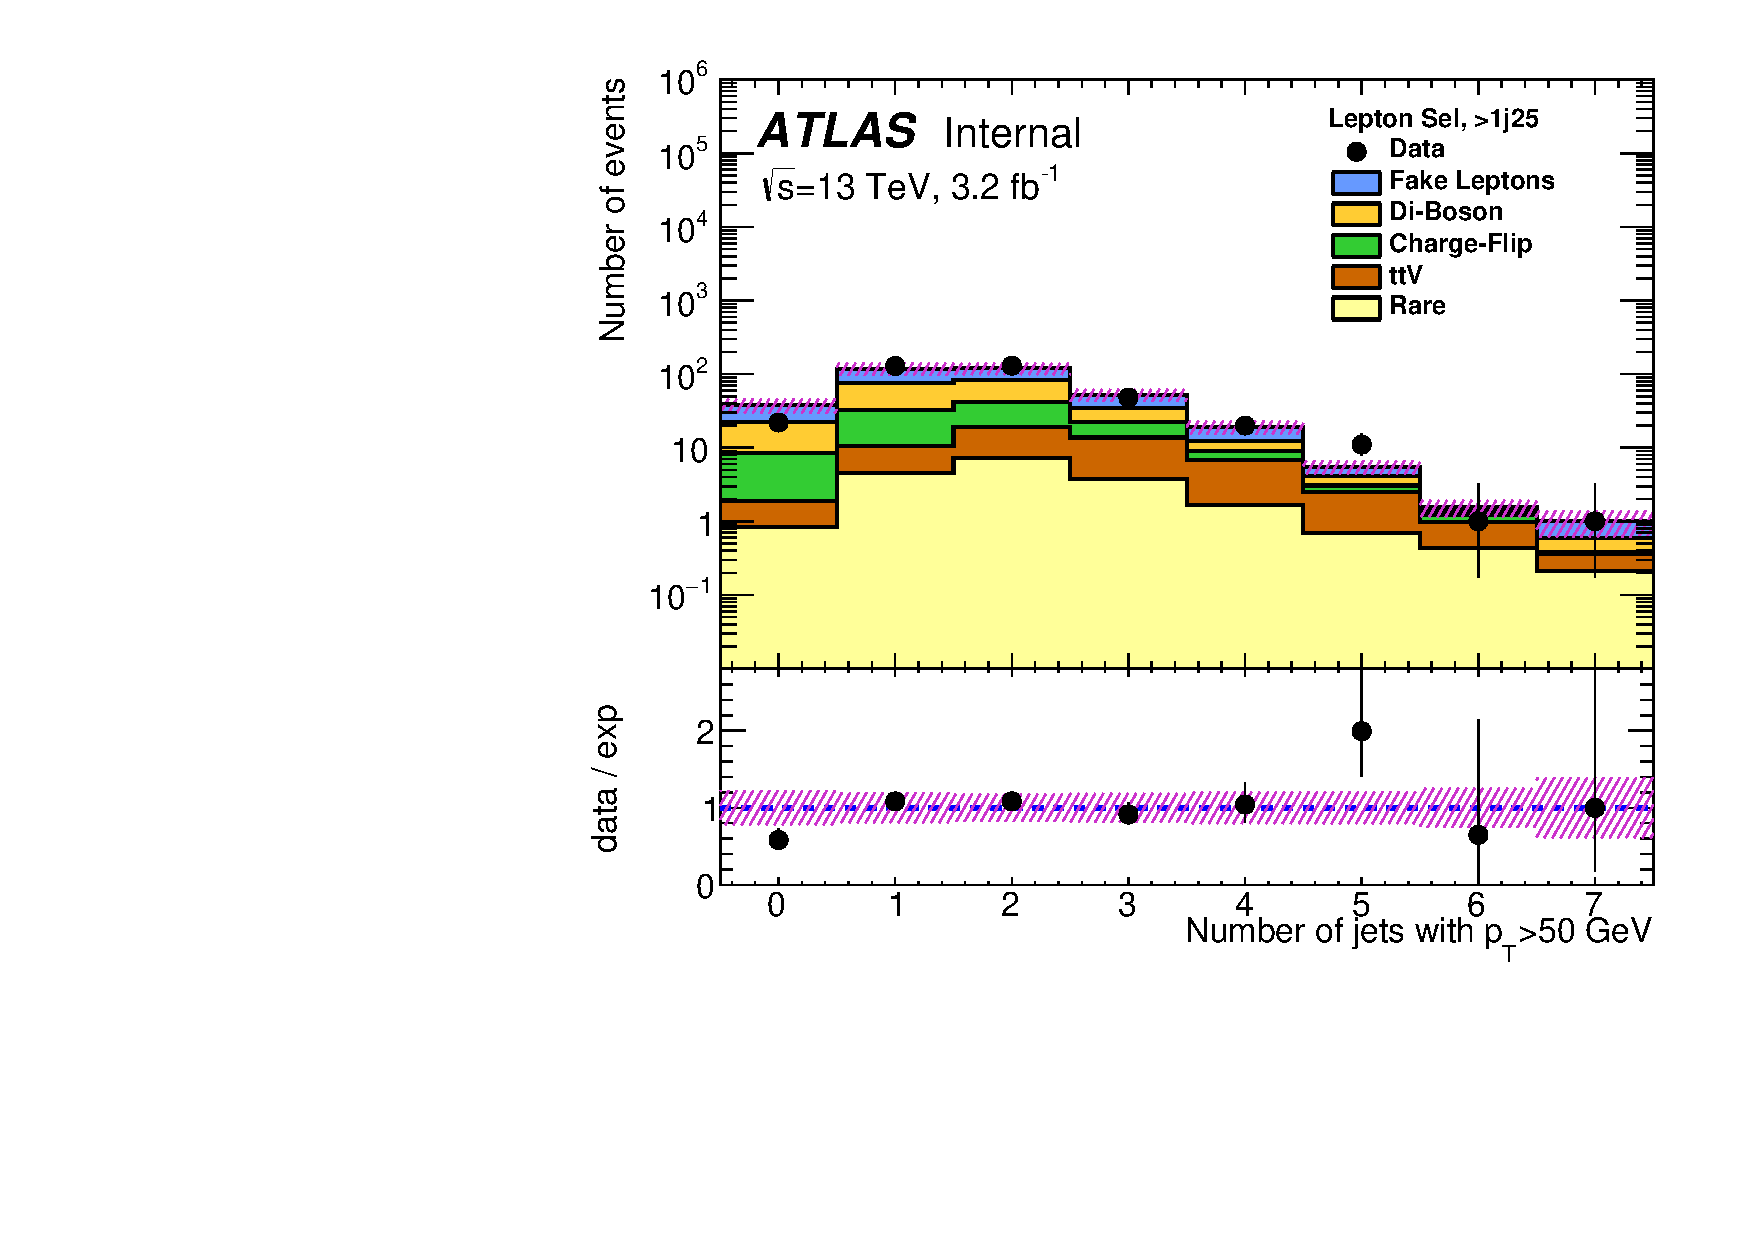
\includegraphics[width=0.45\textwidth]{BKG/validationPLots/NJETS50_LEP}
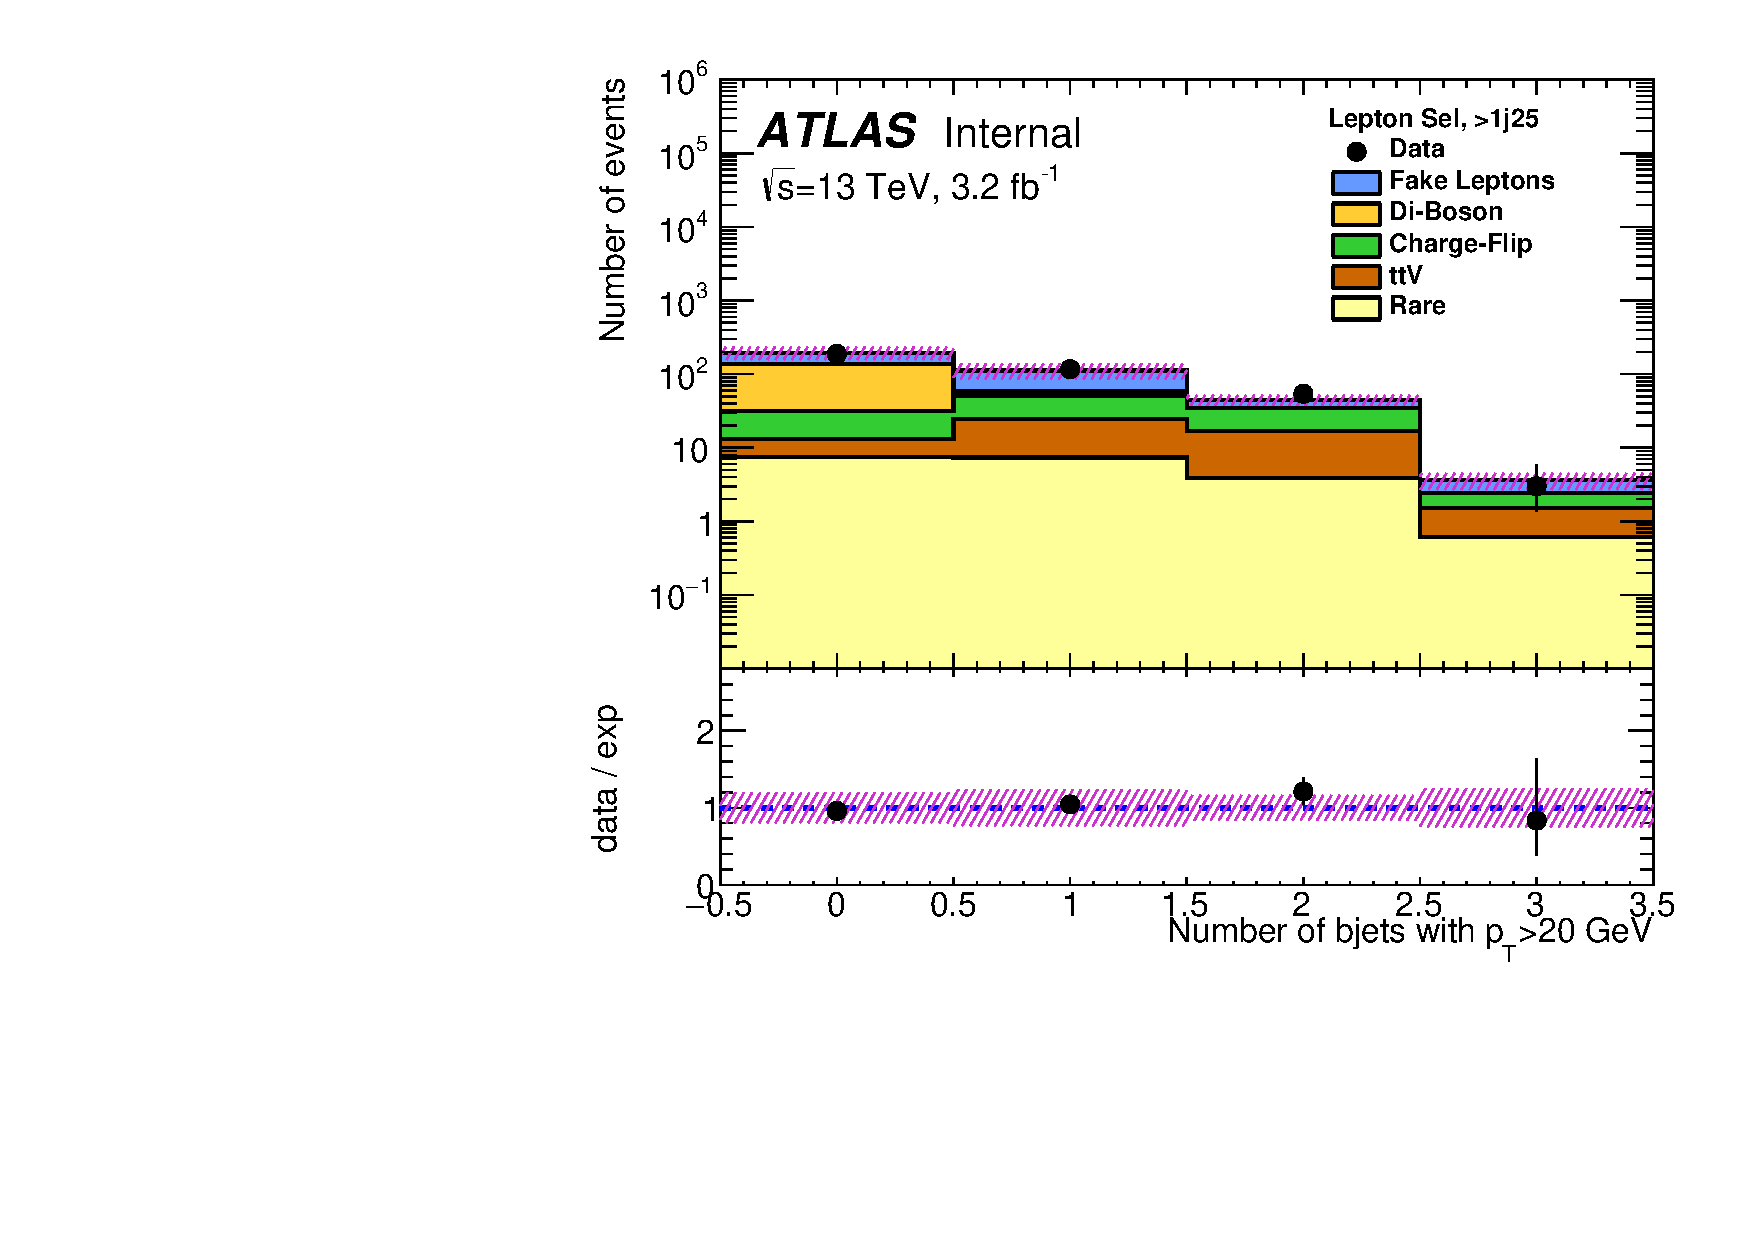
\includegraphics[width=0.45\textwidth]{BKG/validationPLots/NBJETS20_LEP}
}
\subfigure{
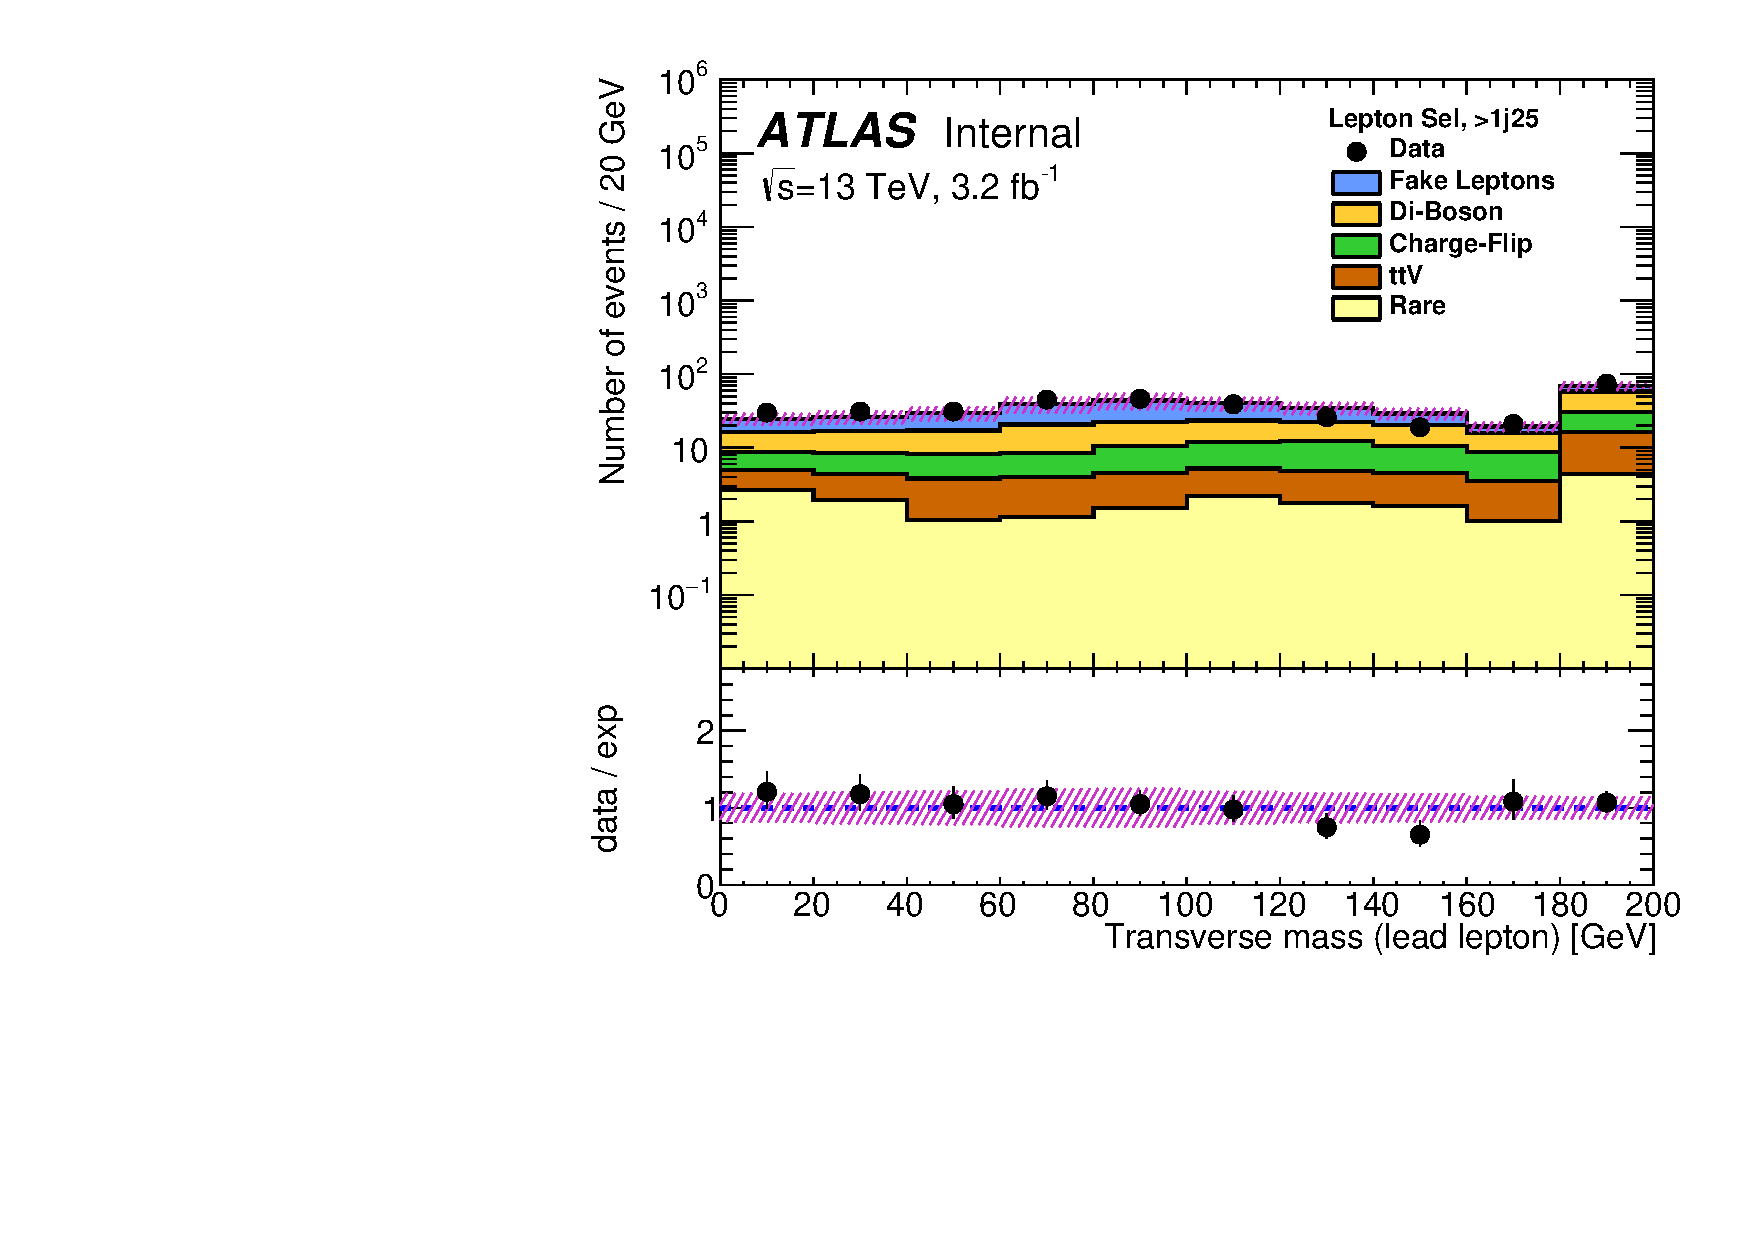
\includegraphics[width=0.45\textwidth]{BKG/validationPLots/MT_LEP_NOBJETCUT}
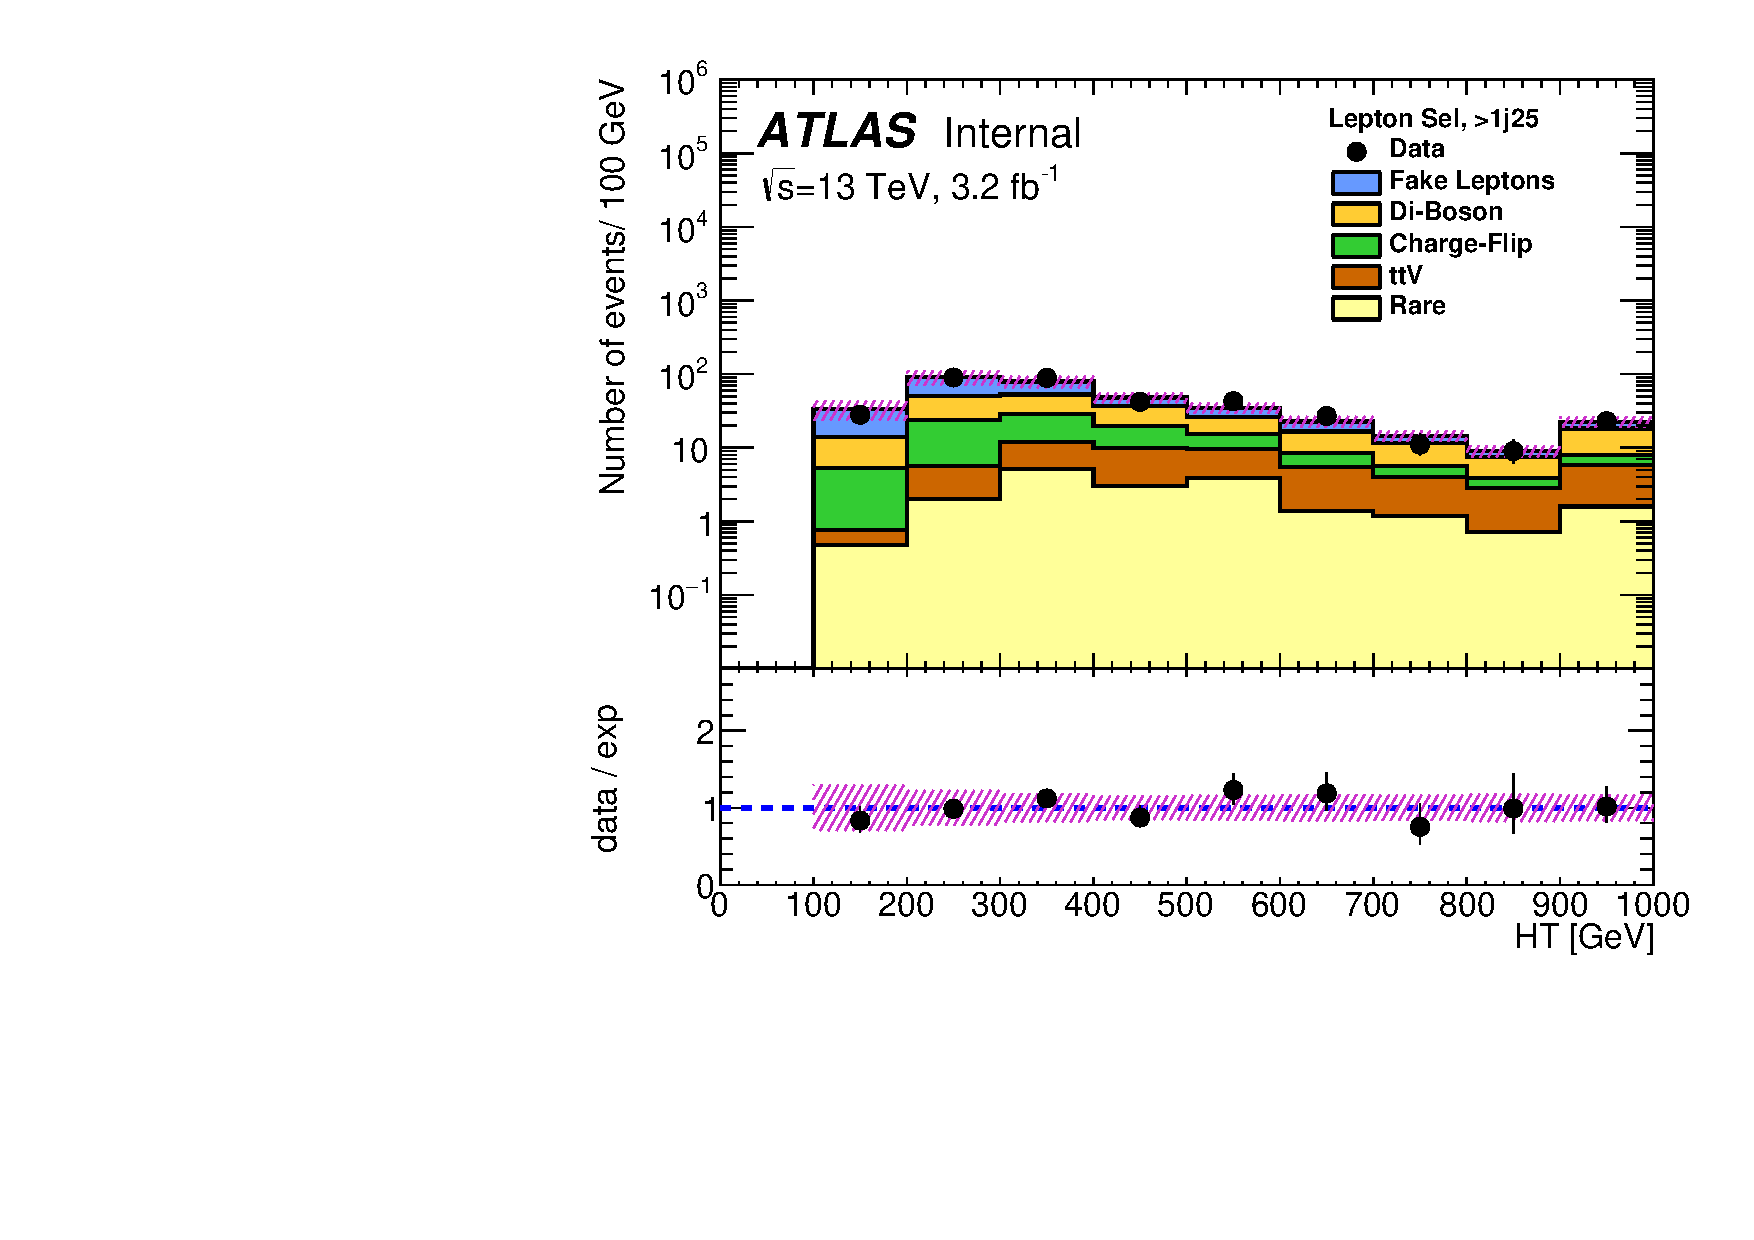
\includegraphics[width=0.45\textwidth]{BKG/validationPLots/HT_LEP_NOBJETCUT}
}
\subfigure{
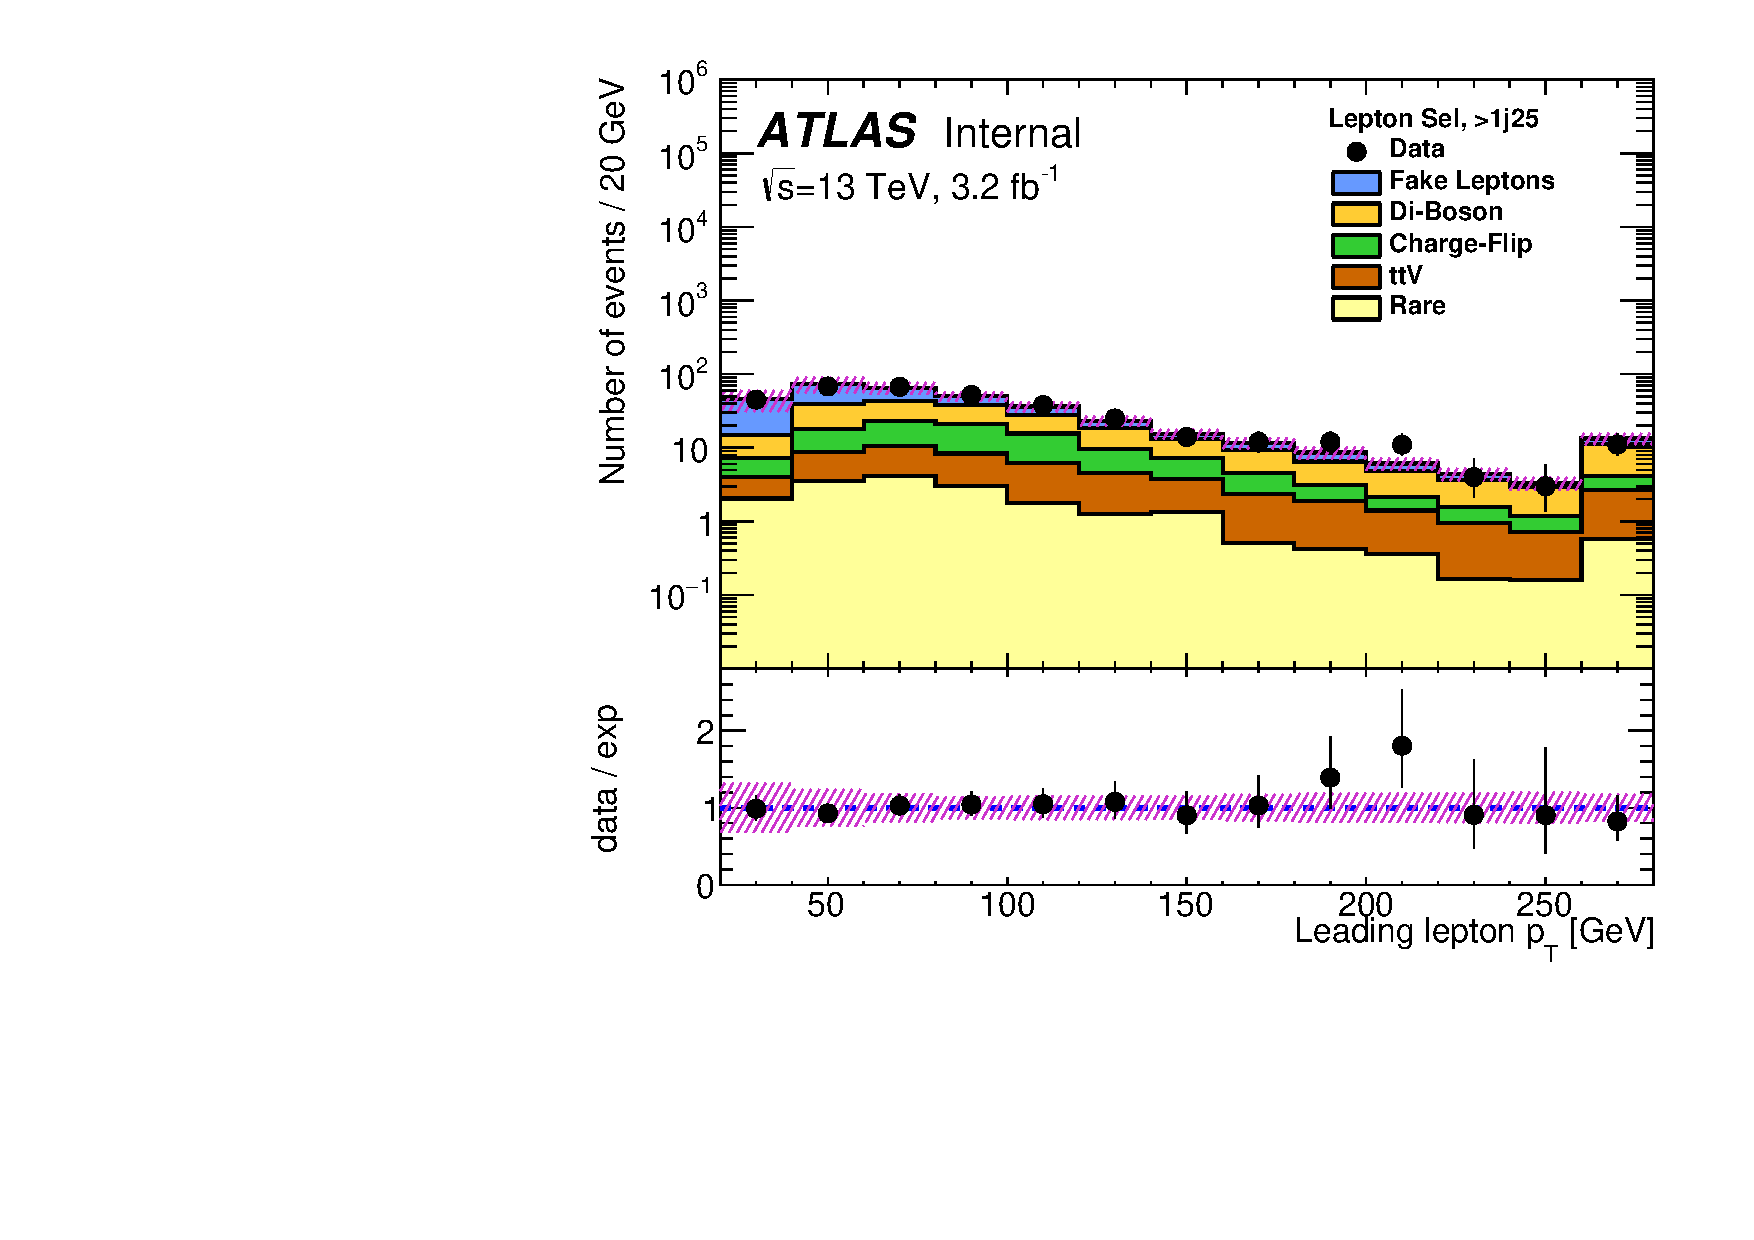
\includegraphics[width=0.45\textwidth]{BKG/validationPLots/PTLEP_LEAD_NOBJETCUT}
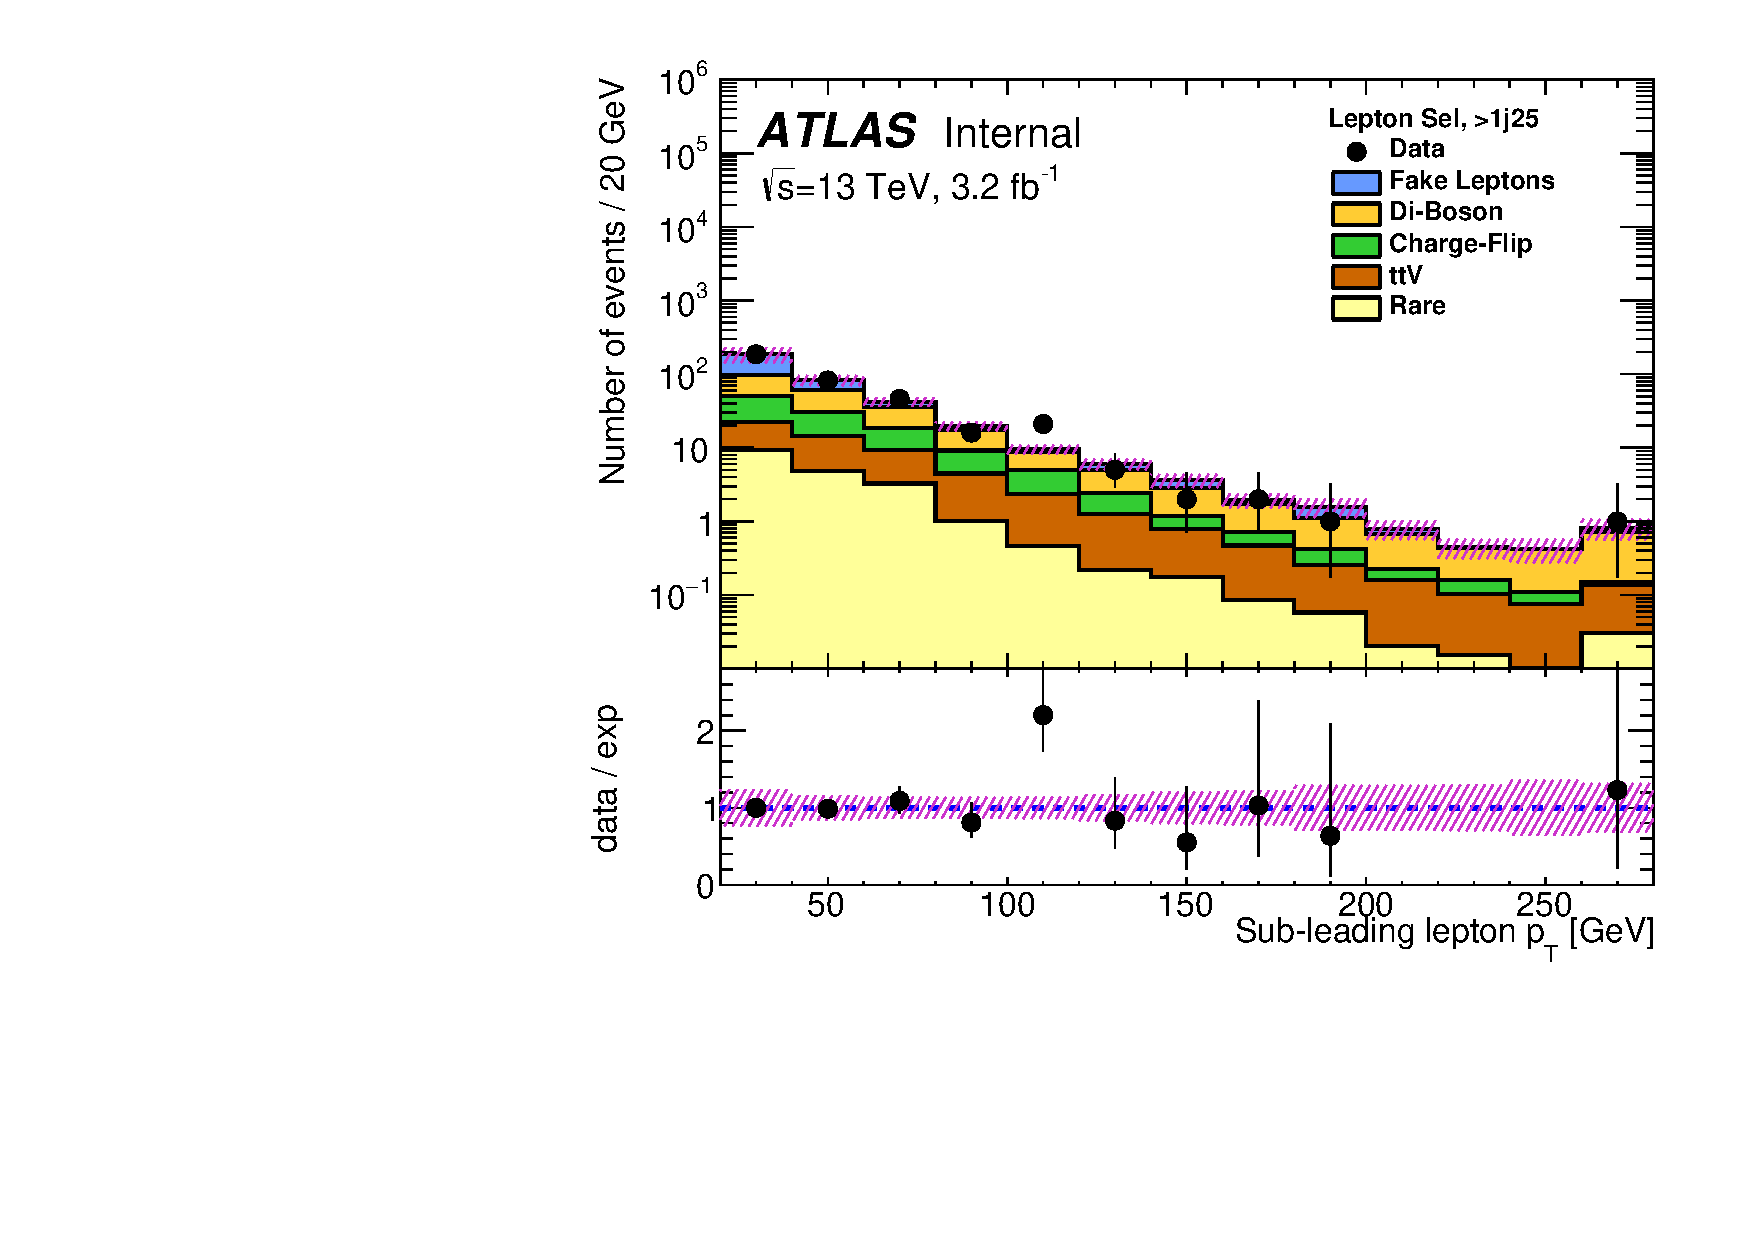
\includegraphics[width=0.45\textwidth]{BKG/validationPLots/PTLEP_SUBLEAD_NOBJETCUT}
}
\caption{$ee+e\mu+\mumu$ channel, \met $>$ 60\GeV and $N_{jets}^{25}$~$\ge$2: Distributions of  jet multiplicity (\pt~$>$~50~GeV) (top-left), $b$-jet multiplicity (\pt~$>$~20~GeV) (top-right), \mt (middle-left), $H_T$ (middle-right), leading lepton \pt (bottom-left) and subleading lepton \pt (bottom-right) after lepton selections.}
\label{Fig:VP_allCh_bIncl_Njets_and_other}
\end{figure} 

\FloatBarrier


%%%%% ee channel, >= 1 b-jet
\begin{figure}[h!]
\centering
\subfigure{
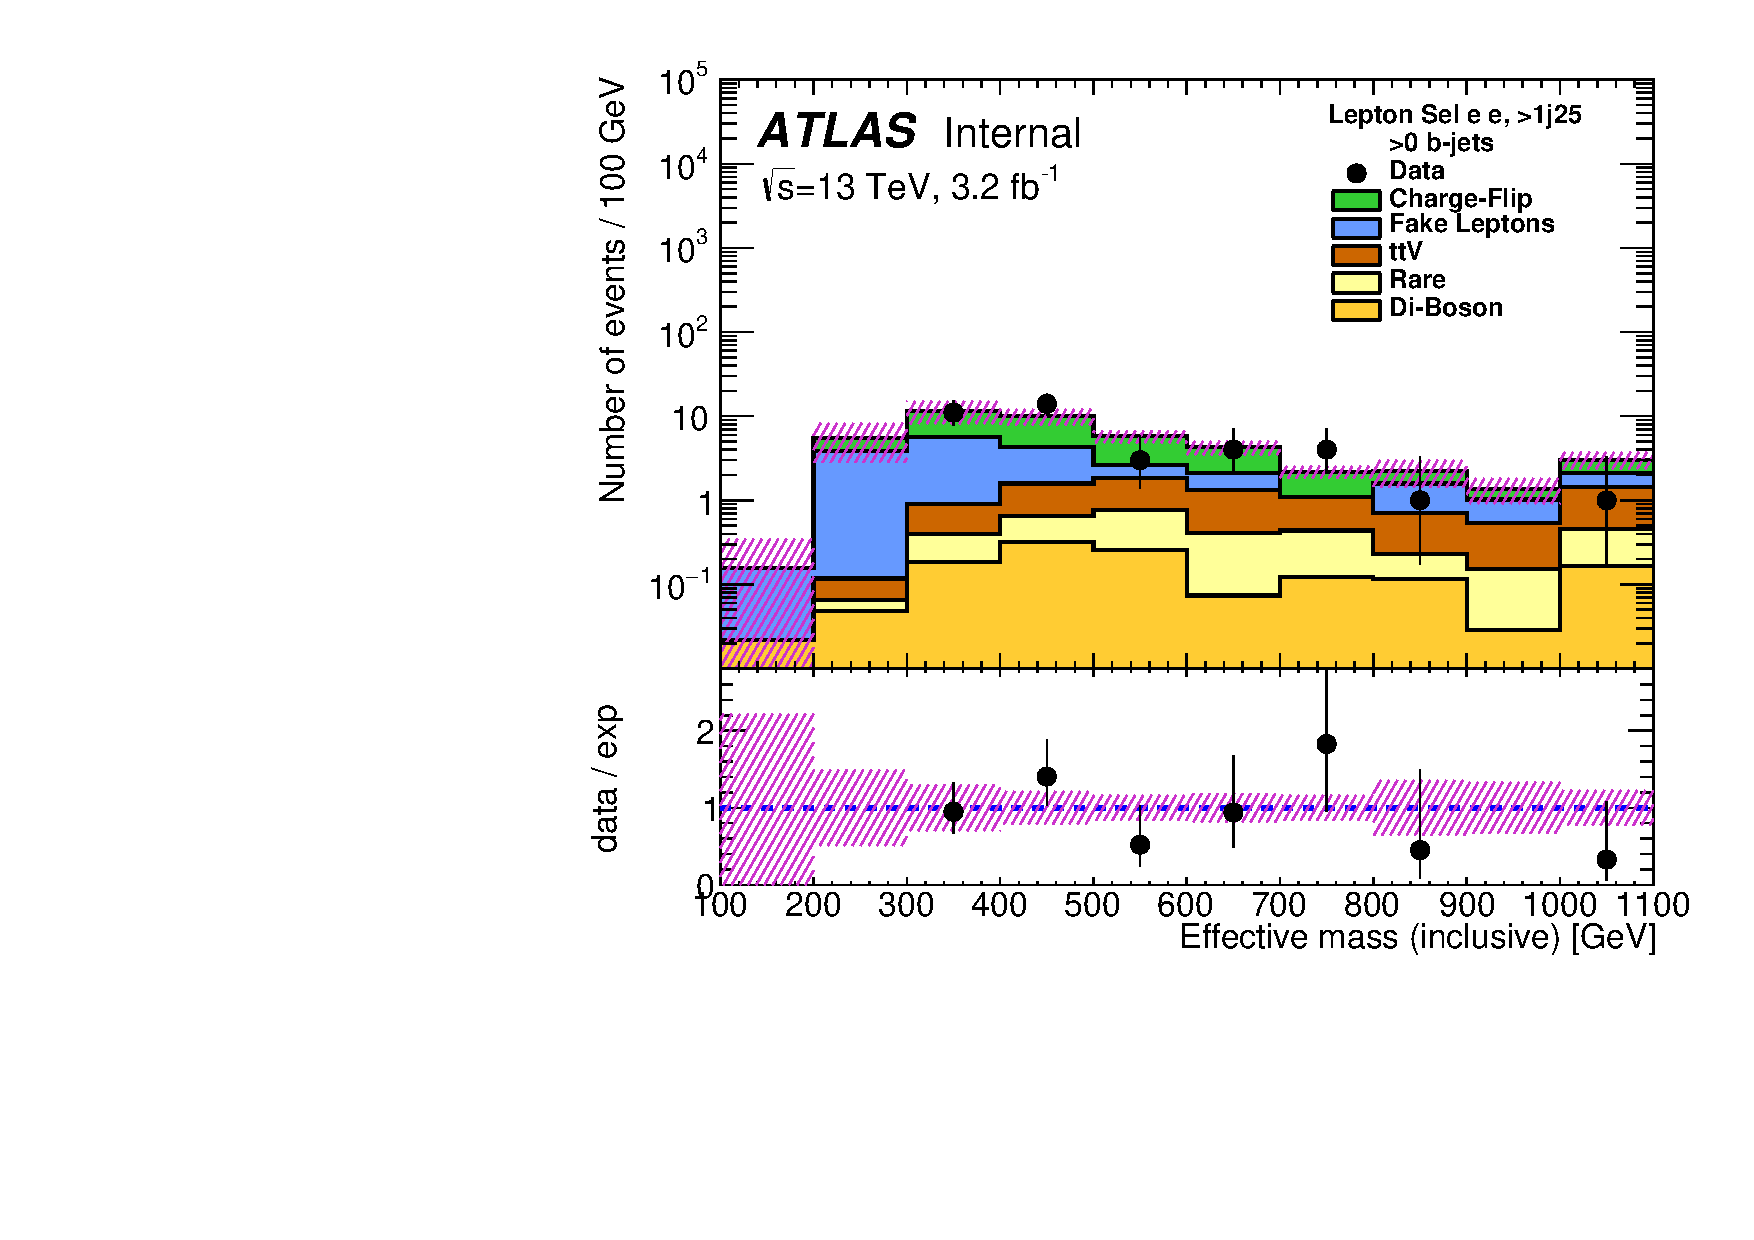
\includegraphics[width=0.5\textwidth]{BKG/validationPLots/MEFF_EE_LEP}
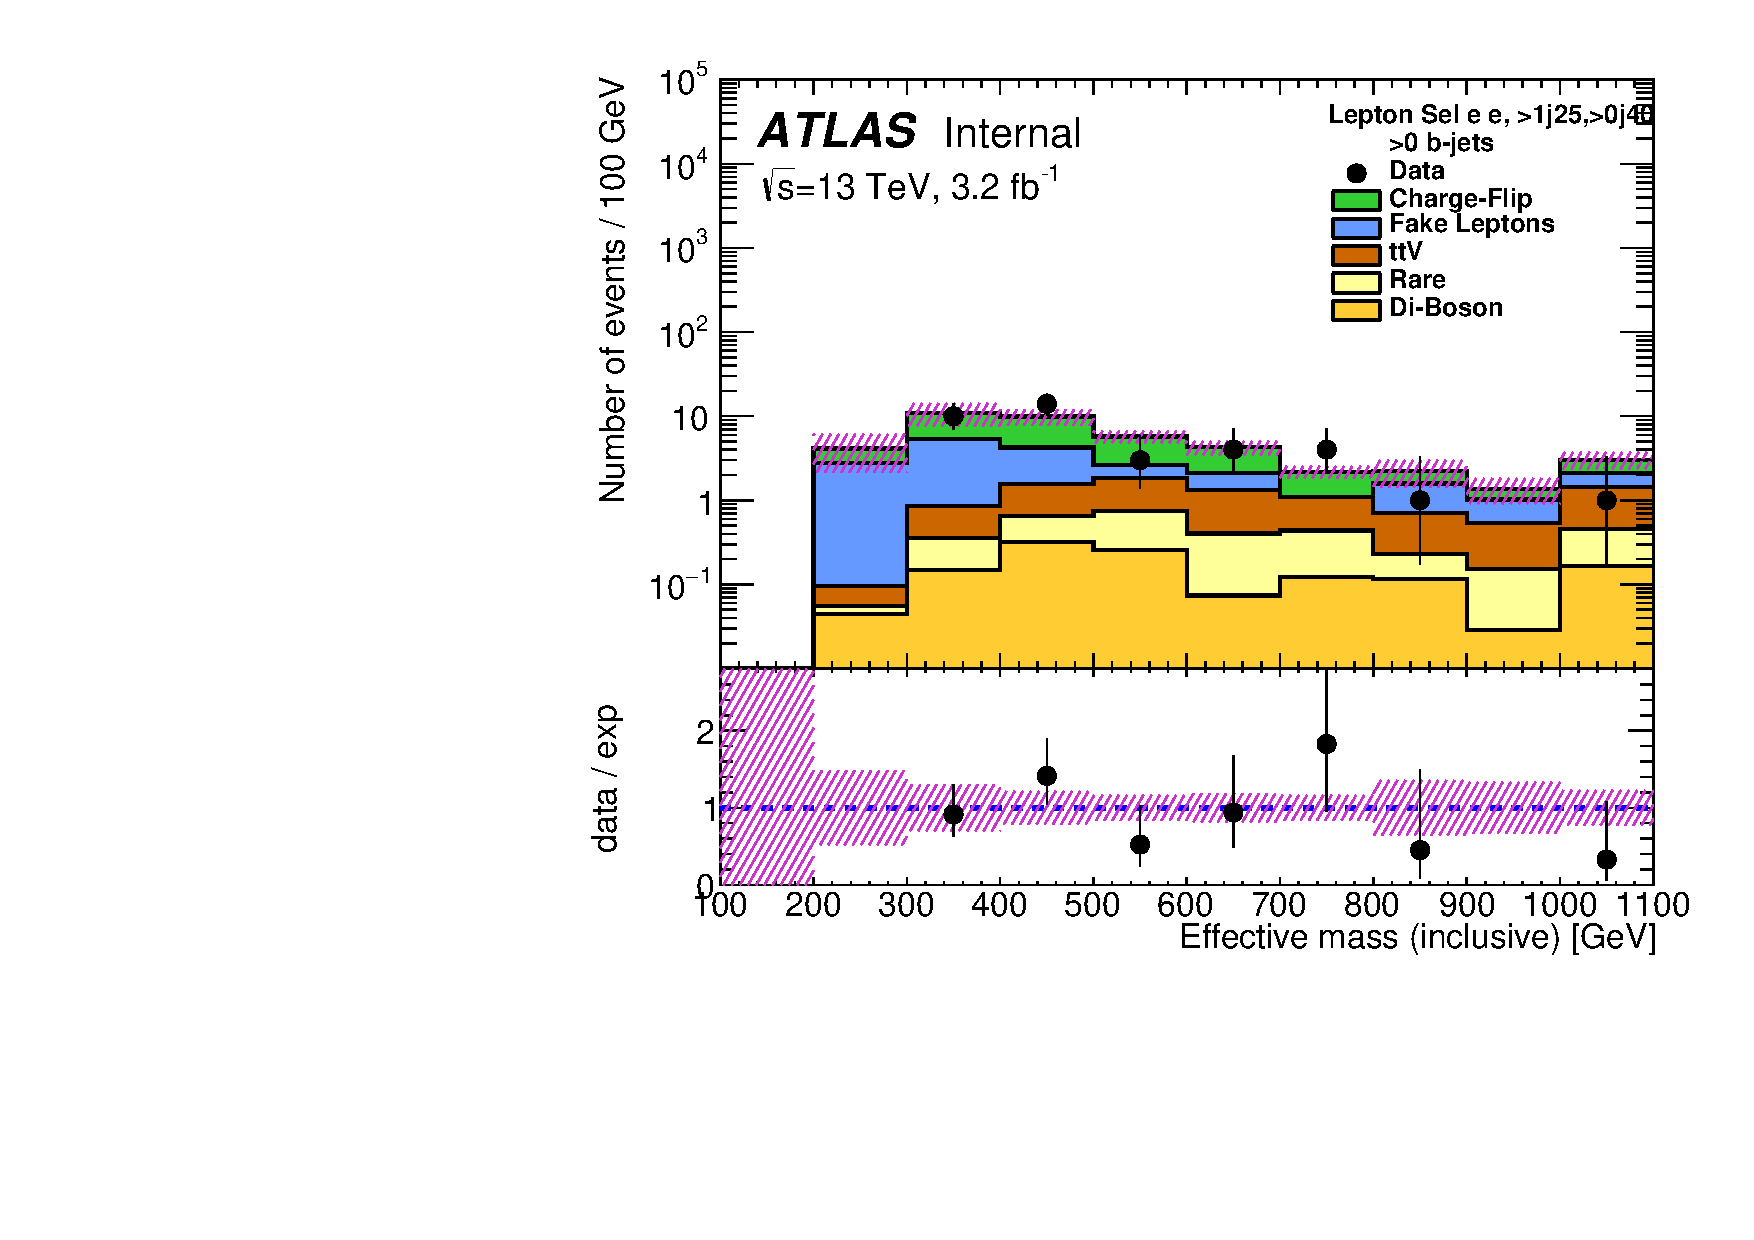
\includegraphics[width=0.5\textwidth]{BKG/validationPLots/MEFF_EE_L1JET}
}
\subfigure{
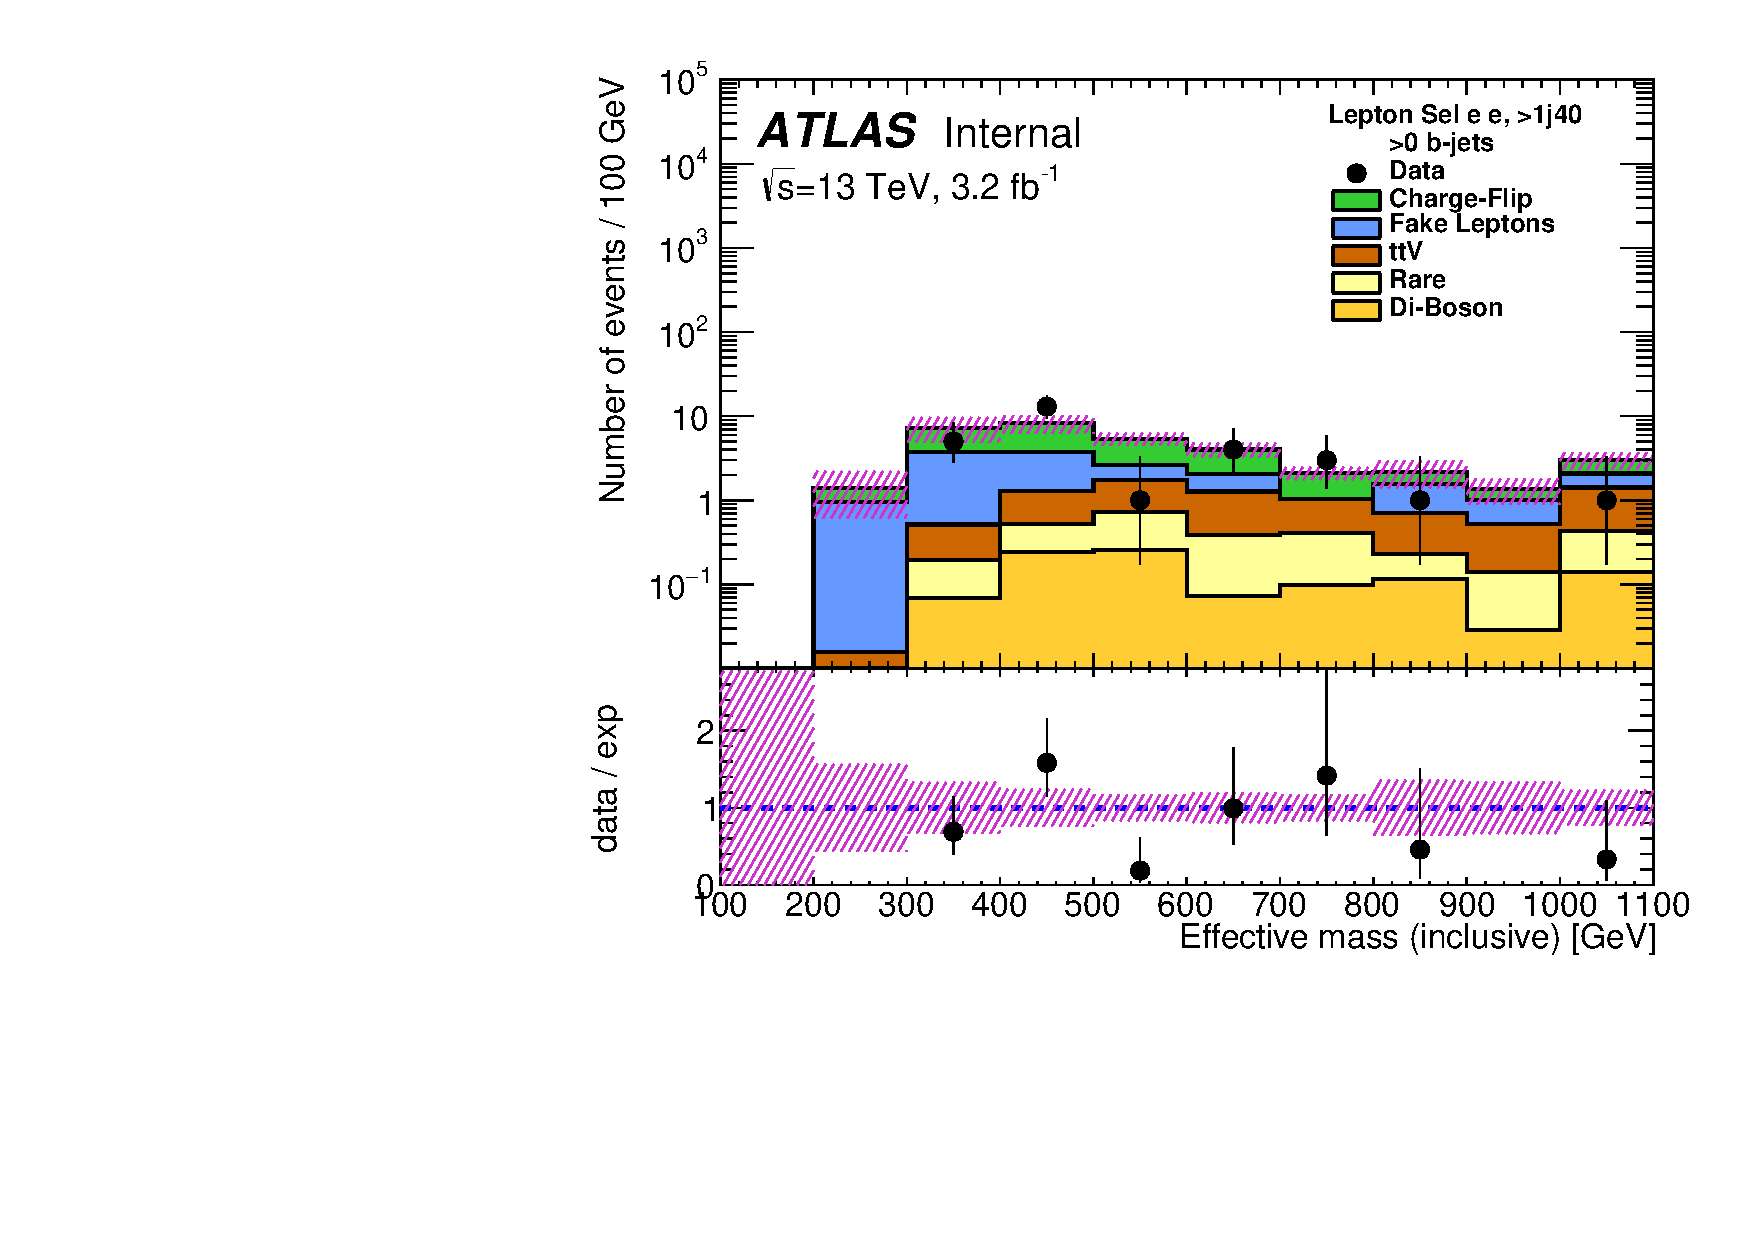
\includegraphics[width=0.5\textwidth]{BKG/validationPLots/MEFF_EE_L2JET}
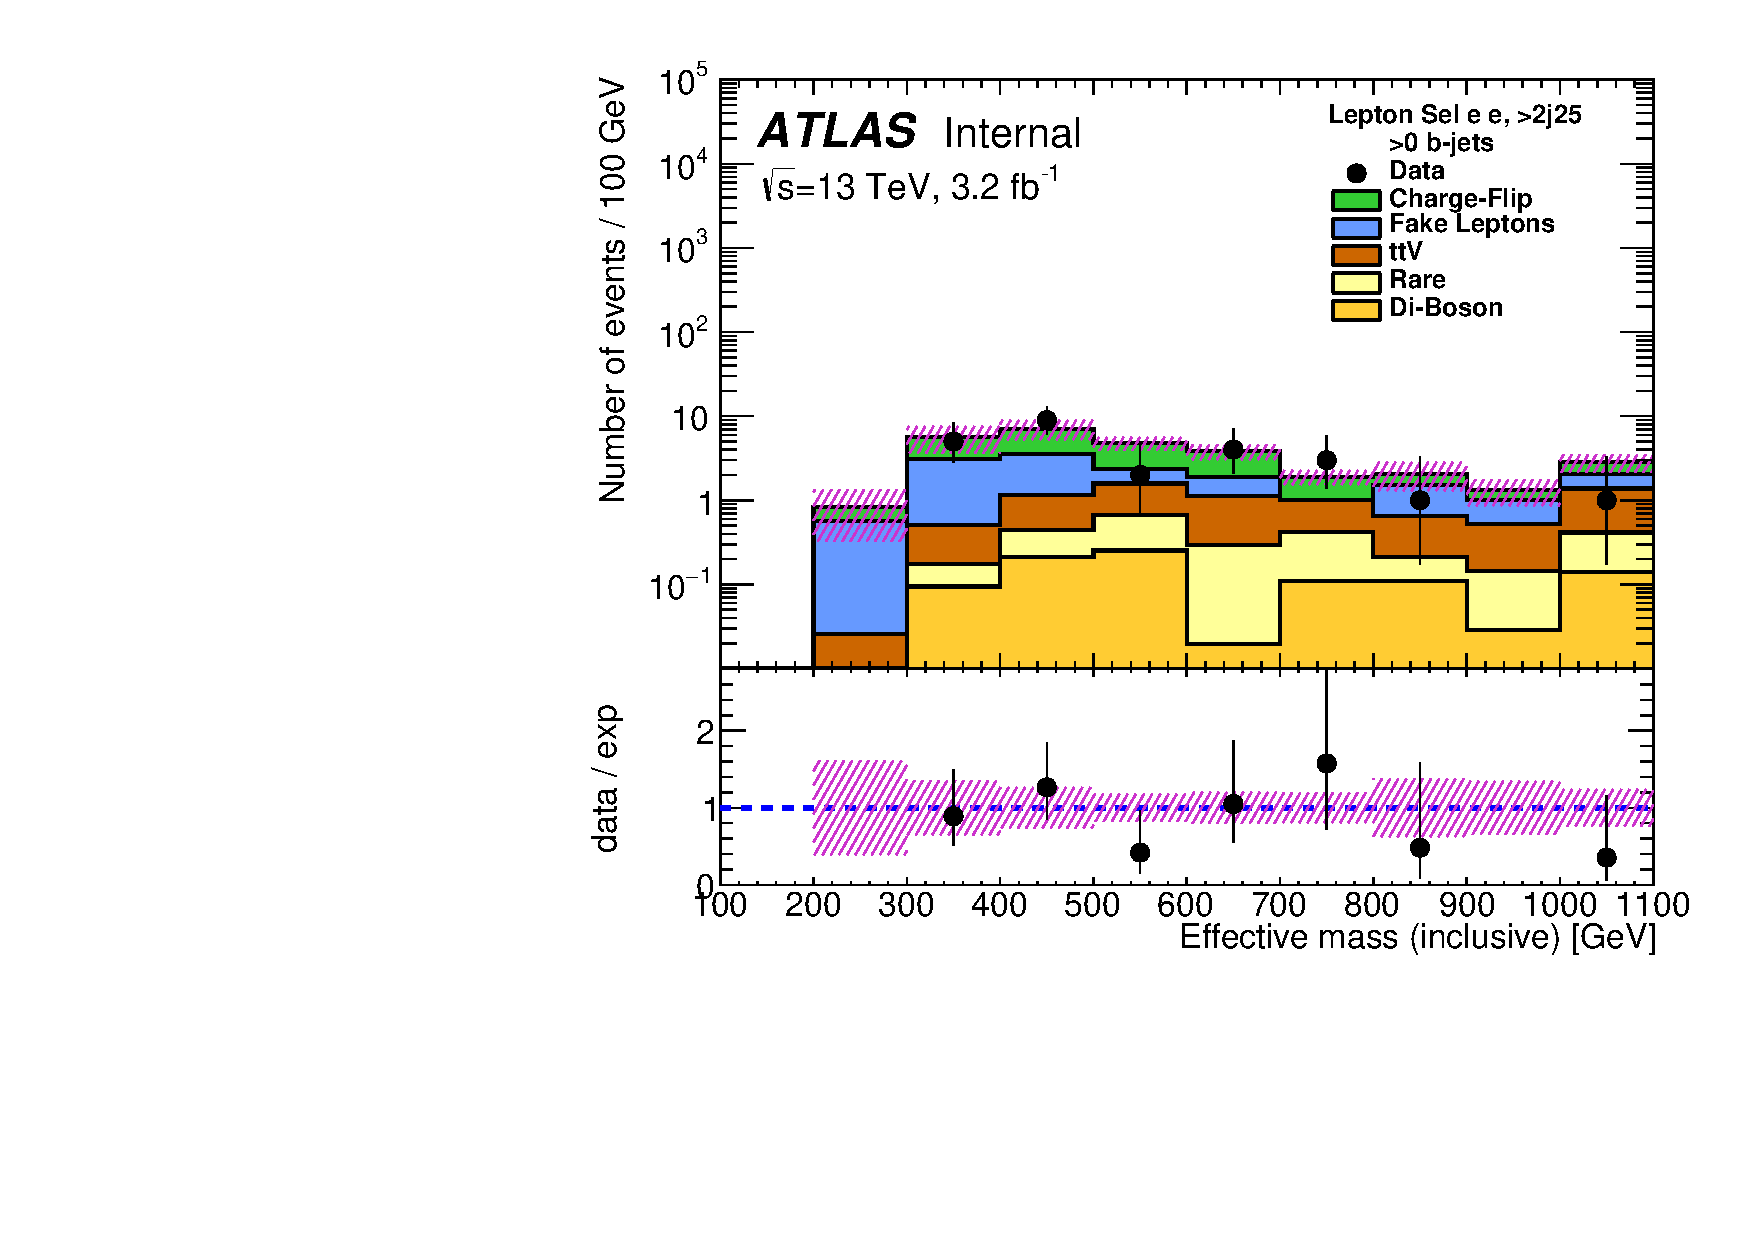
\includegraphics[width=0.5\textwidth]{BKG/validationPLots/MEFF_EE_L3JET}
}
\caption{$ee$ channel, \met $>$ 60\GeV and $N_{jets}^{25}$~$\ge$2: Effective mass distribution after lepton selections with at least one $b$-jet (\pt~$>$~20~GeV) and with at least 0, 1, 2 and 3 jets with \pt~$>$~40~GeV (from top-left to bottom-right).}
\label{Fig:VP_ee_1b_Meff}
\end{figure}
%%
\begin{figure}[h!]
\centering
\subfigure{
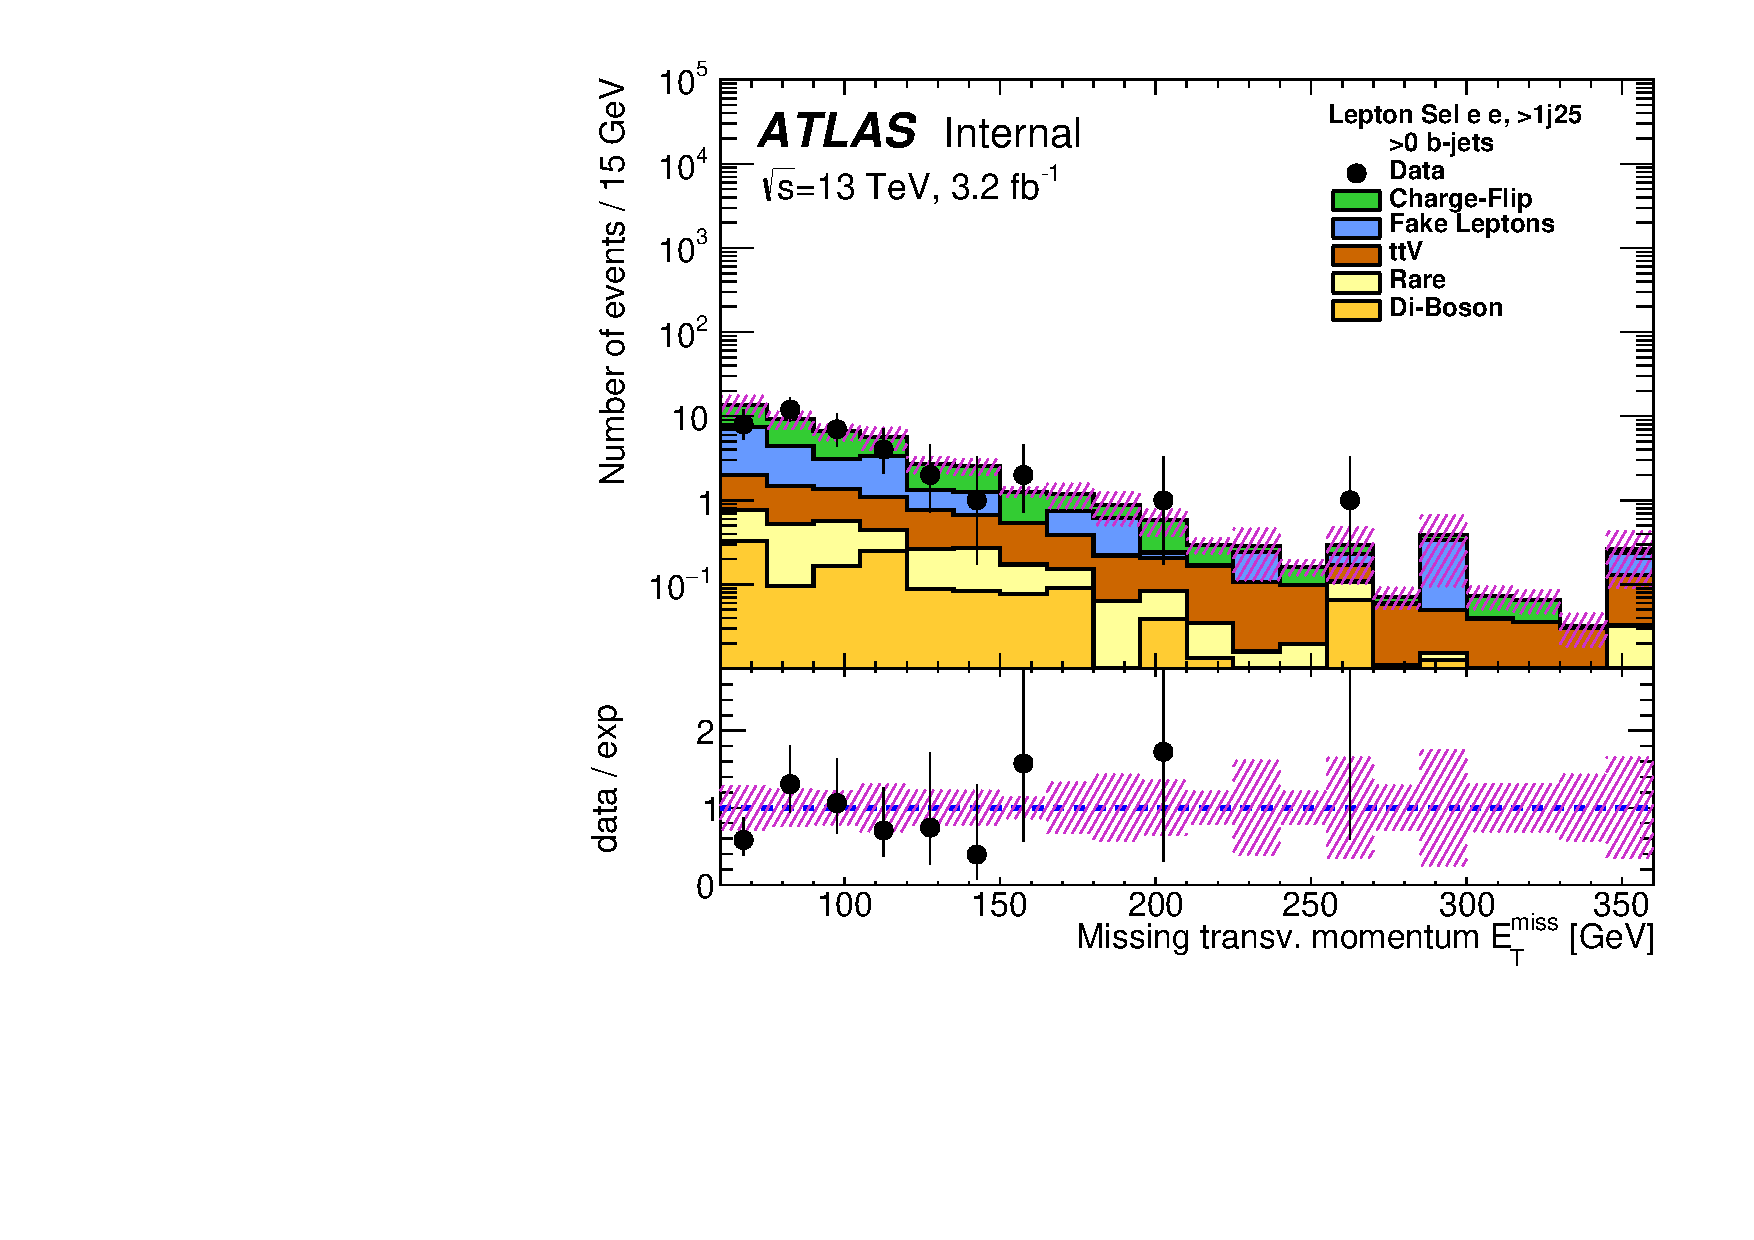
\includegraphics[width=0.5\textwidth]{BKG/validationPLots/MET_EE_LEP}
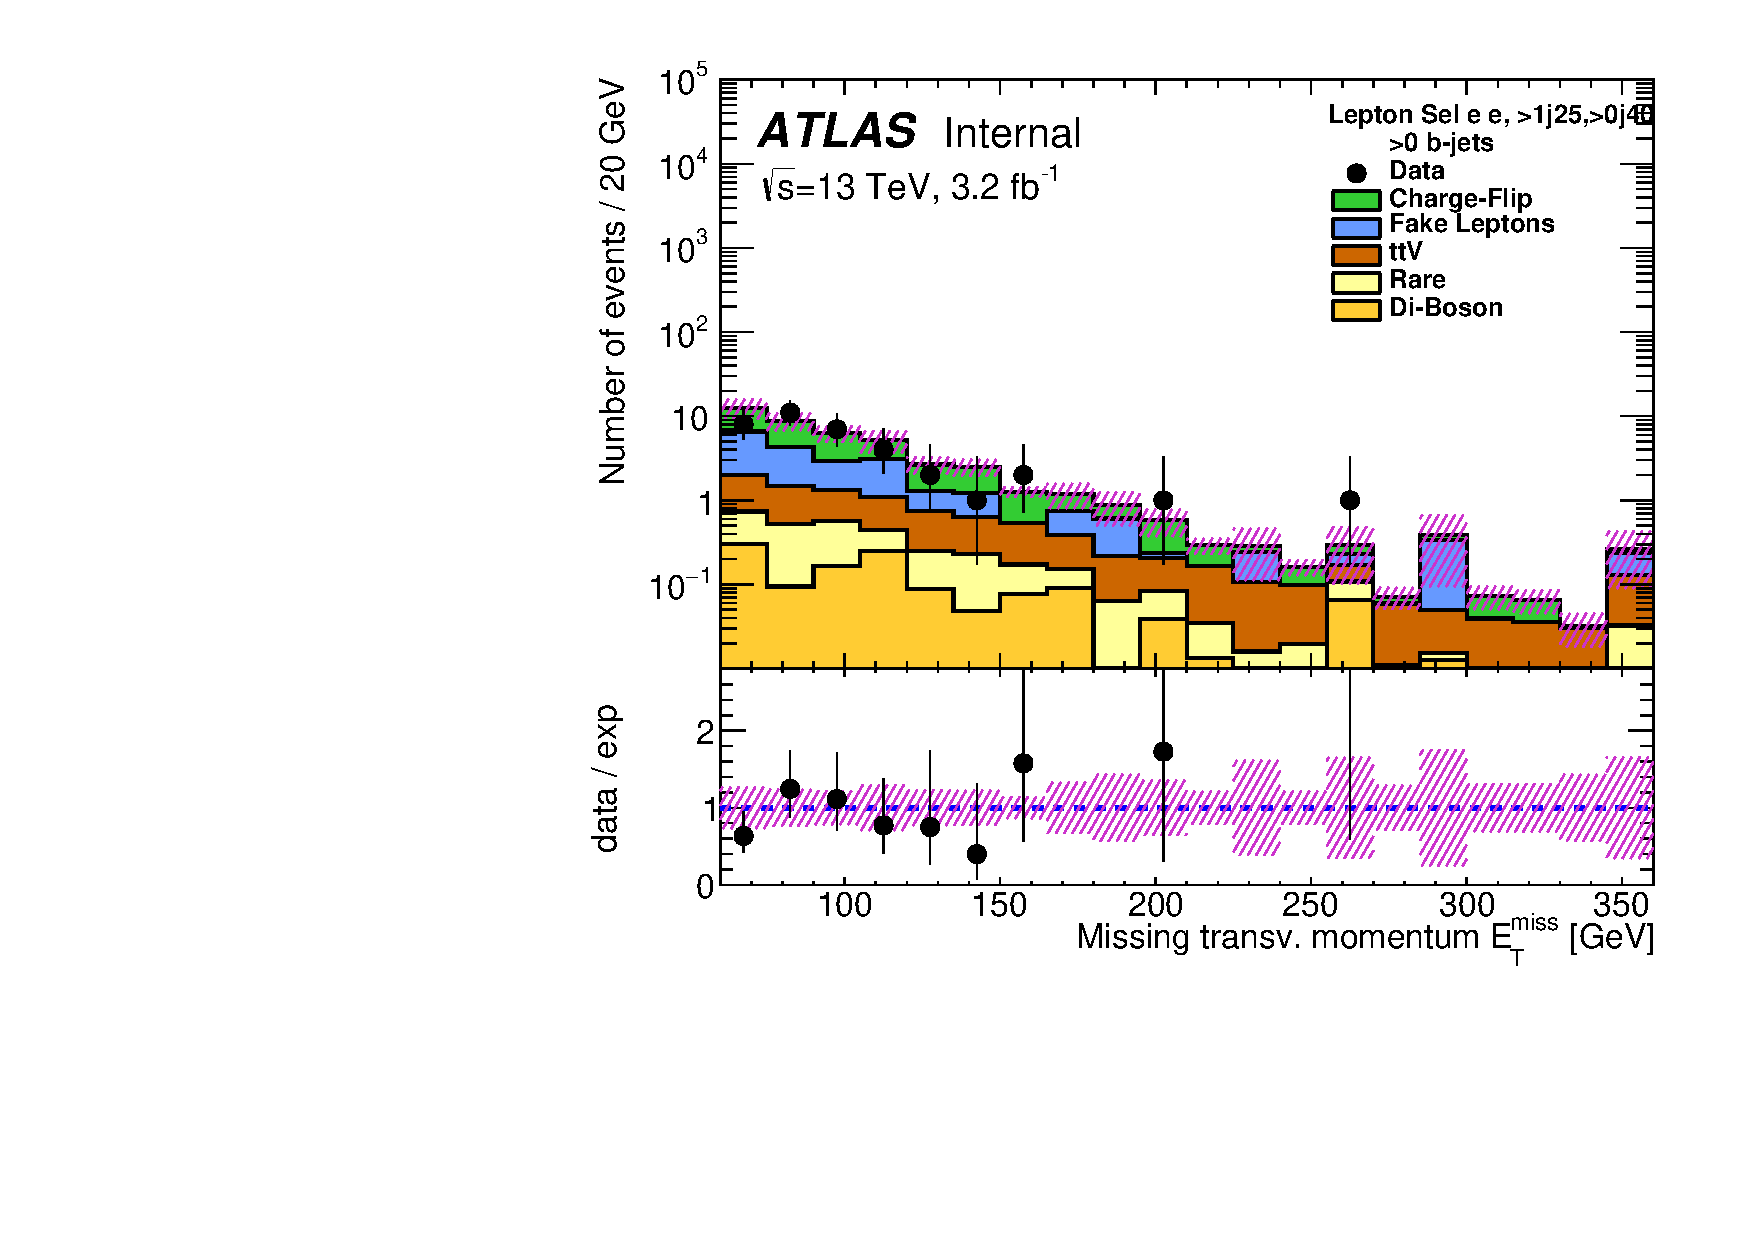
\includegraphics[width=0.5\textwidth]{BKG/validationPLots/MET_EE_L1JET}
}
\subfigure{
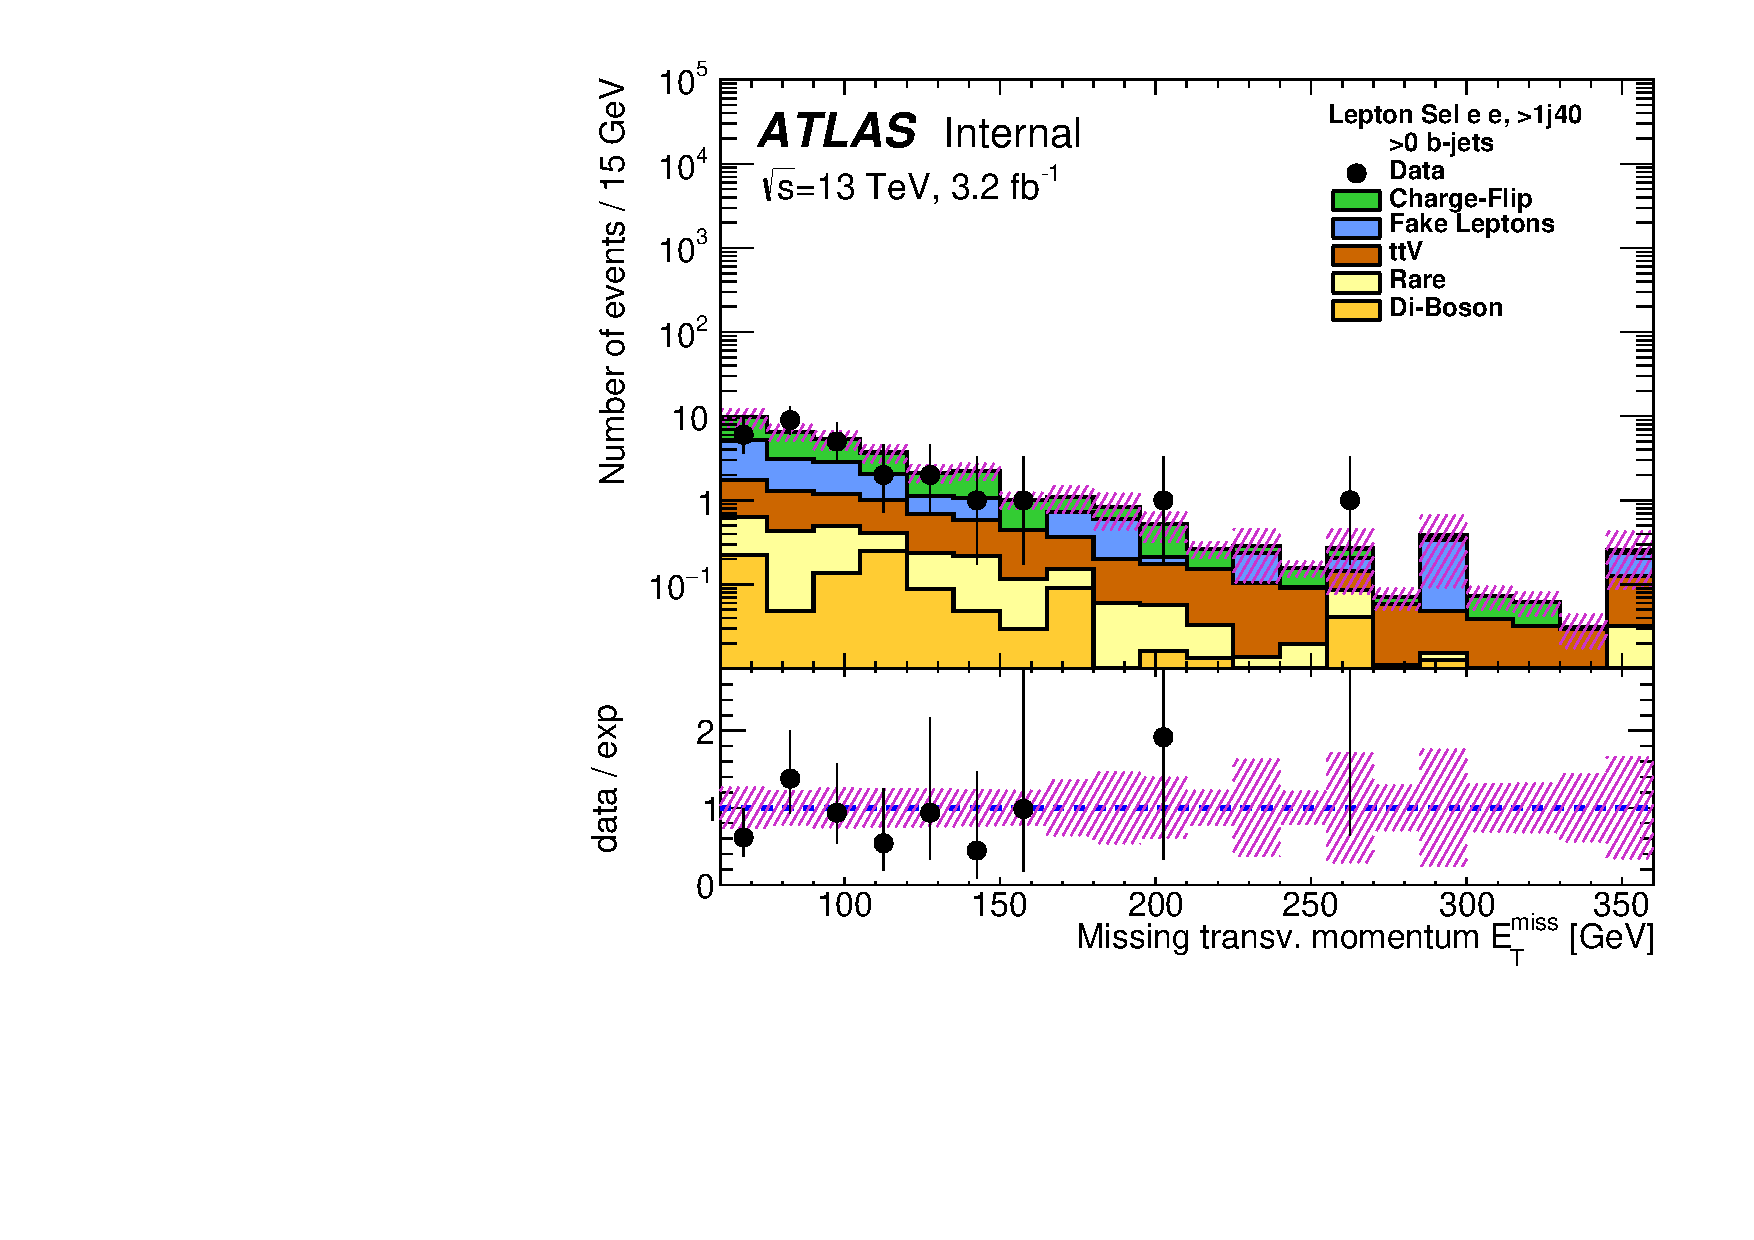
\includegraphics[width=0.5\textwidth]{BKG/validationPLots/MET_EE_L2JET}
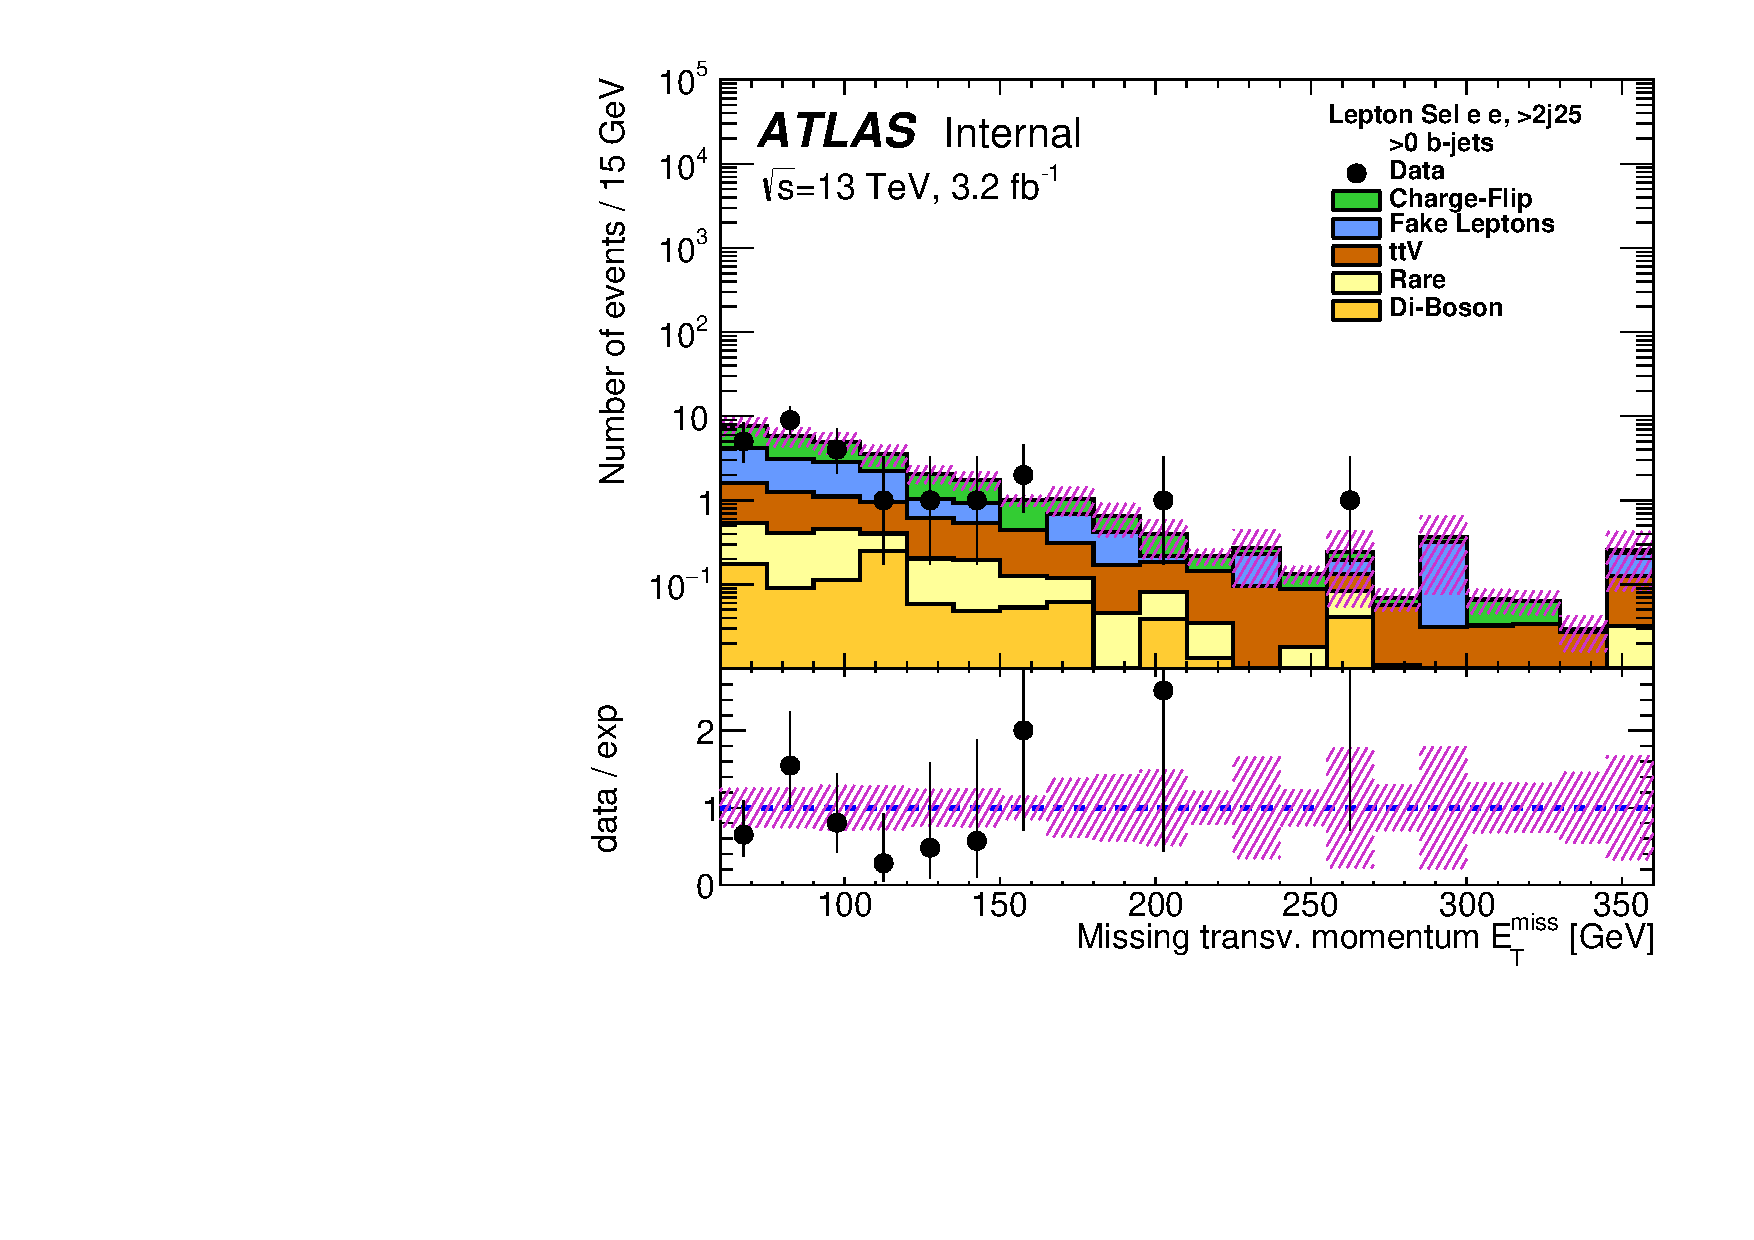
\includegraphics[width=0.5\textwidth]{BKG/validationPLots/MET_EE_L3JET}
}
\caption{$ee$ channel, \met $>$ 60\GeV and $N_{jets}^{25}$~$\ge$2: Missing transverse energy distribution after lepton selections with at least one $b$-jet (\pt~$>$~20~GeV) and with at least 0, 1, 2 and 3 jets with \pt~$>$~40~GeV (from top-left to bottom-right).}
\label{Fig:VP_ee_1b_Met}
\end{figure}
%%
\begin{figure}[h!]
\centering
\subfigure{
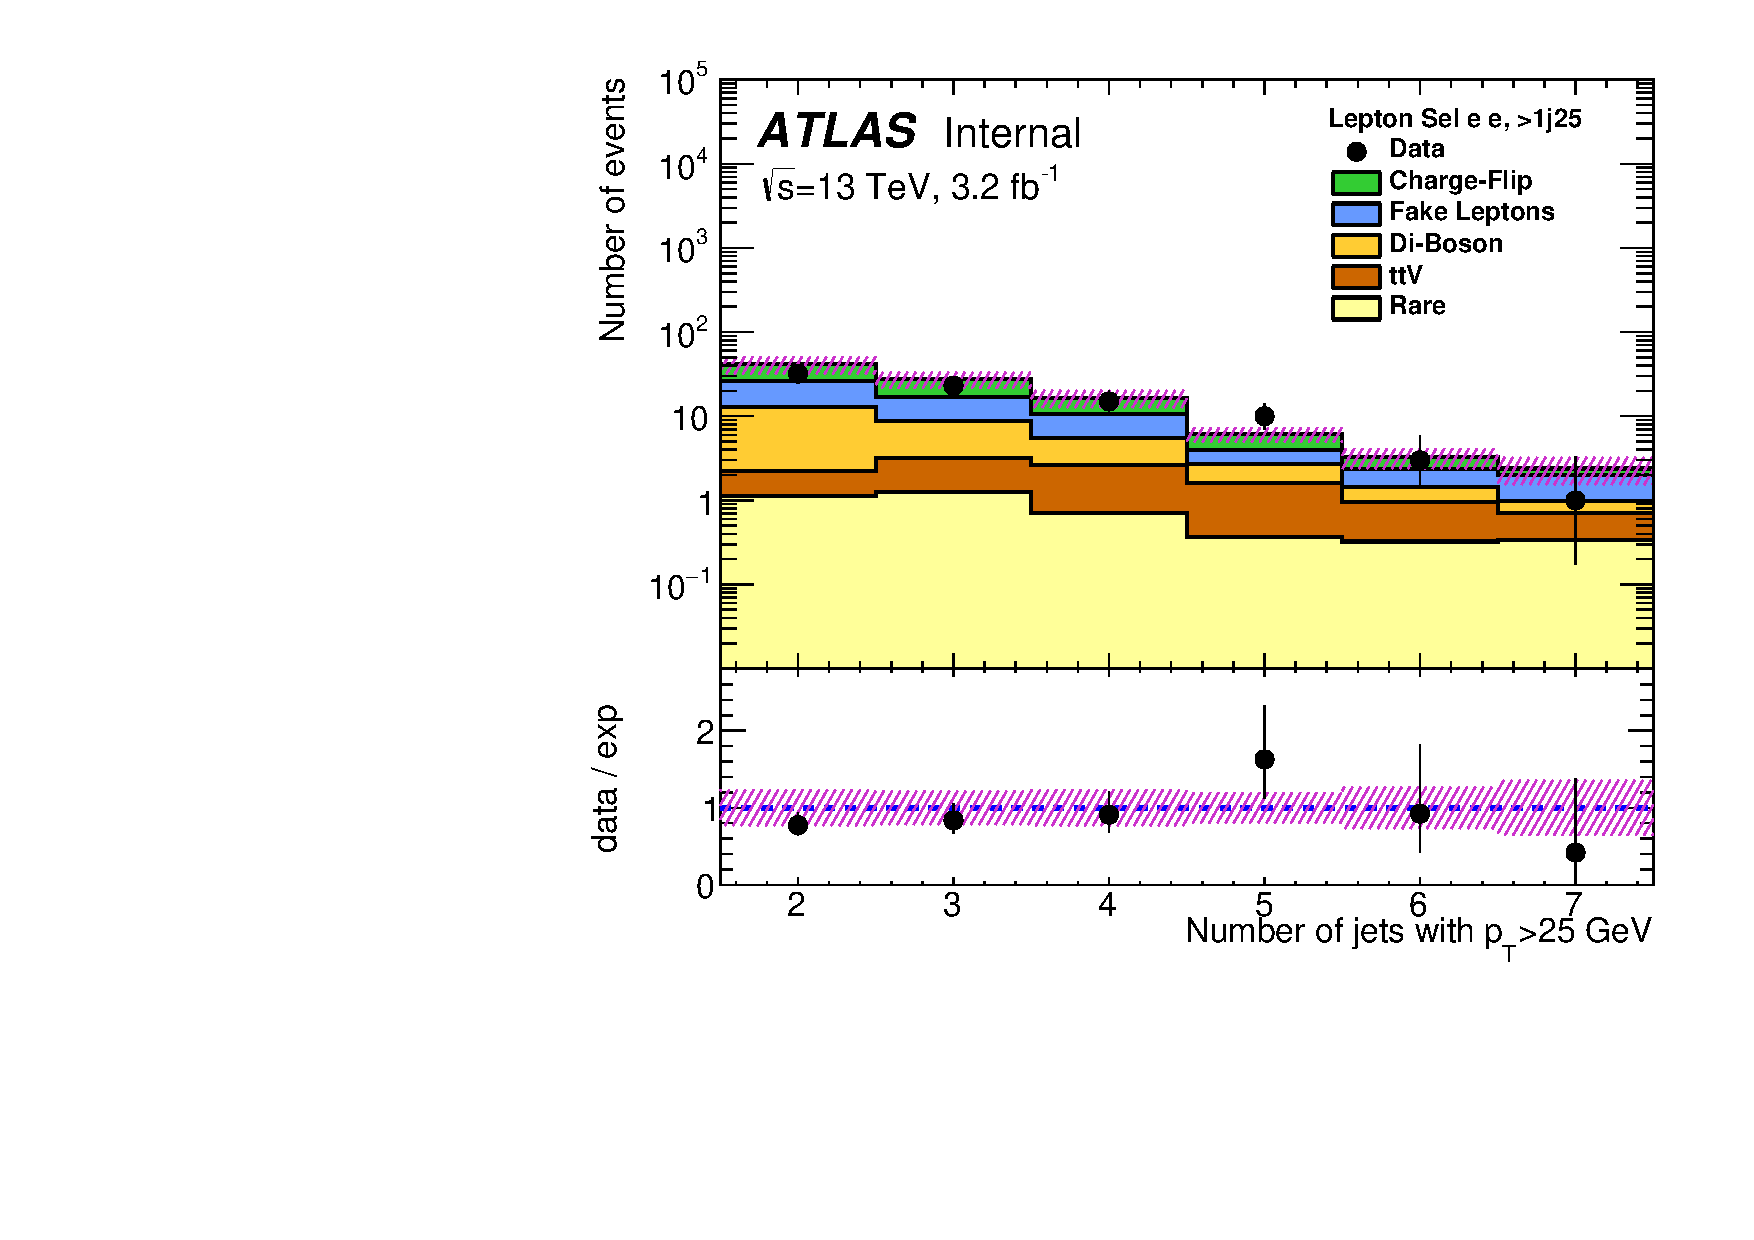
\includegraphics[width=0.45\textwidth]{BKG/validationPLots/NJETS40_EE_LEP}
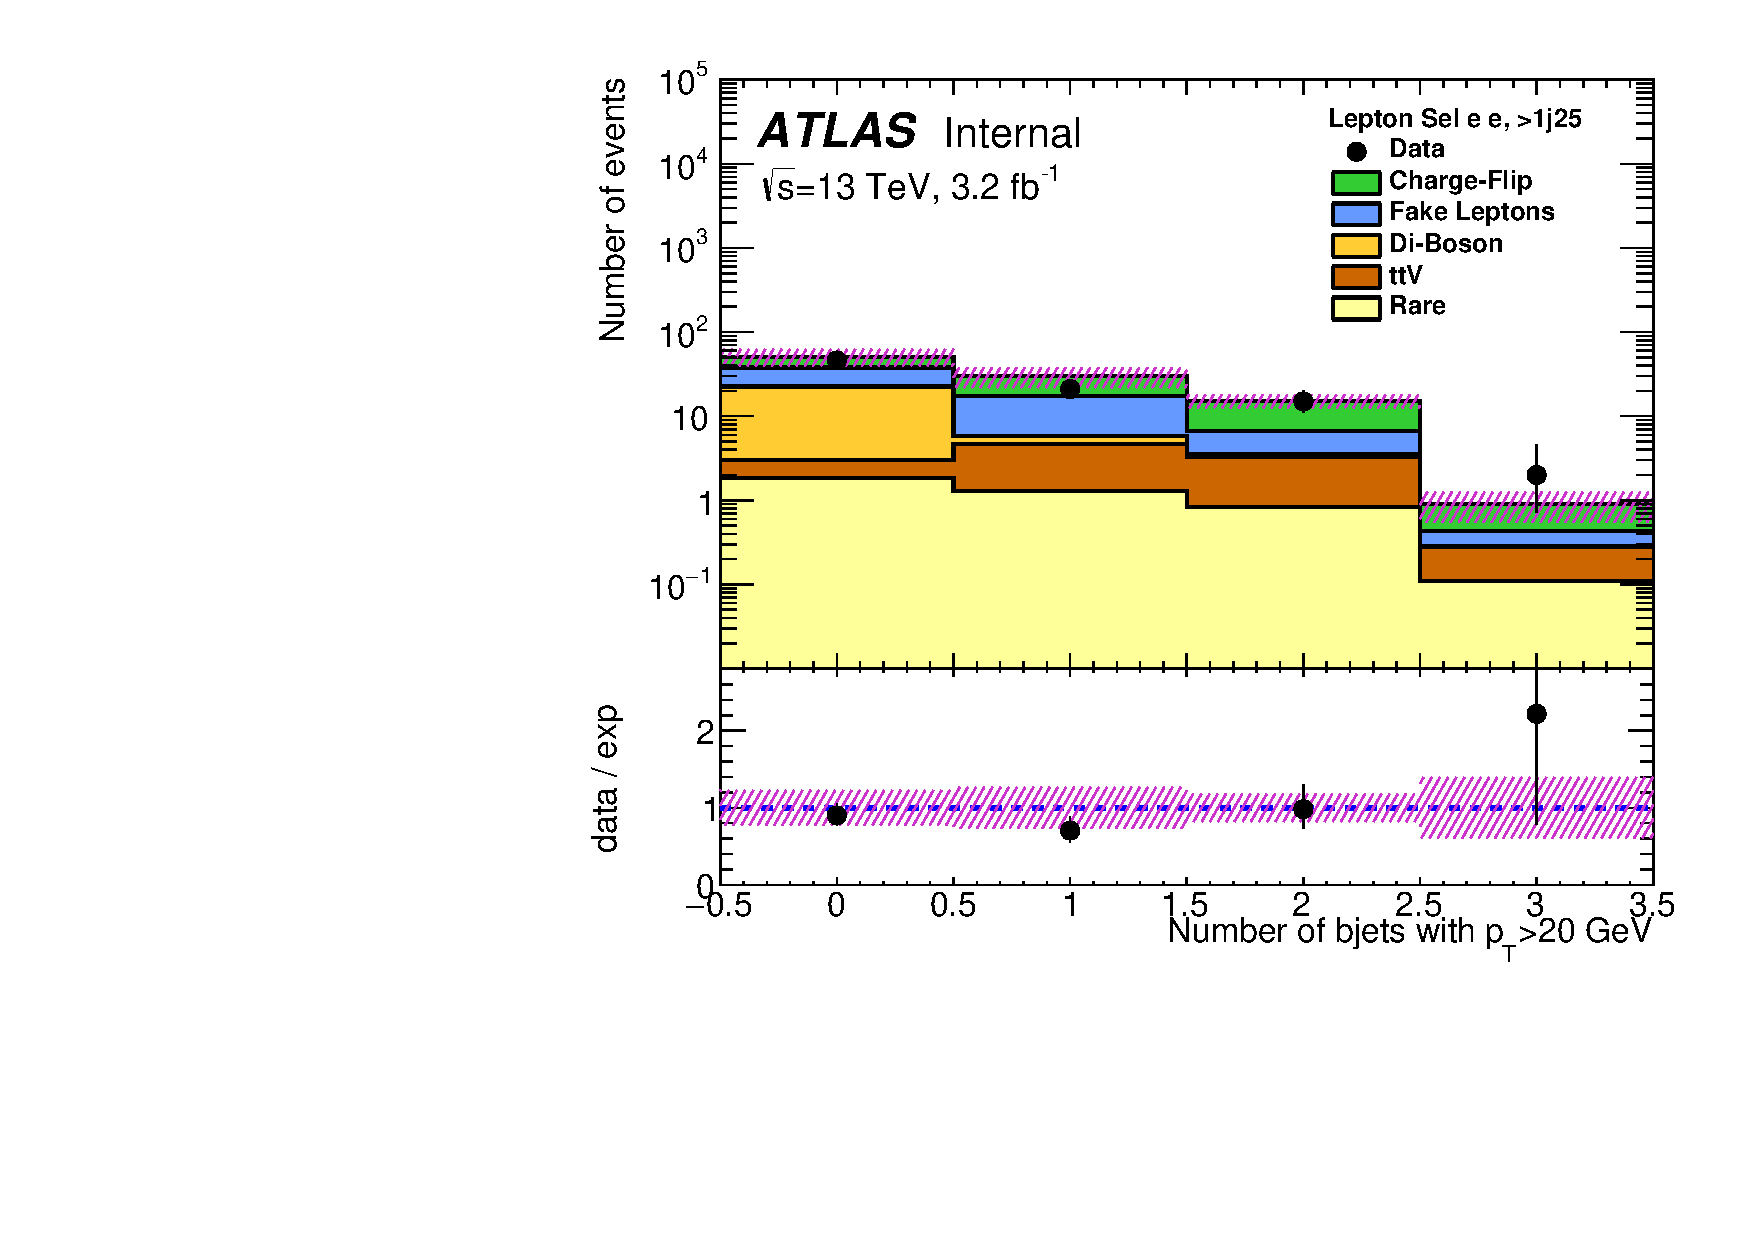
\includegraphics[width=0.45\textwidth]{BKG/validationPLots/NBJETS20_EE_LEP}
}
\subfigure{
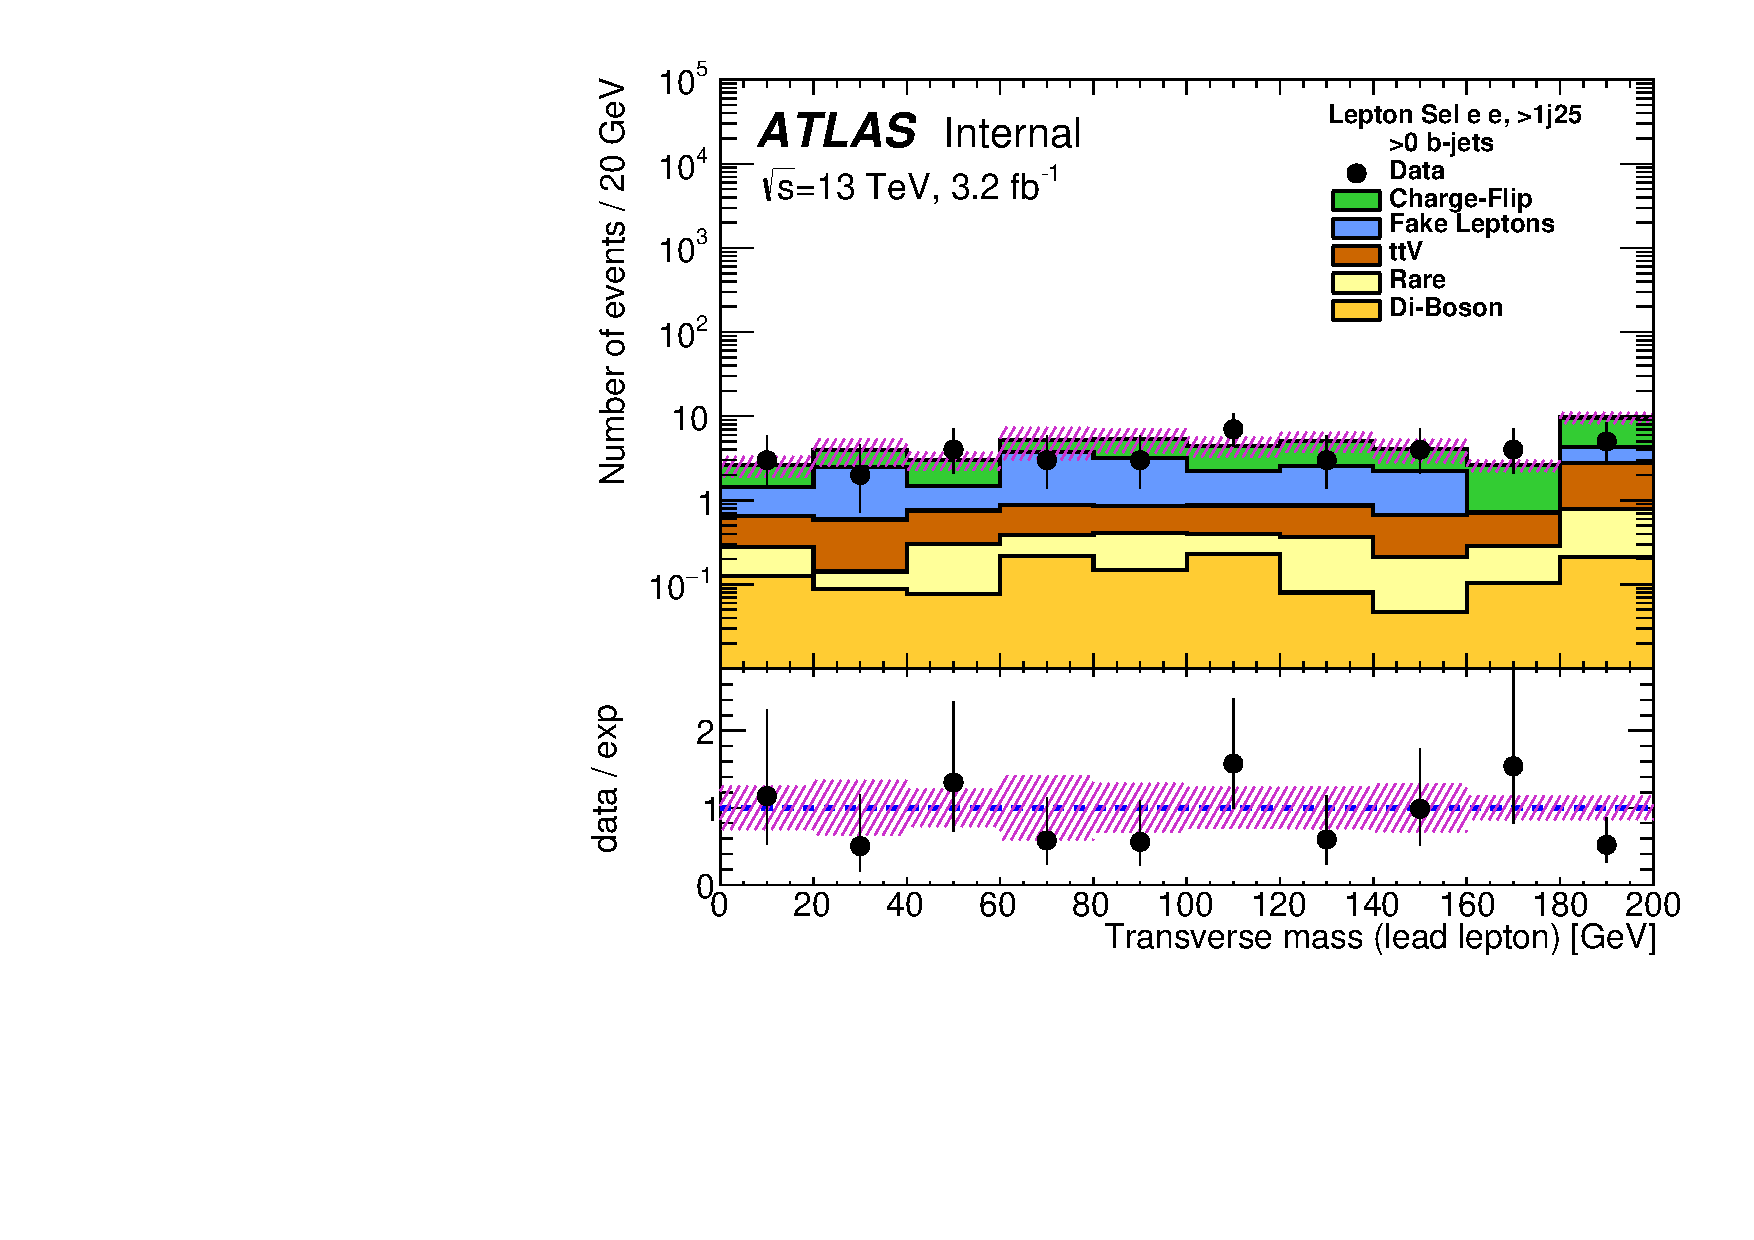
\includegraphics[width=0.45\textwidth]{BKG/validationPLots/MT_EE_LEP}
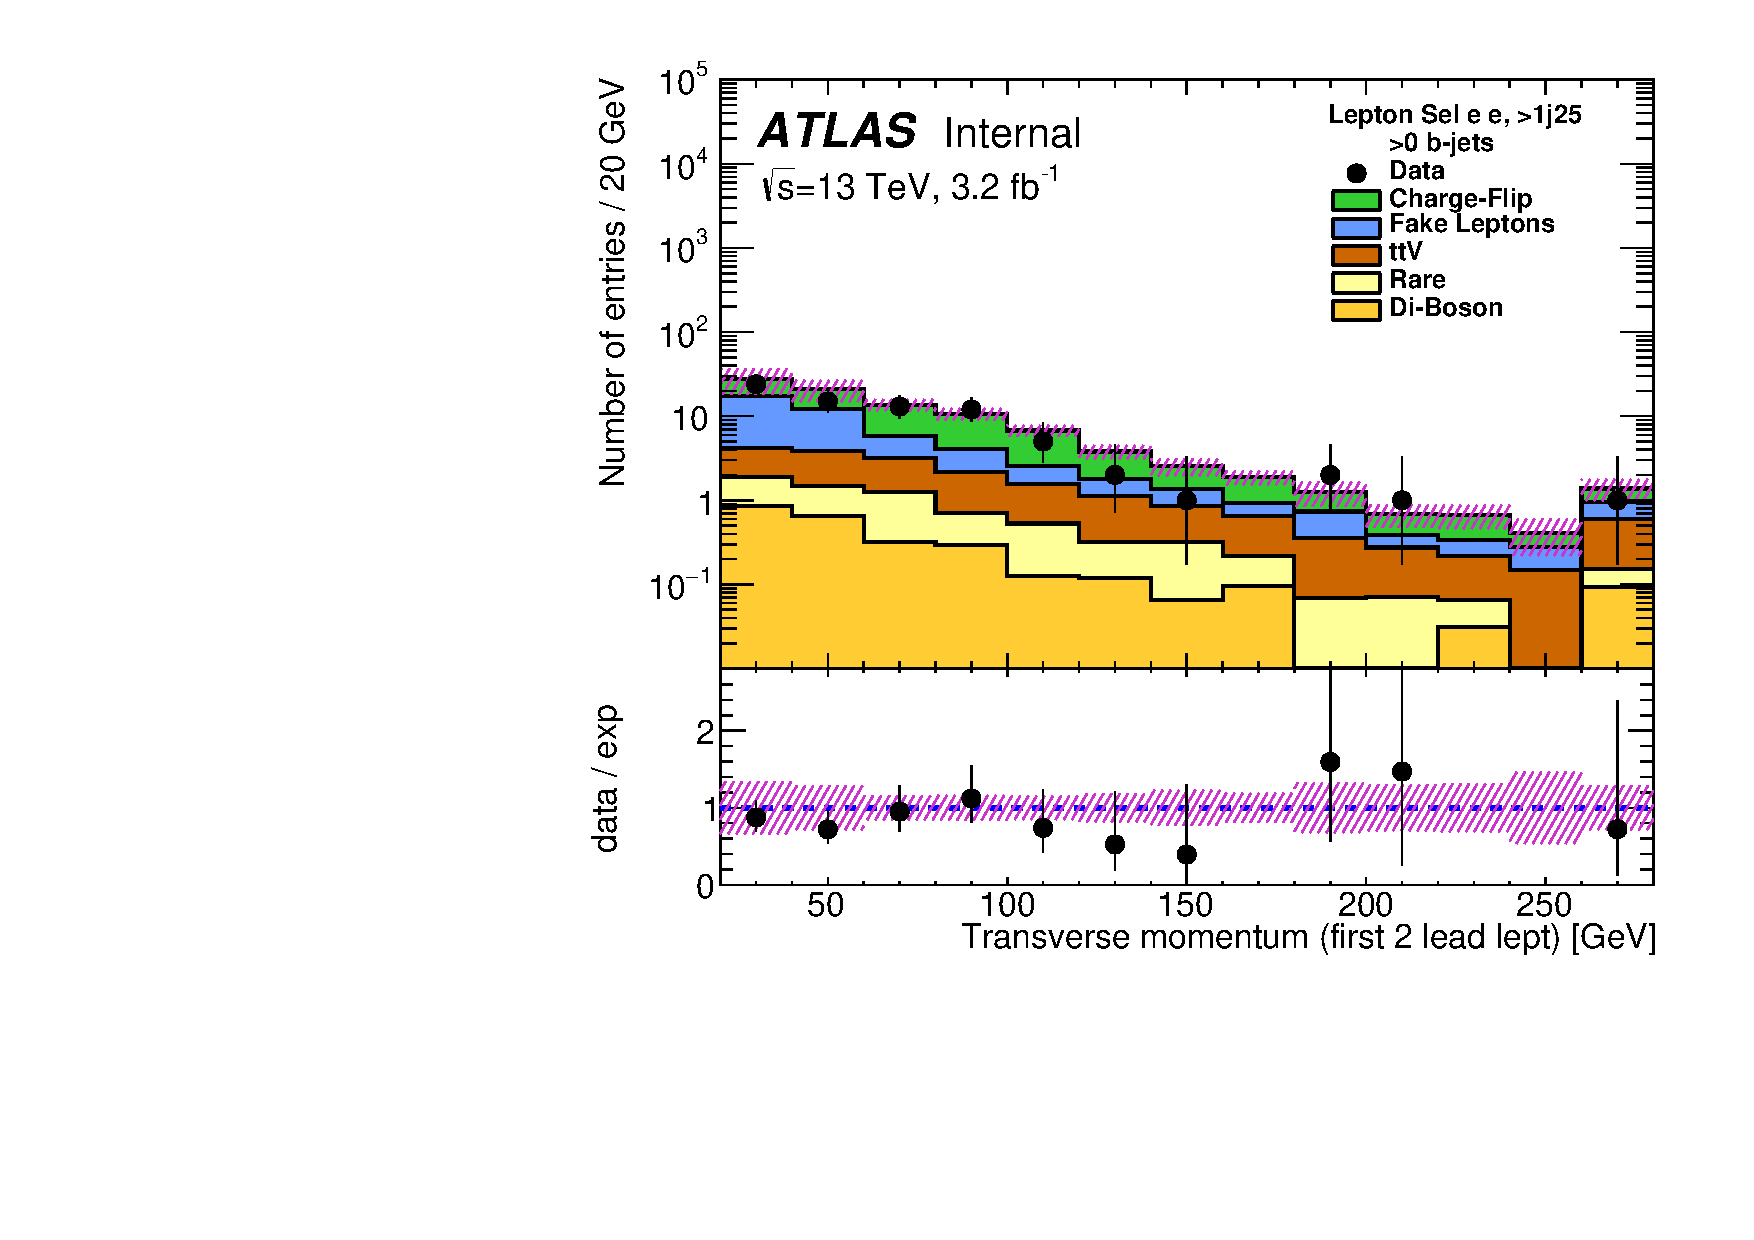
\includegraphics[width=0.45\textwidth]{BKG/validationPLots/PTLEP_EE_LEP}
}
\subfigure{
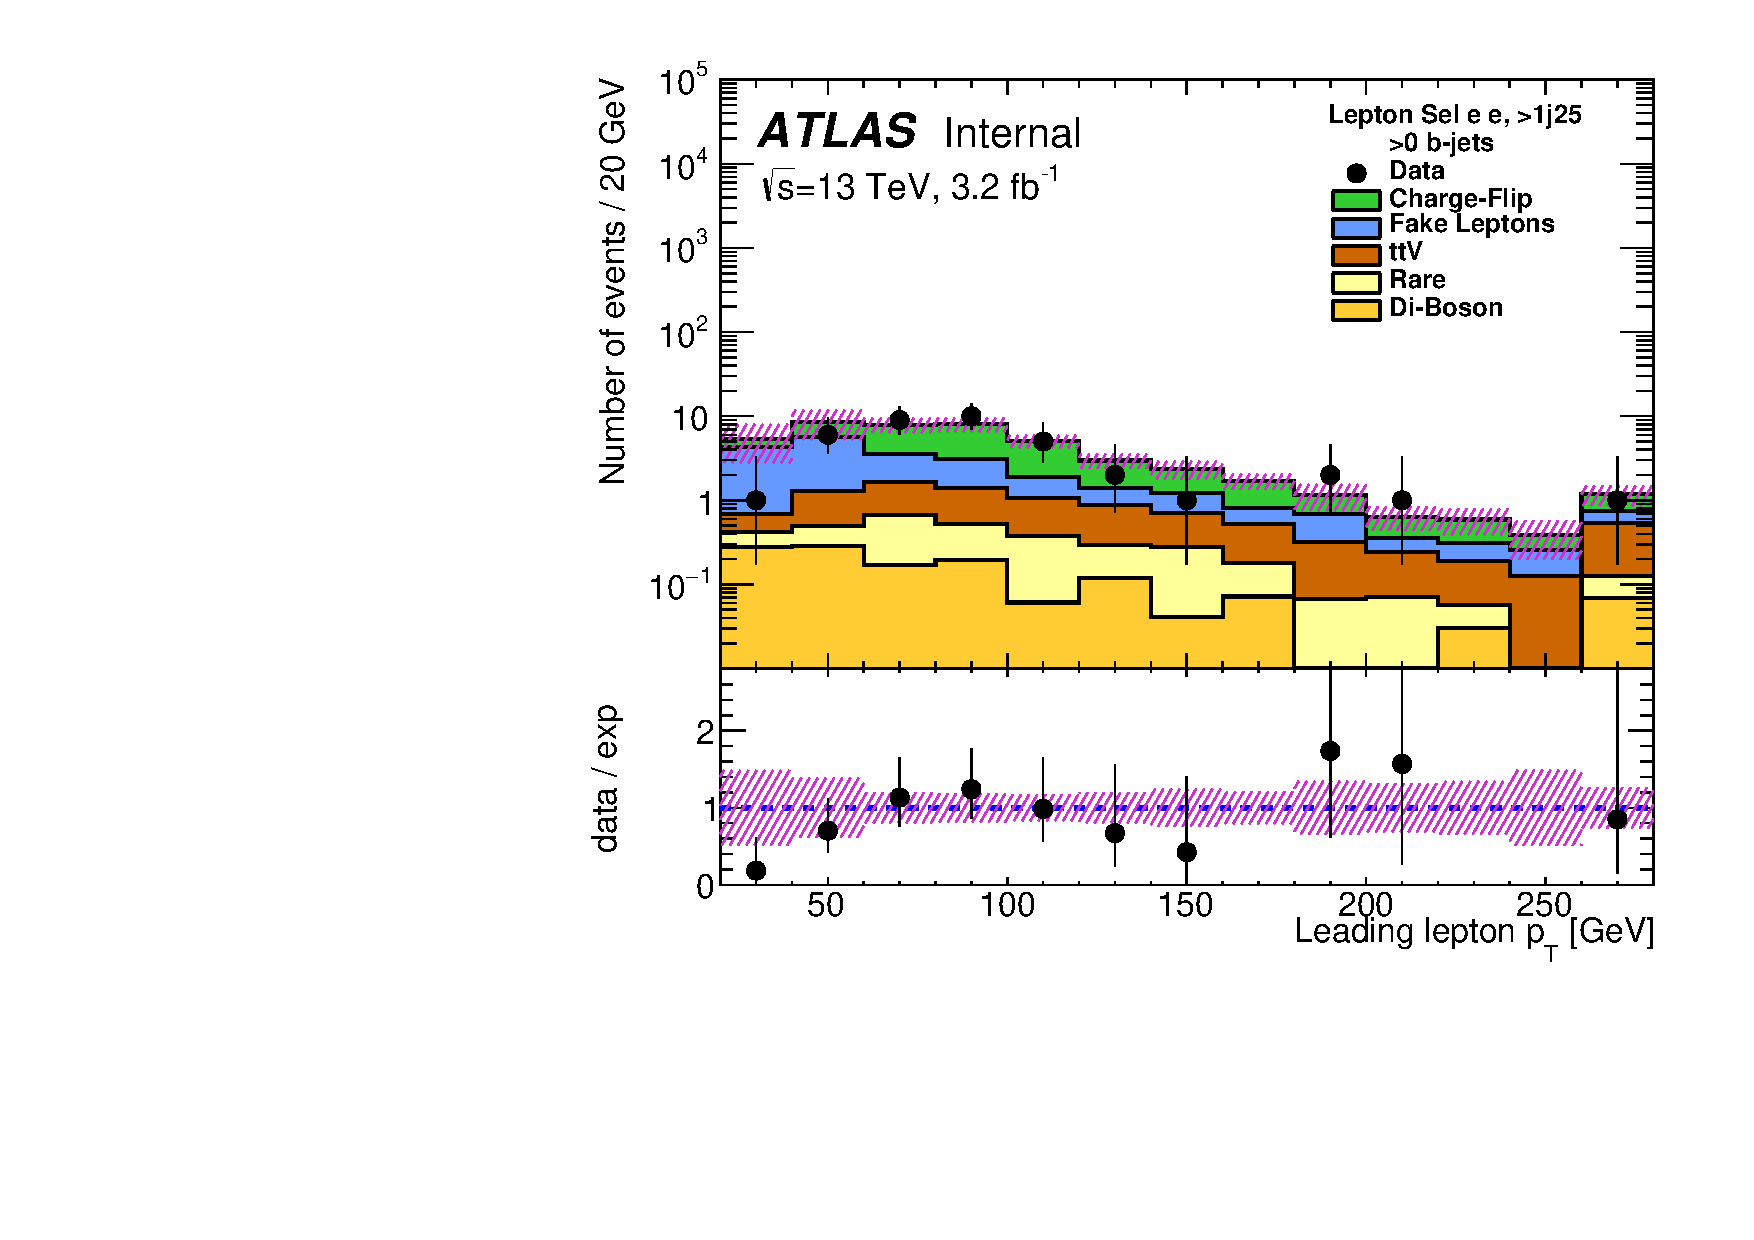
\includegraphics[width=0.45\textwidth]{BKG/validationPLots/PTLEP_EE_LEAD}
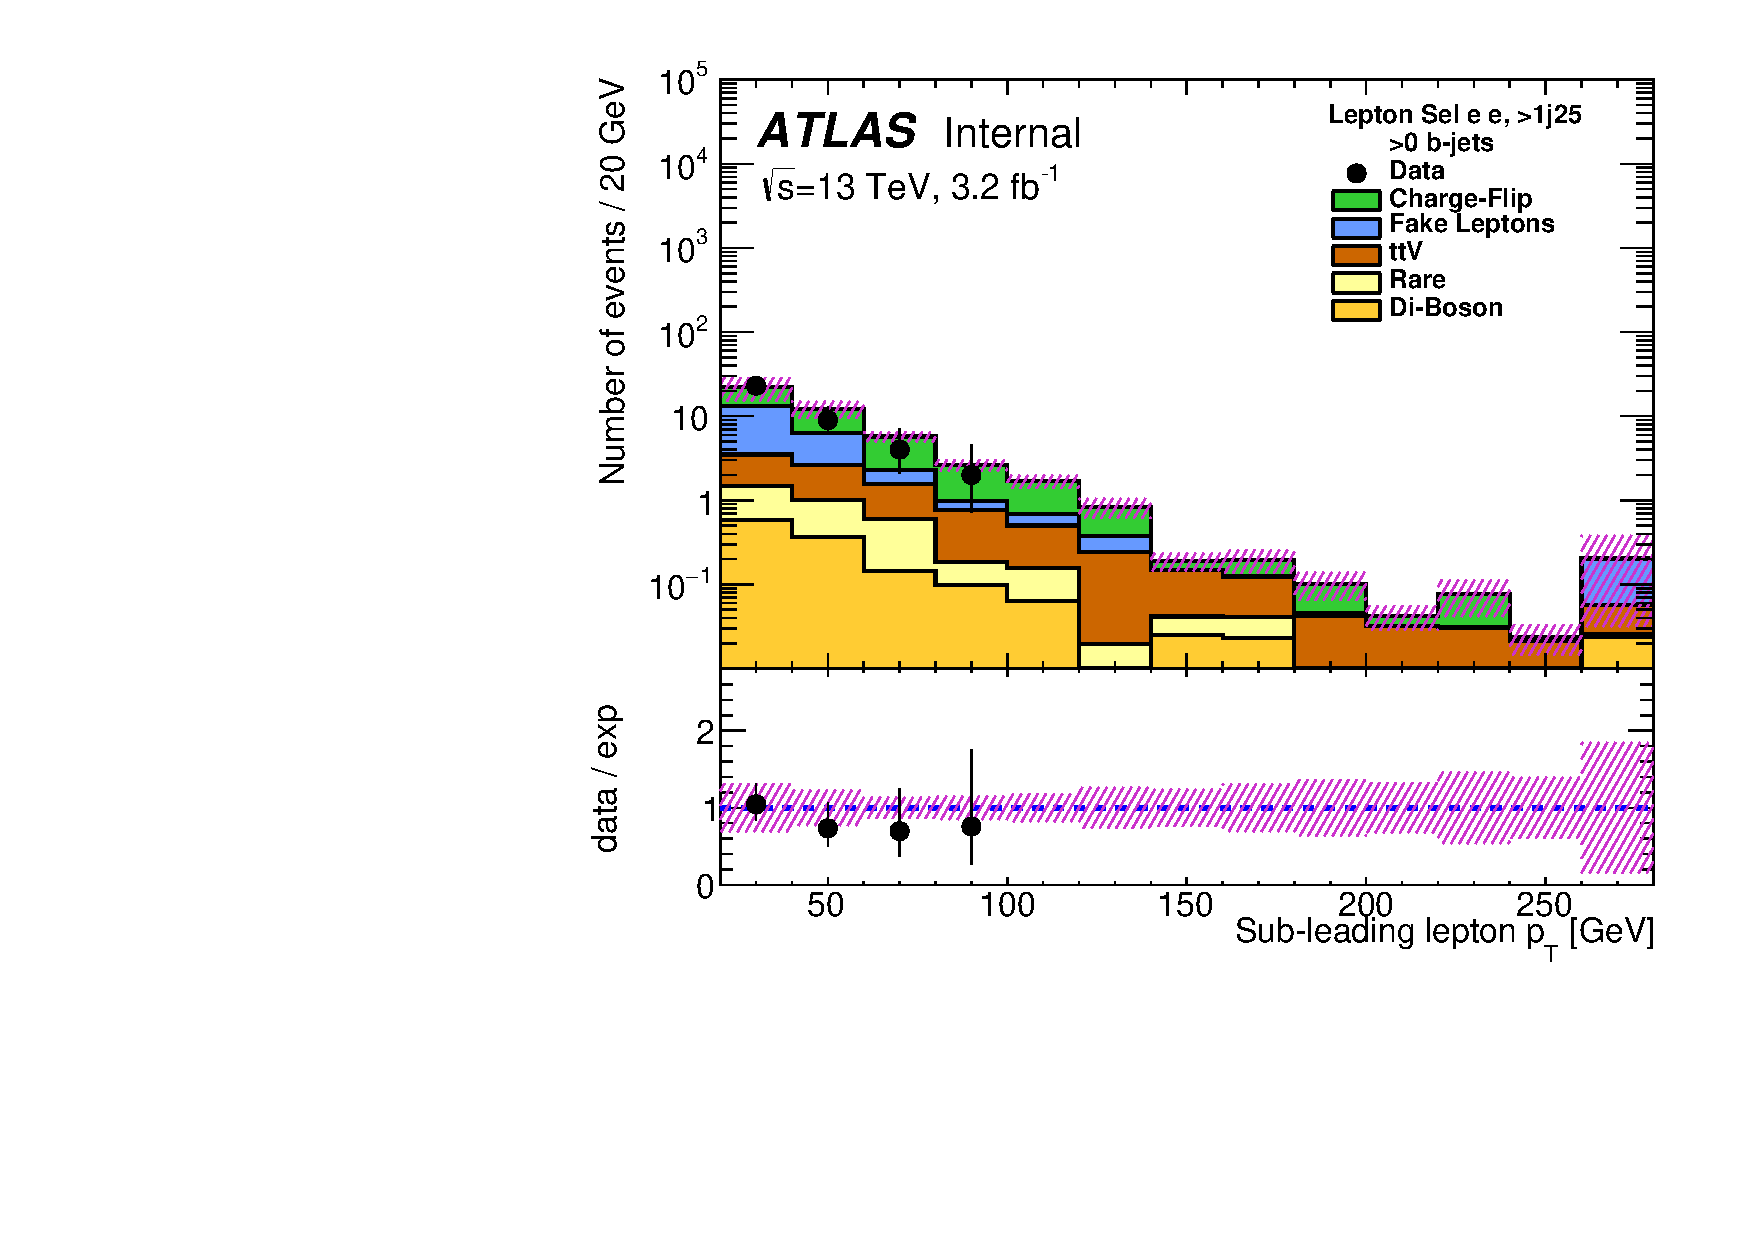
\includegraphics[width=0.45\textwidth]{BKG/validationPLots/PTLEP_EE_SUBLEAD}
}
\caption{$ee$ channel, \met $>$ 60\GeV and $N_{jets}^{25}$~$\ge$2: Distributions of  jet multiplicity (\pt~$>$~25~GeV) (top-left) and $b$-jet multiplicity (\pt~$>$~20~GeV) (top-right) after lepton selection, and of \mt (middle-left), selected leptons \pt (middle-right), leading lepton \pt (bottom-left) and subleading lepton \pt (bottom-right) after lepton selections with at least one $b$-jet (\pt~$>$~20~GeV).}
\label{Fig:VP_ee_1b_Njets_and_other}
\end{figure} 




%%%%% ee channel, ==0 b-jet
\begin{figure}[h!]
\centering
\subfigure{
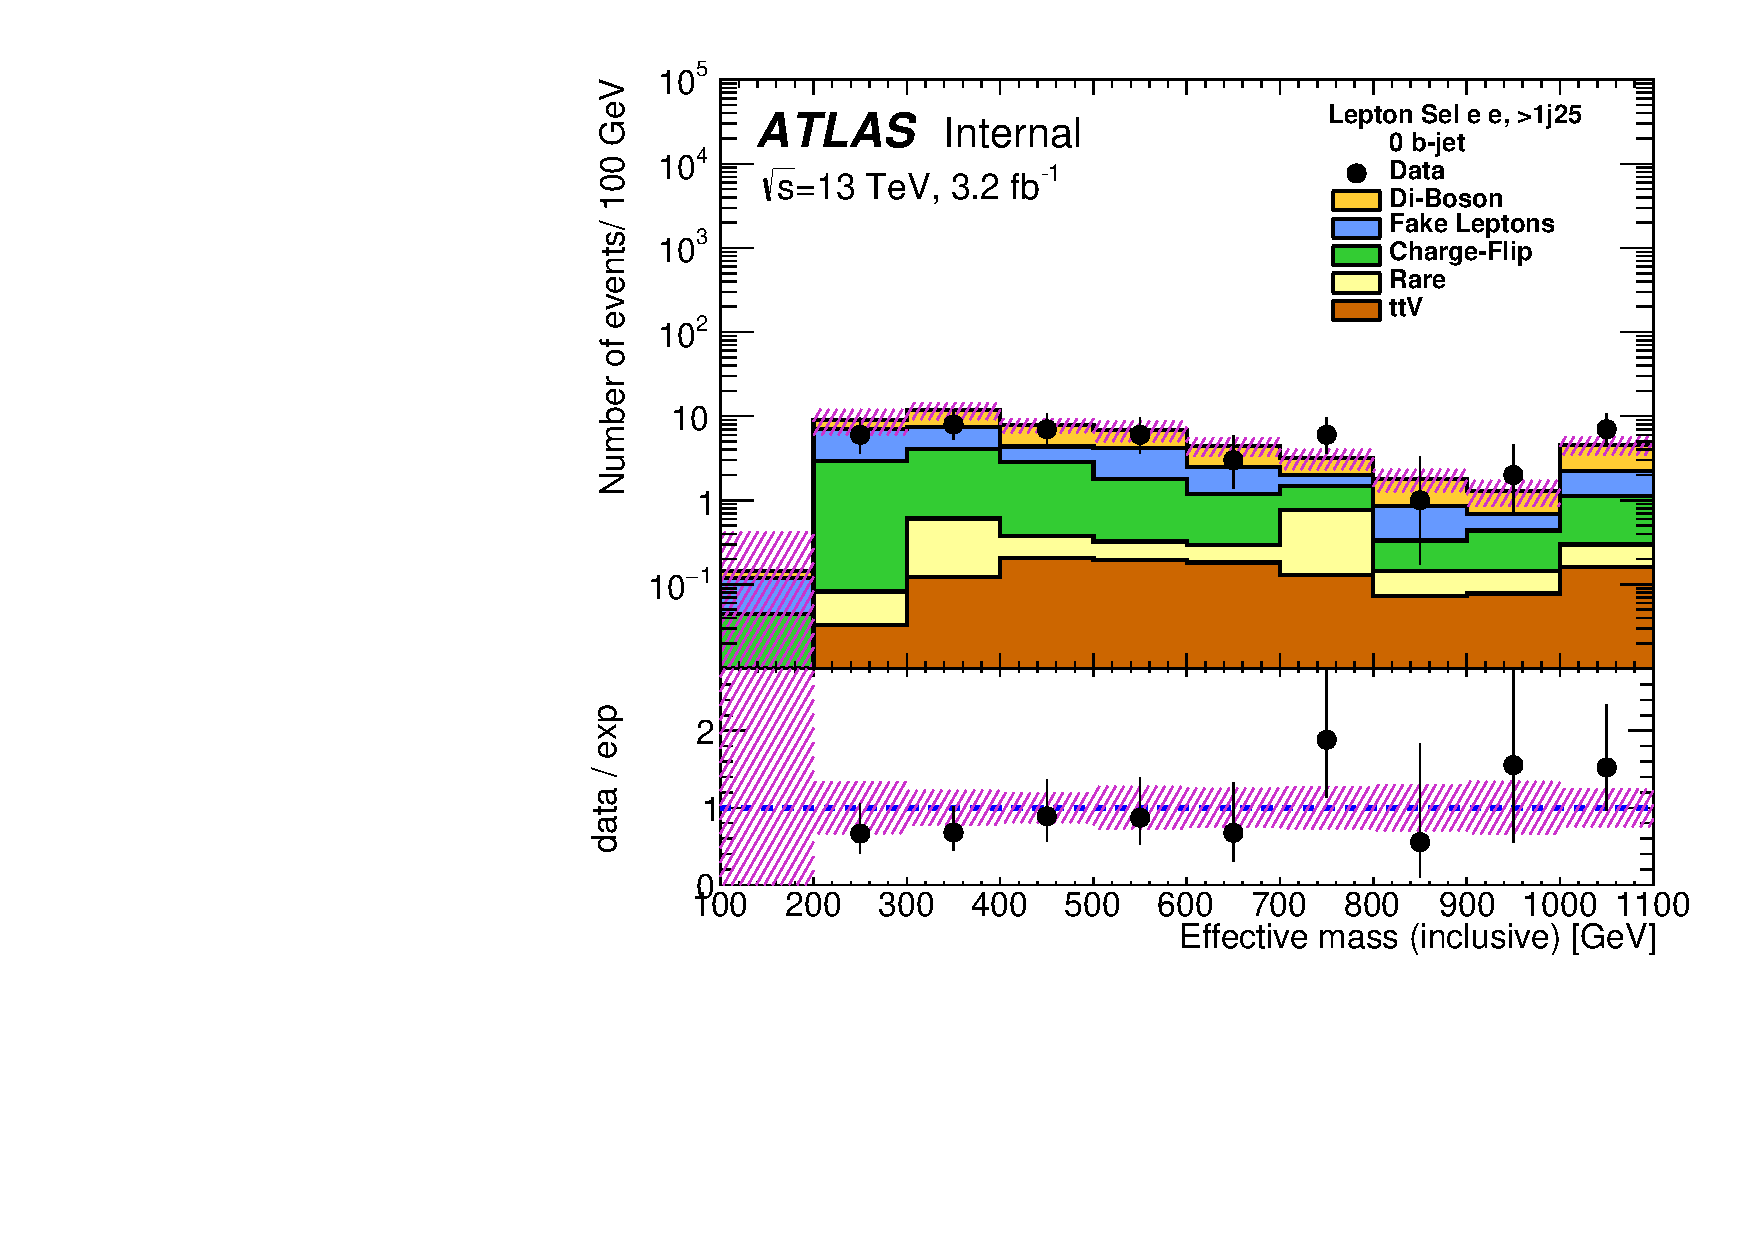
\includegraphics[width=0.5\textwidth]{BKG/validationPLots/MEFF_EE_BVETOLEP}
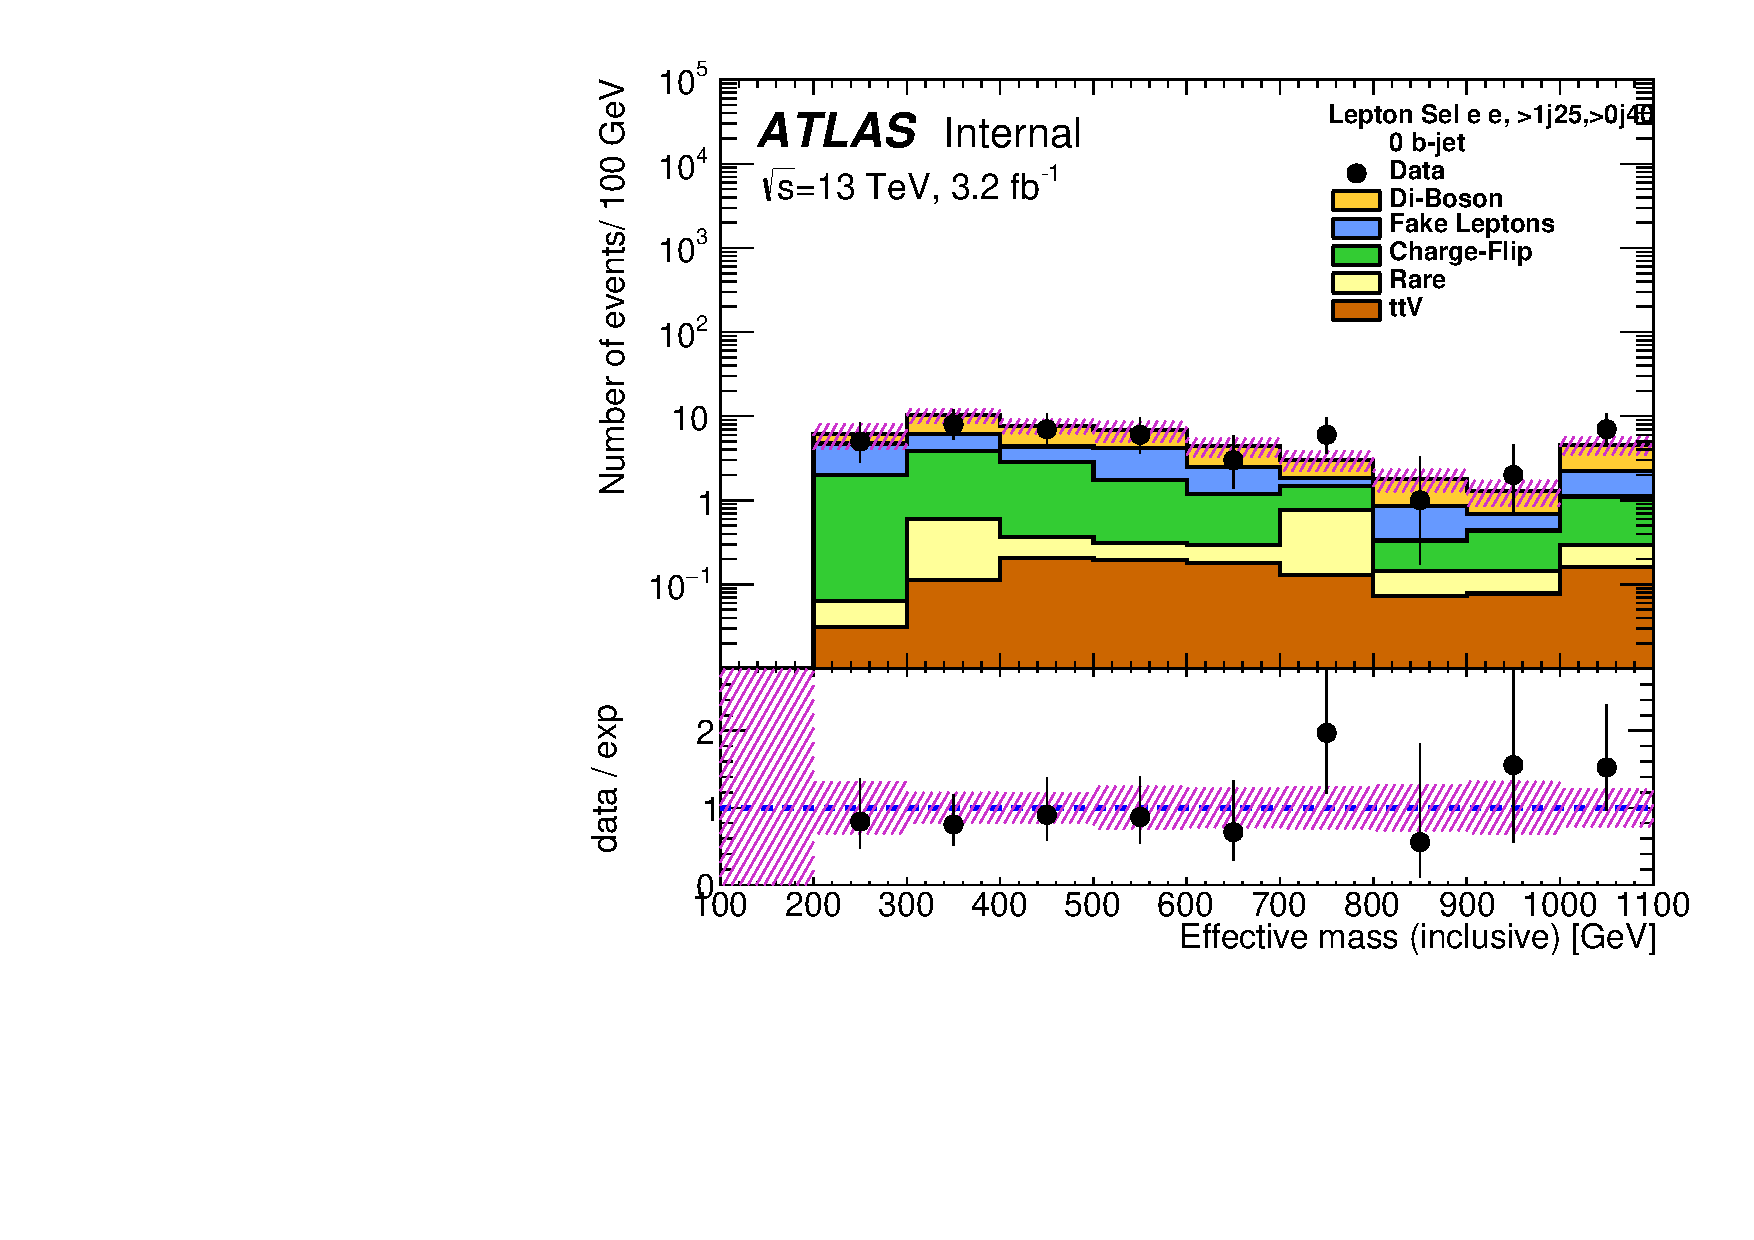
\includegraphics[width=0.5\textwidth]{BKG/validationPLots/MEFF_EE_BVETOL1JET}
}
\subfigure{
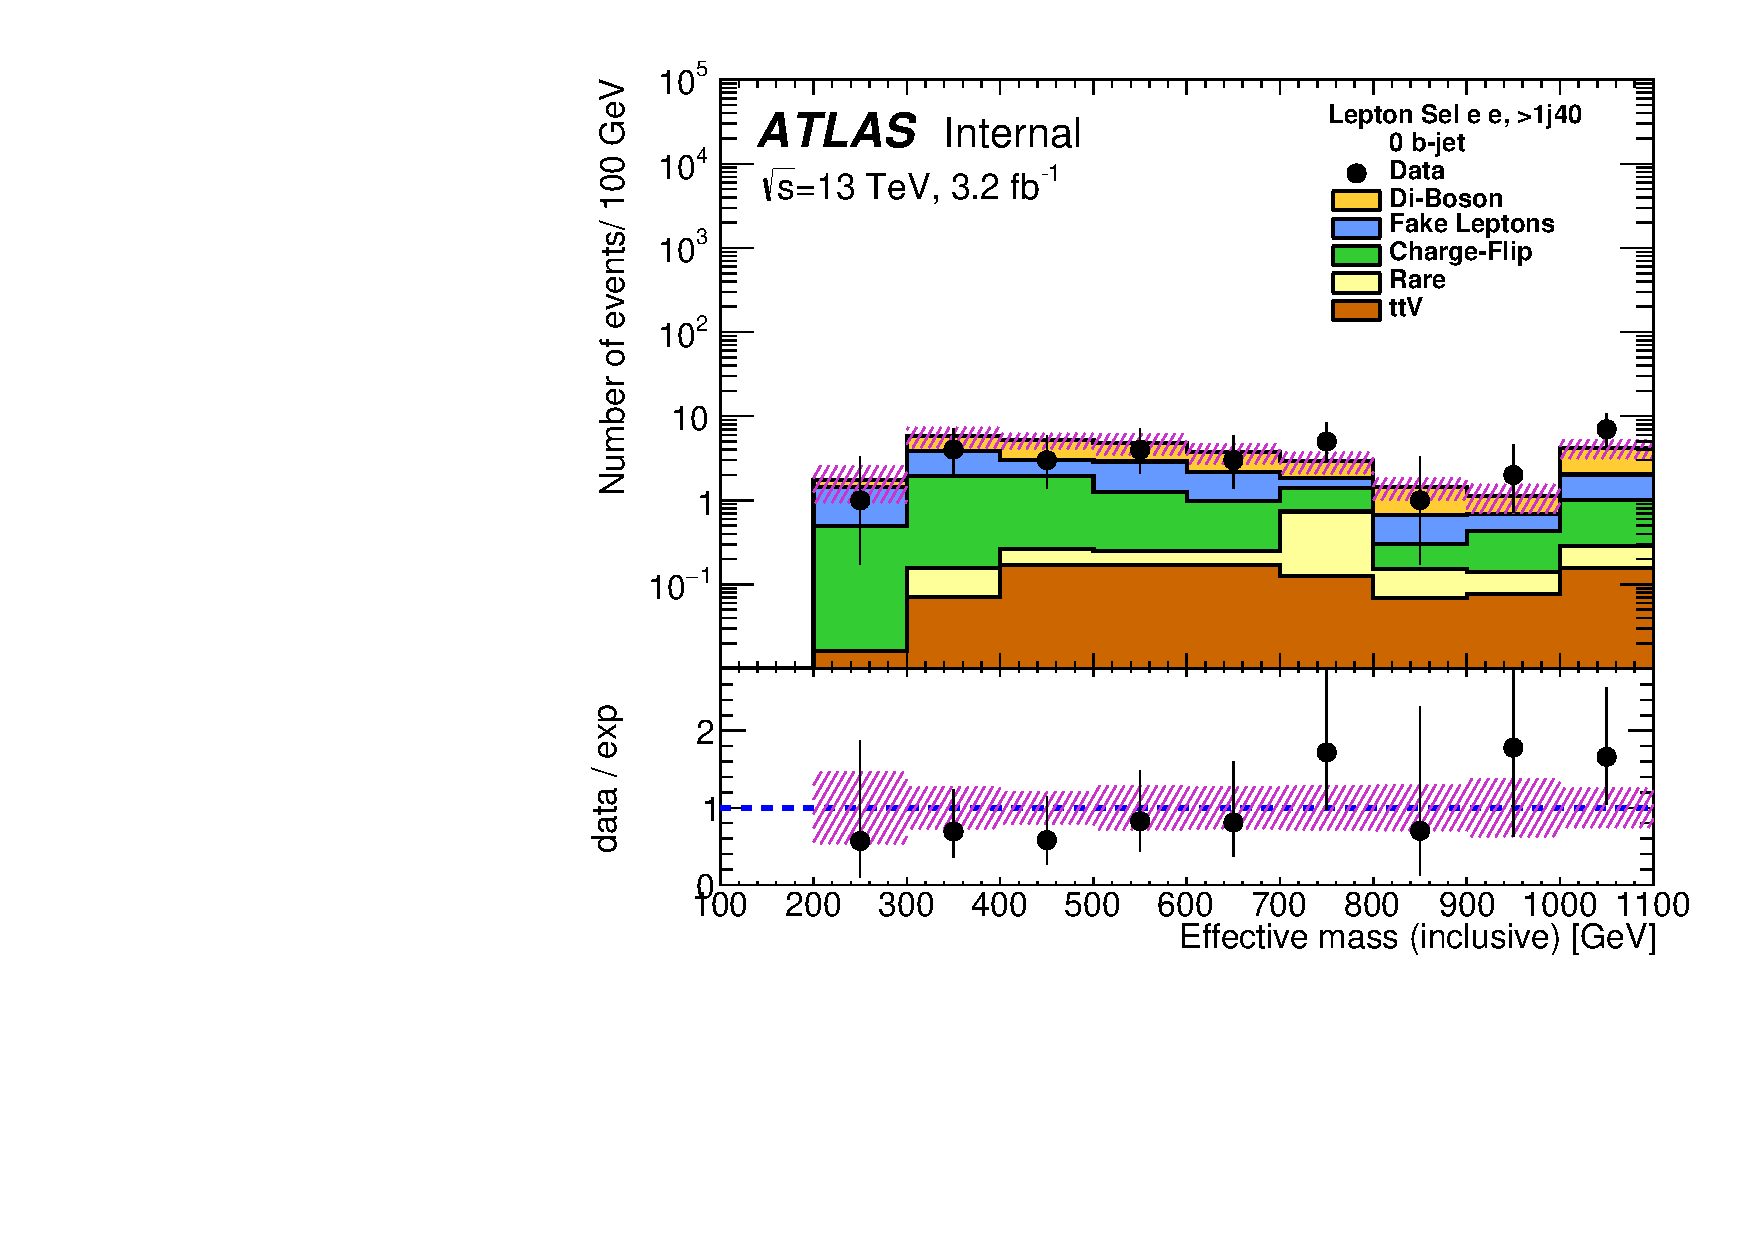
\includegraphics[width=0.5\textwidth]{BKG/validationPLots/MEFF_EE_BVETOL2JET}
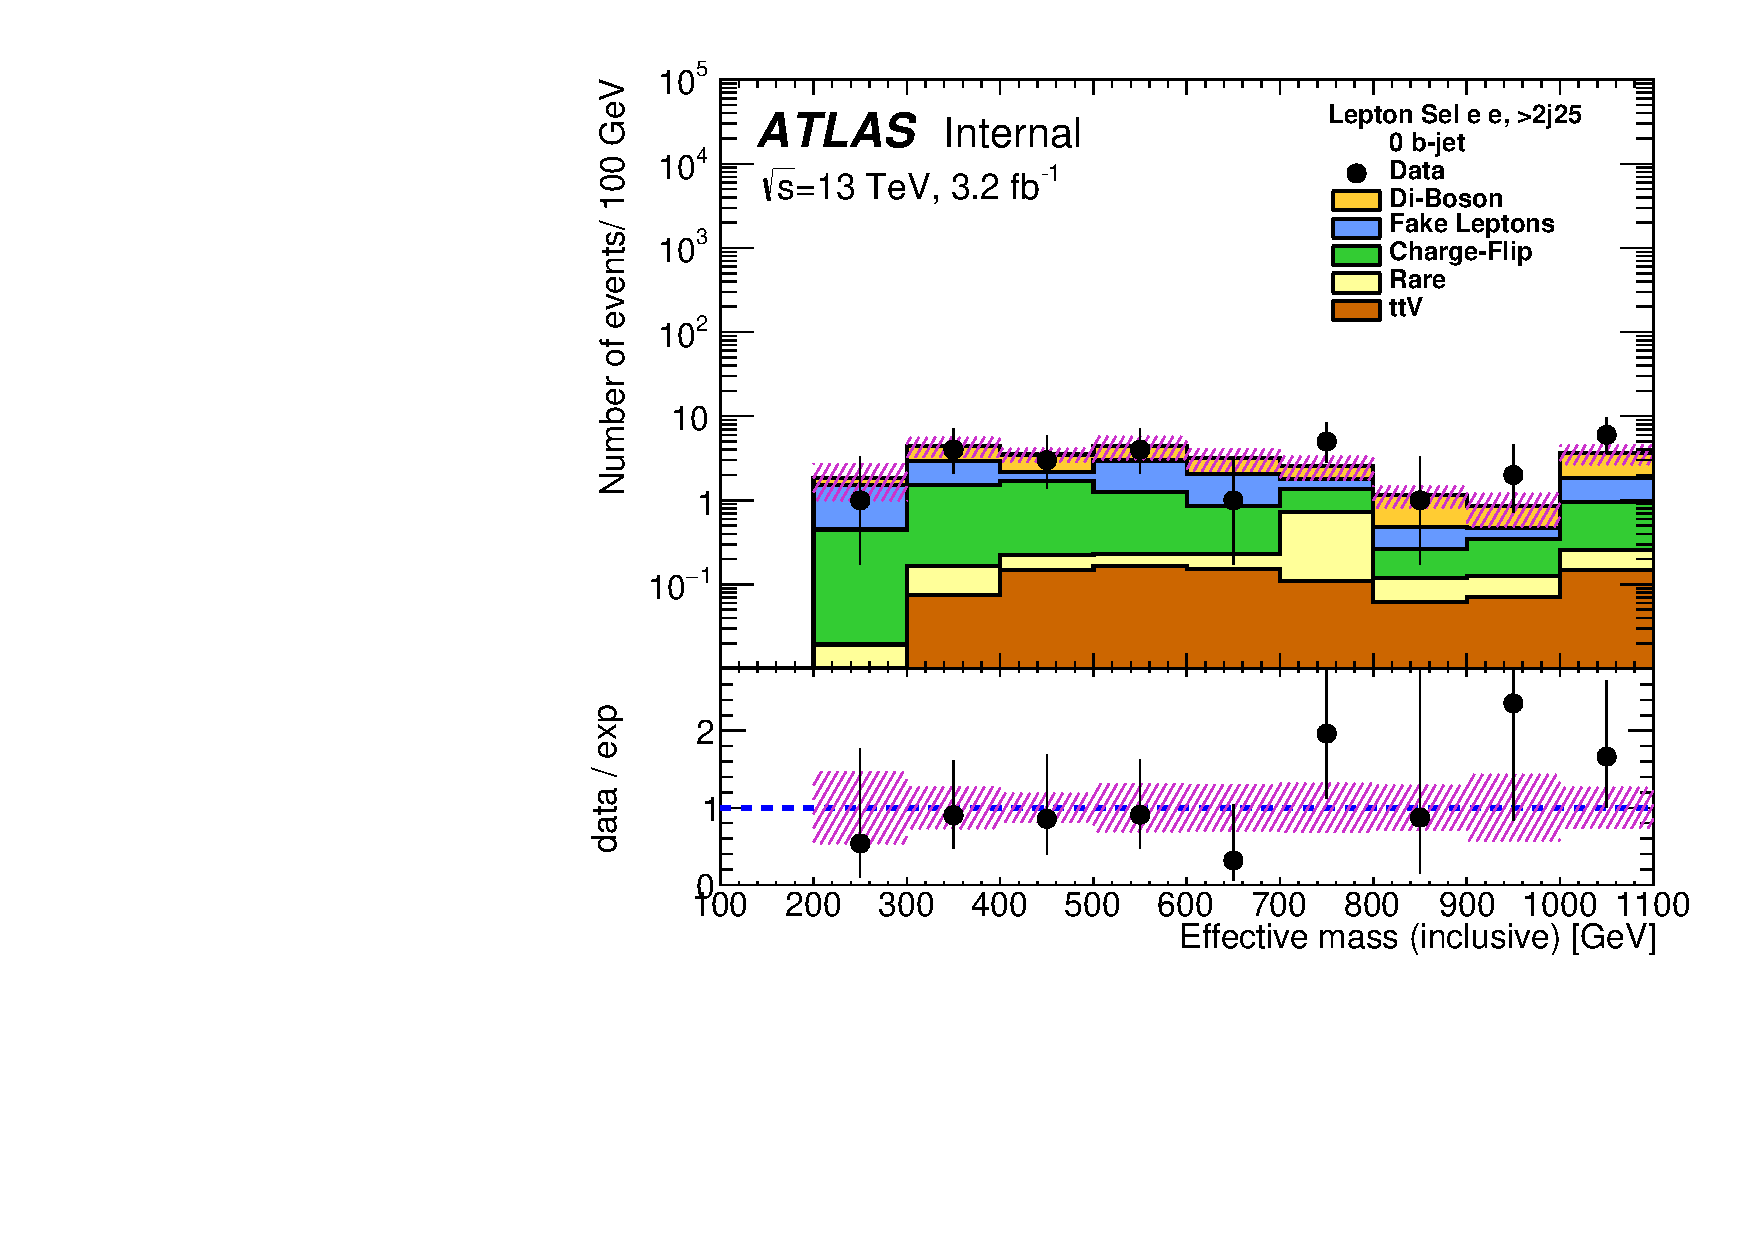
\includegraphics[width=0.5\textwidth]{BKG/validationPLots/MEFF_EE_BVETOL3JET}
}
\caption{$ee$ channel, \met $>$ 60\GeV and $N_{jets}^{25}$~$\ge$2: Effective mass distribution after lepton selections with a $b$-jet veto (\pt~$>$~20~GeV) and with at least 0, 1, 2 and 3 jets with \pt~$>$~40~GeV (from top-left to bottom-right).}
\label{Fig:VP_ee_0b_Meff}
\end{figure}
%%
\begin{figure}[h!]
\centering
\subfigure{
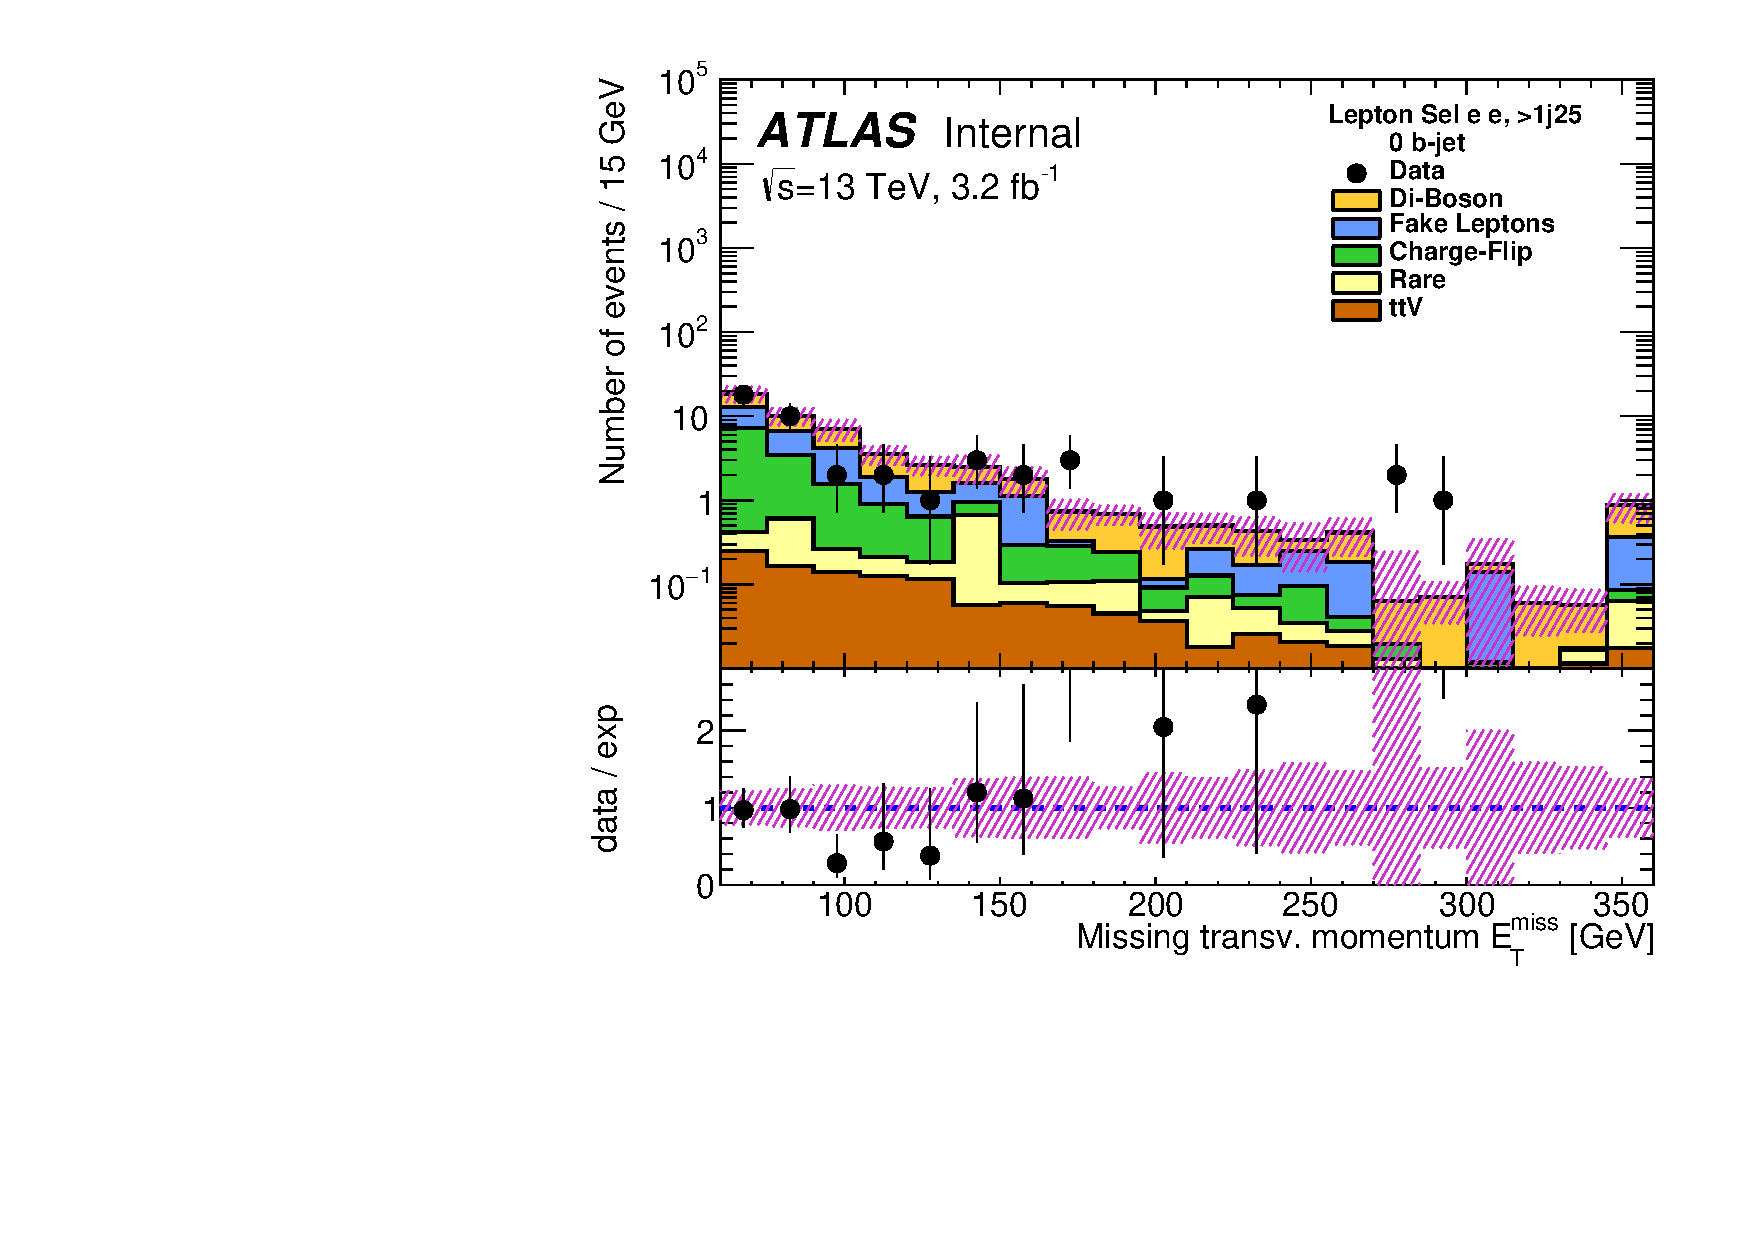
\includegraphics[width=0.5\textwidth]{BKG/validationPLots/MET_EE_BVETOLEP}
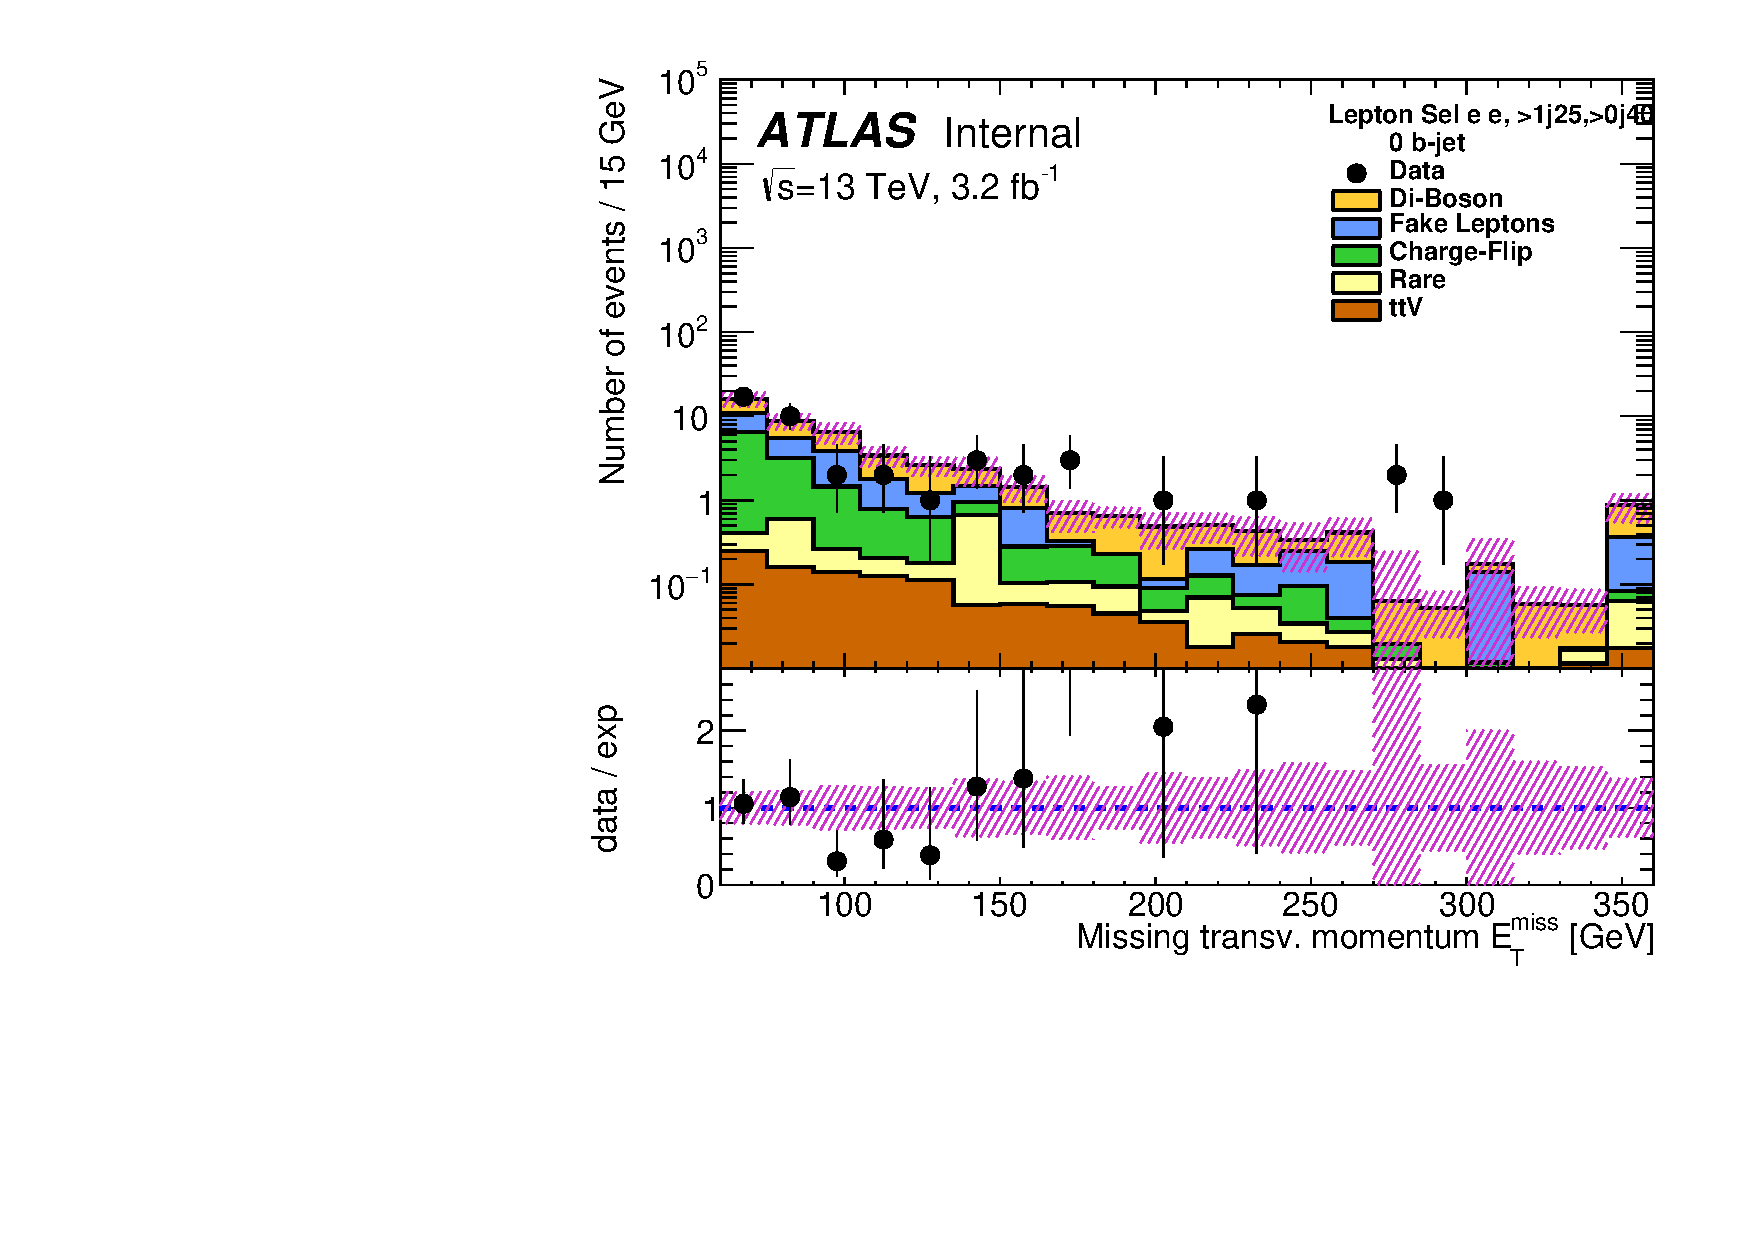
\includegraphics[width=0.5\textwidth]{BKG/validationPLots/MET_EE_BVETOL1JET}
}
\subfigure{
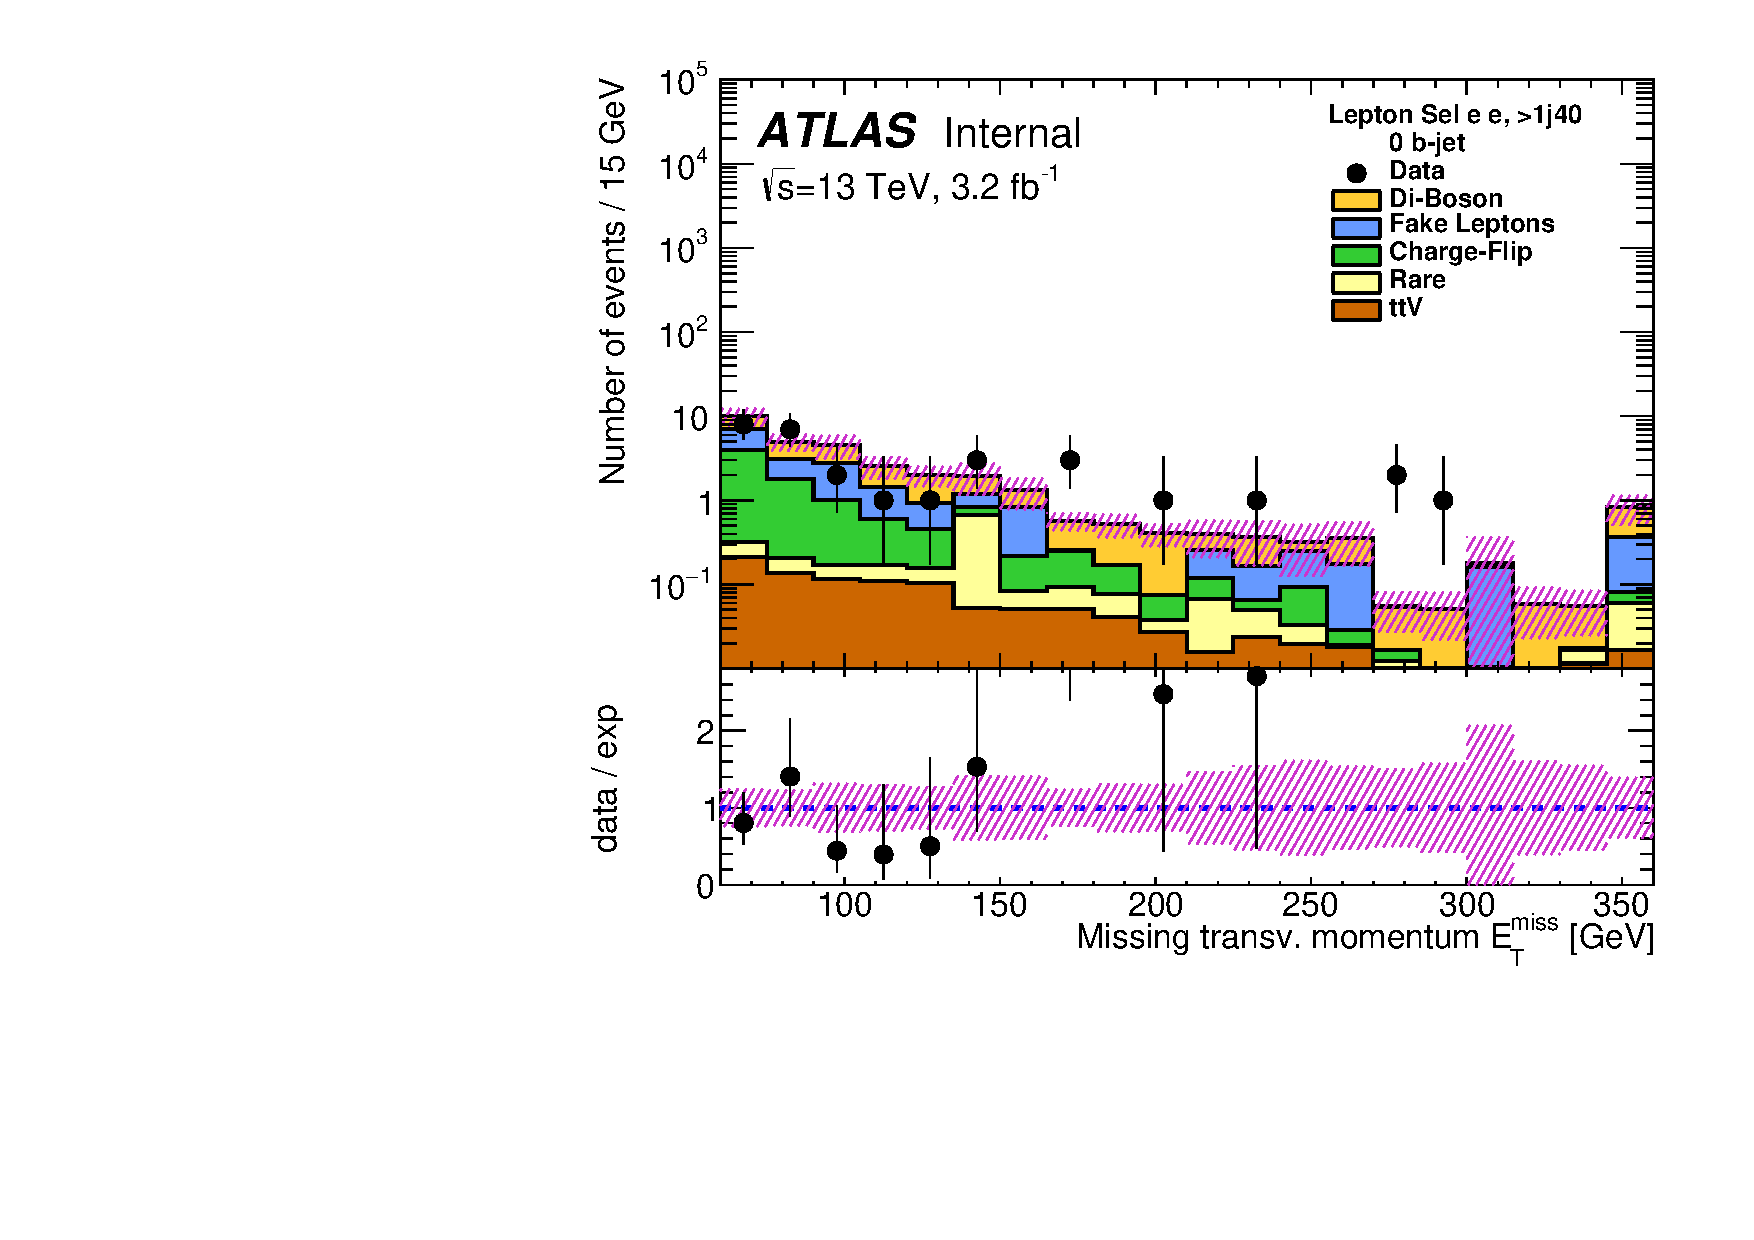
\includegraphics[width=0.5\textwidth]{BKG/validationPLots/MET_EE_BVETOL2JET}
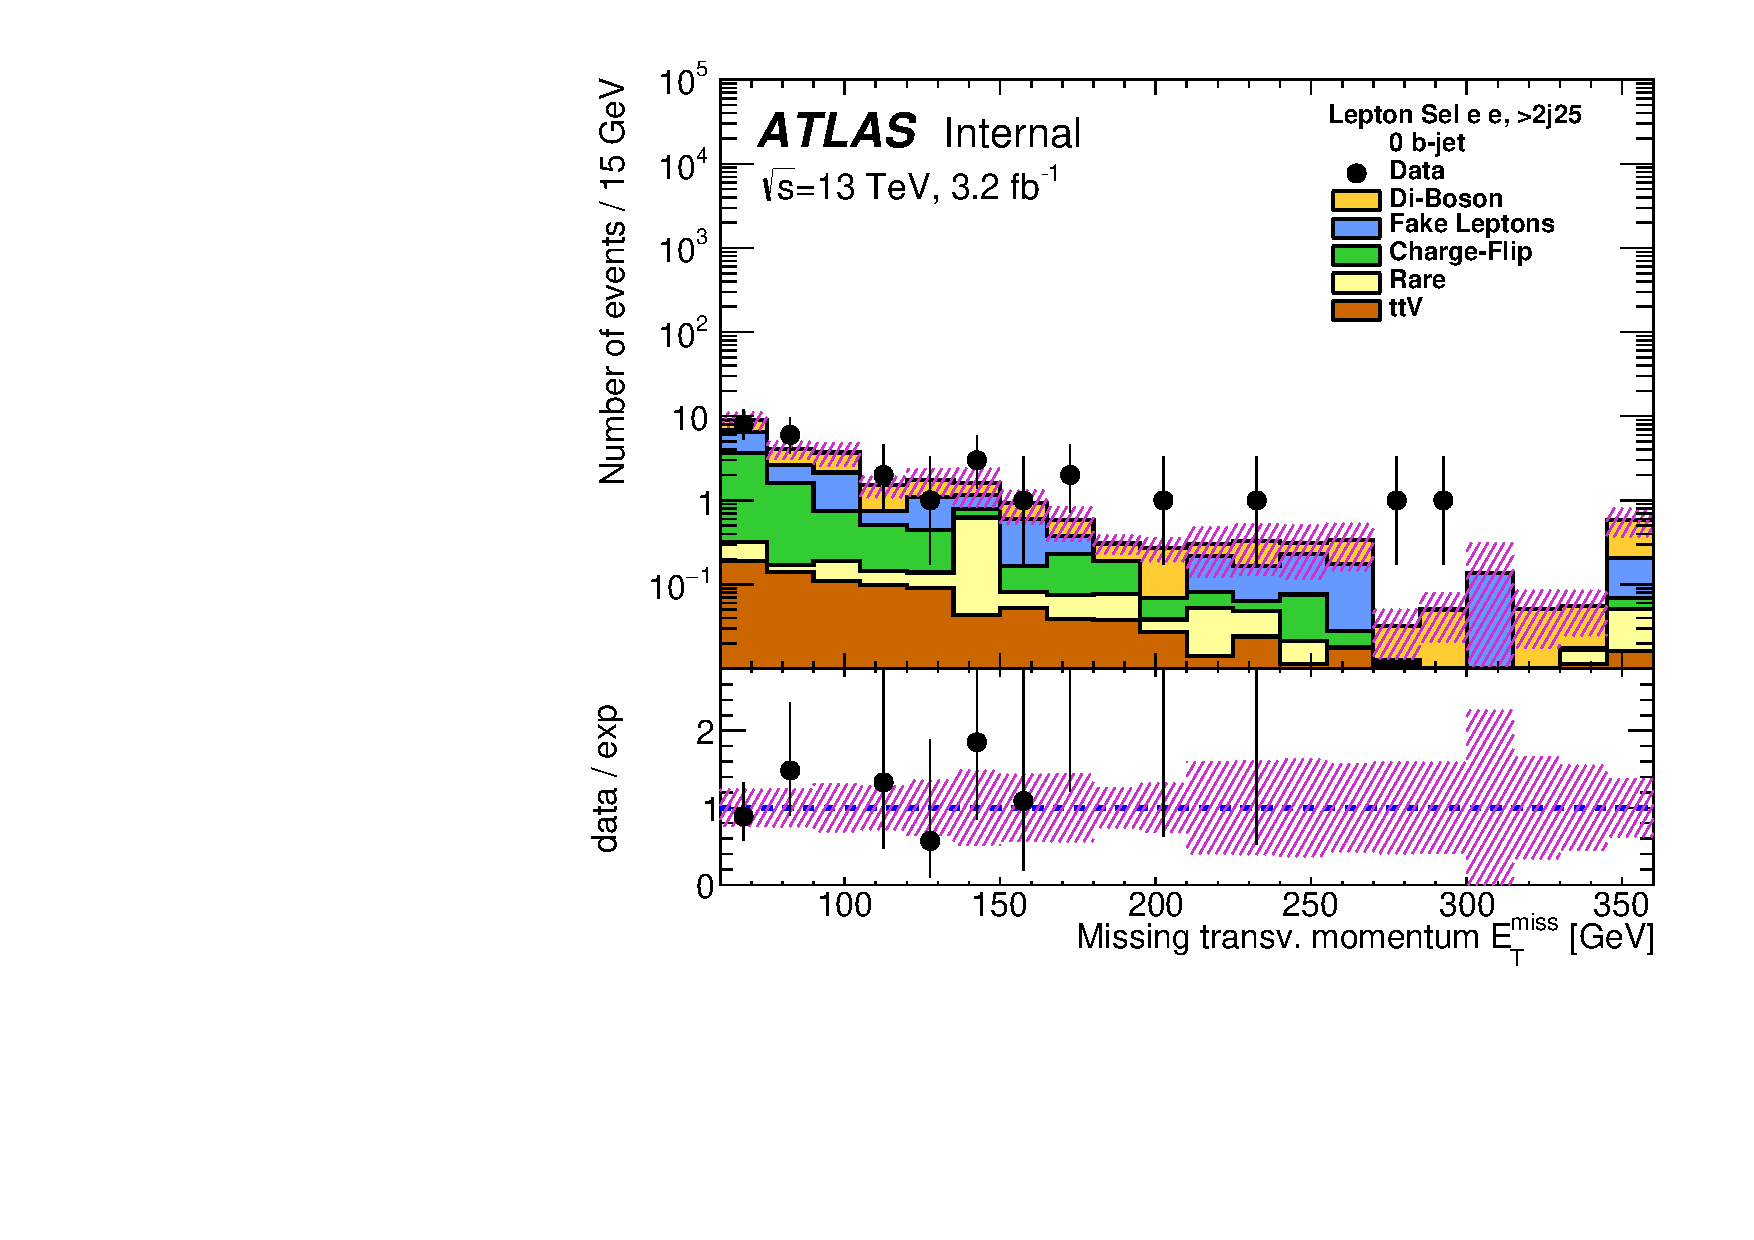
\includegraphics[width=0.5\textwidth]{BKG/validationPLots/MET_EE_BVETOL3JET}
}
\caption{$ee$ channel, \met $>$ 60\GeV and $N_{jets}^{25}$~$\ge$2: Missing transverse energy distribution after lepton selections with a $b$-jet veto (\pt~$>$~20~GeV) and with at least 0, 1, 2 and 3 jets with \pt~$>$~40~GeV (from top-left to bottom-right).}
\label{Fig:VP_ee_0b_Met}
\end{figure}
%%
\begin{figure}[h!]
\centering
\subfigure{
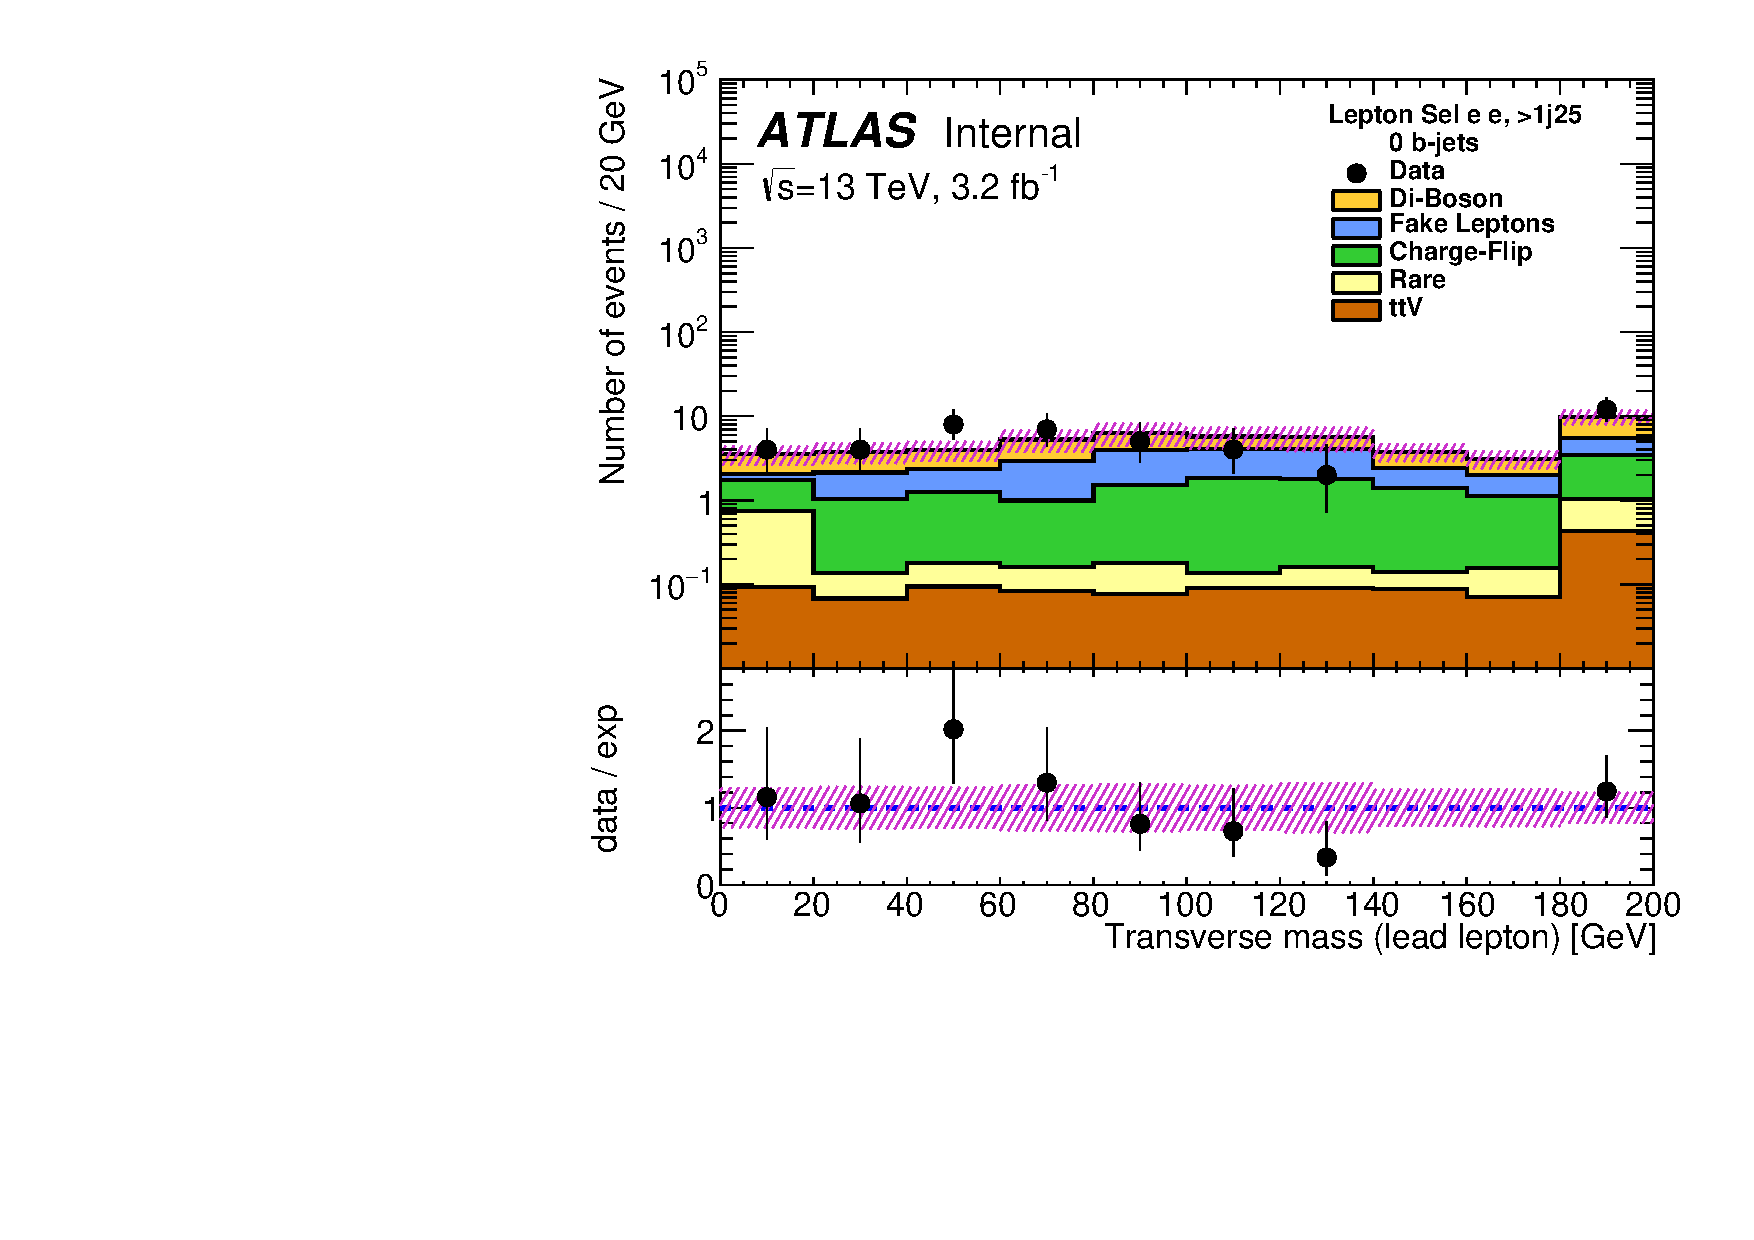
\includegraphics[width=0.5\textwidth]{BKG/validationPLots/MT_EE_BVETOLEP}
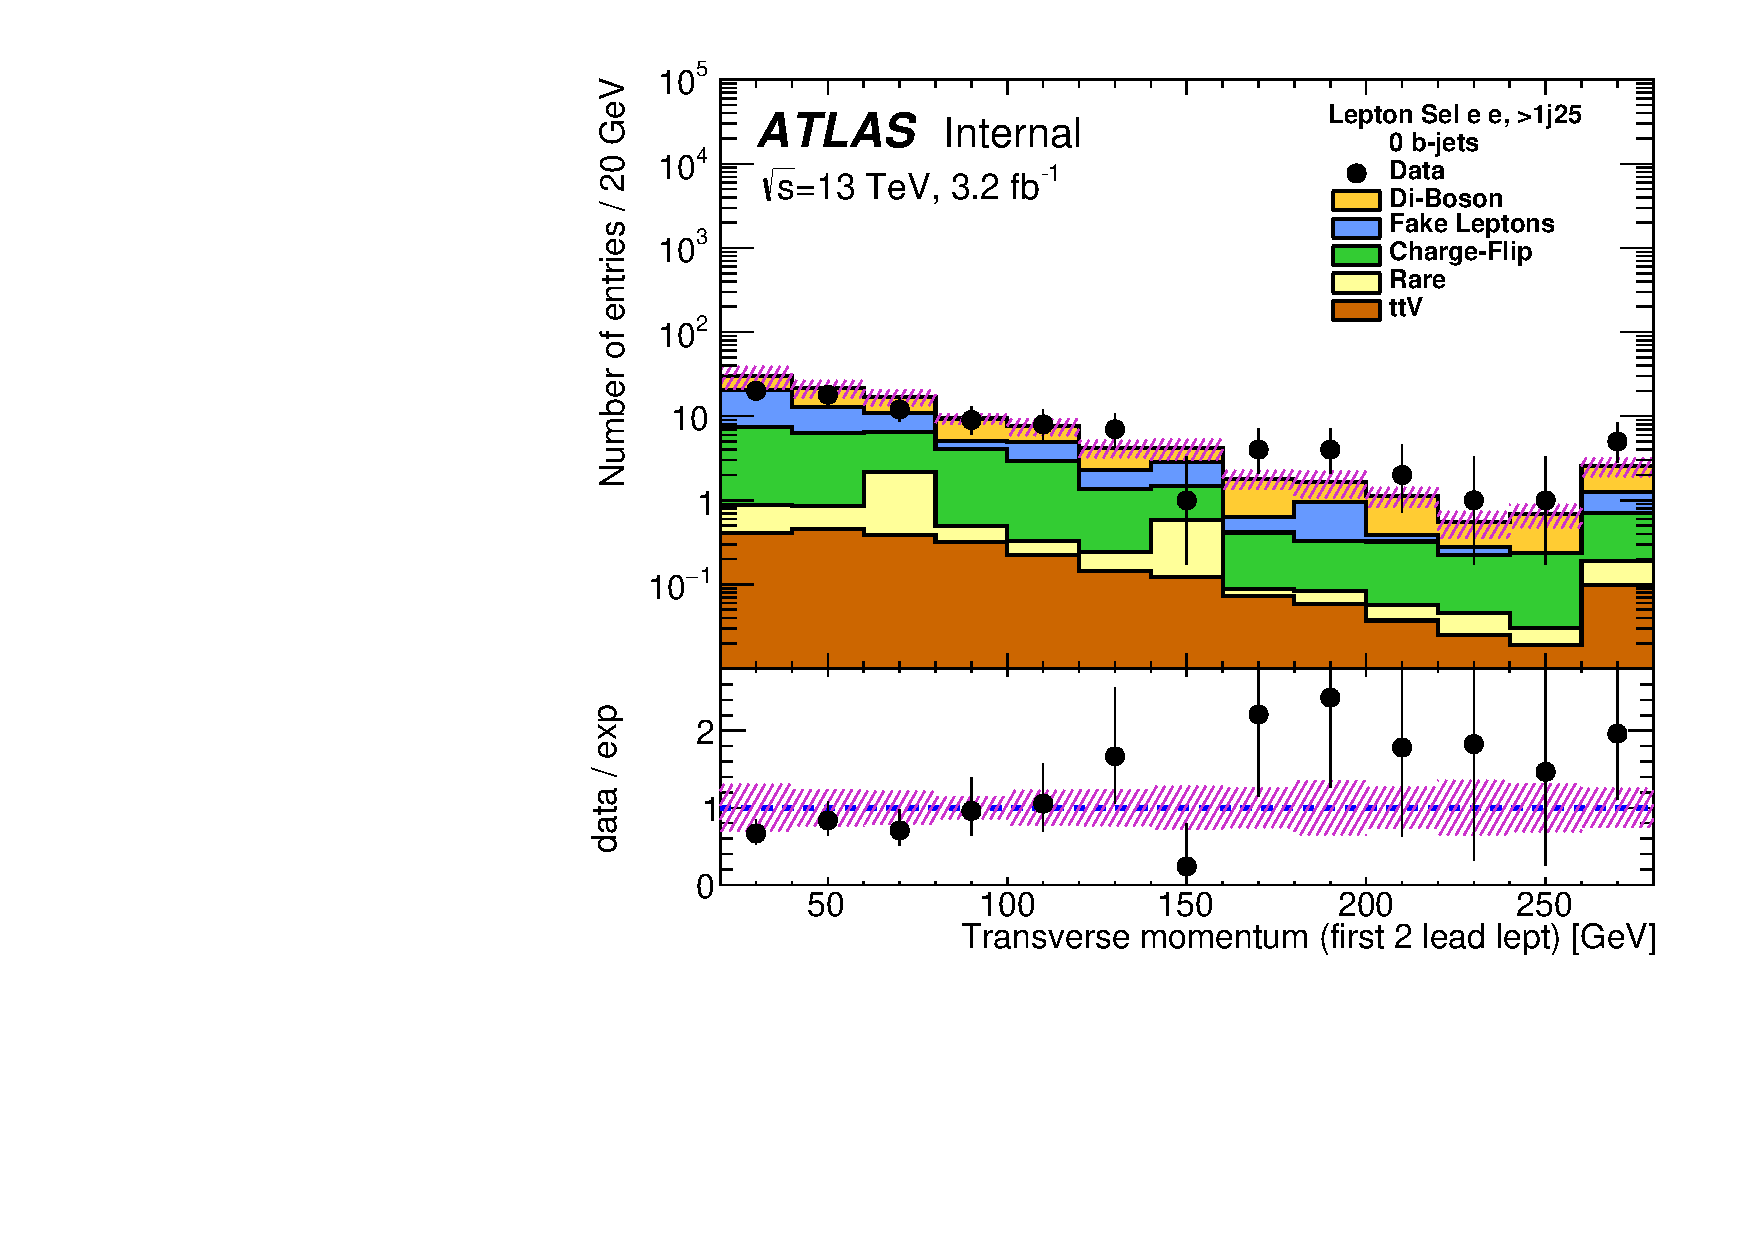
\includegraphics[width=0.5\textwidth]{BKG/validationPLots/PTLEP_EE_BVETOLEP}
}
\subfigure{
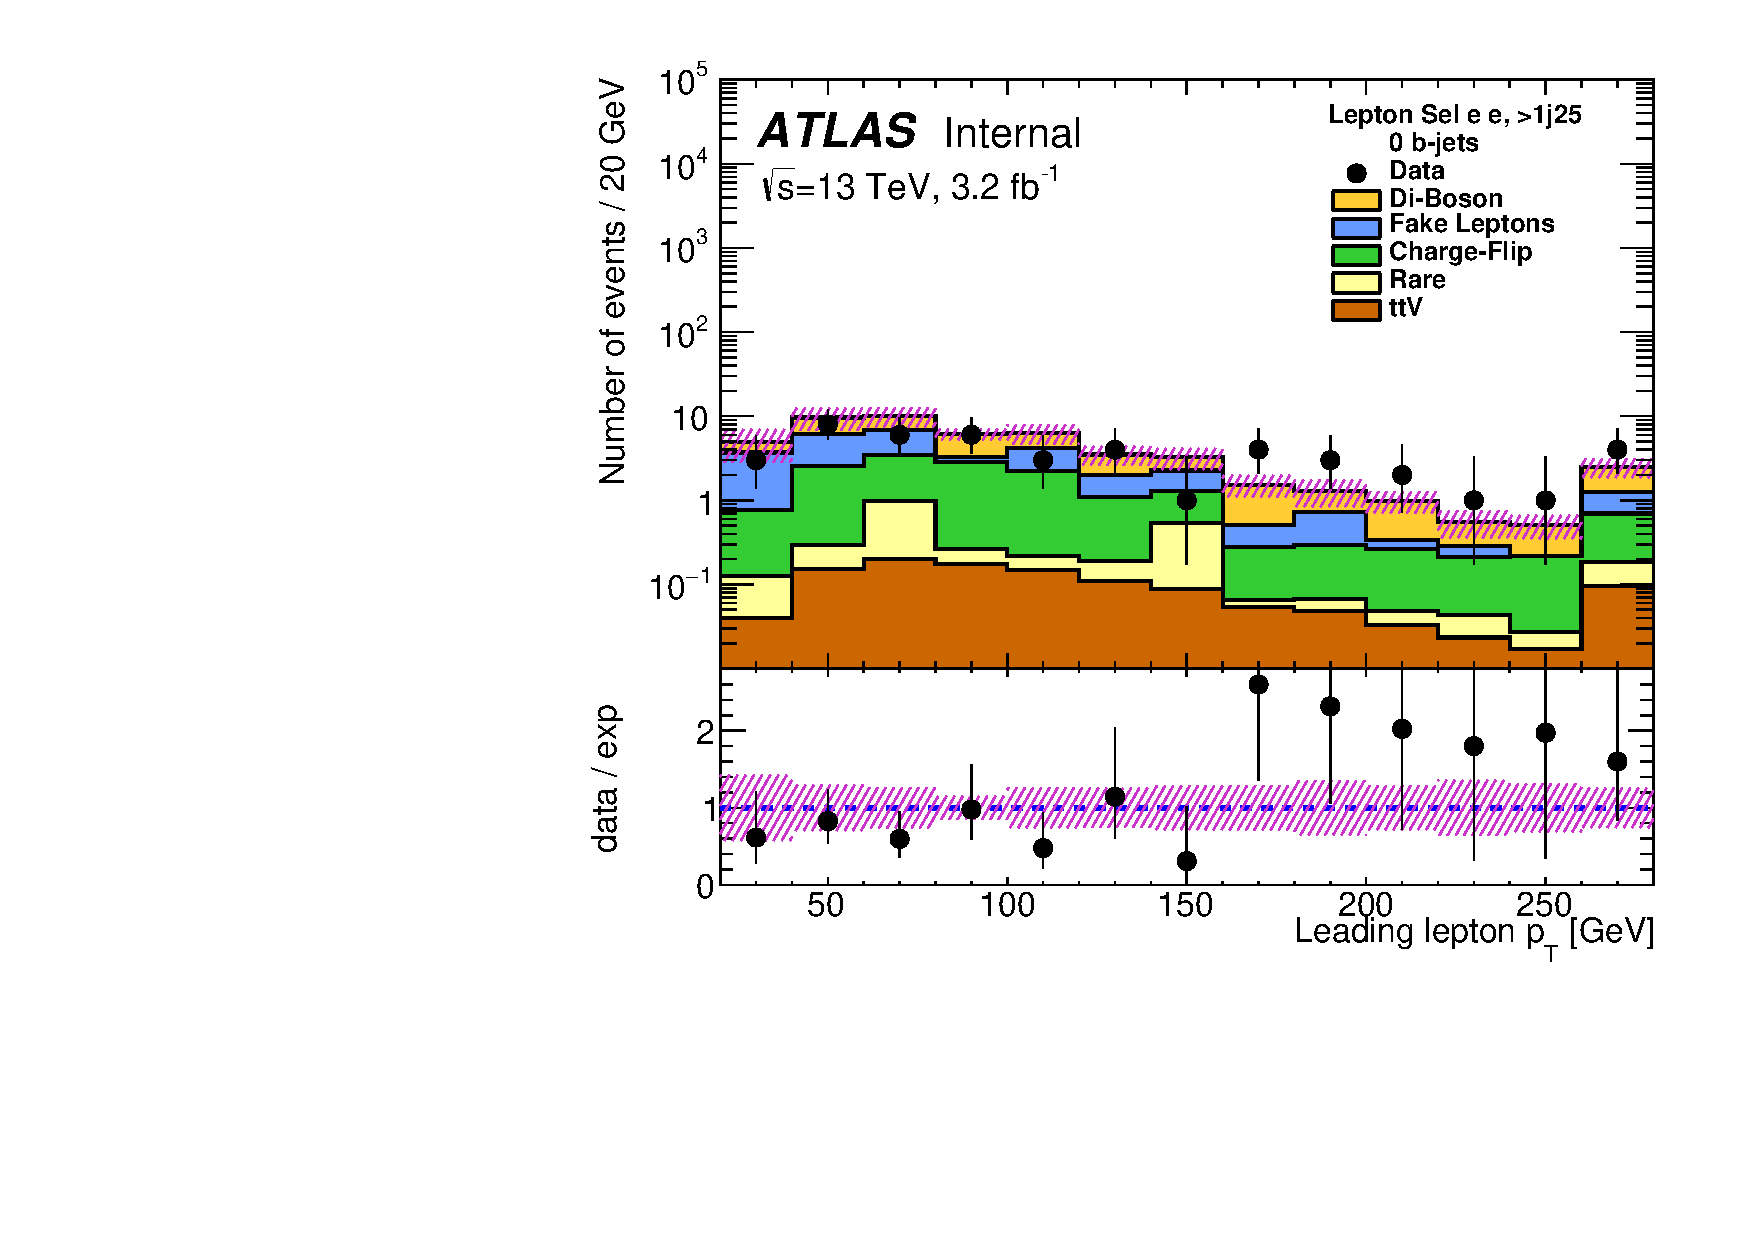
\includegraphics[width=0.5\textwidth]{BKG/validationPLots/PTLEP_EE_BVETOLEAD}
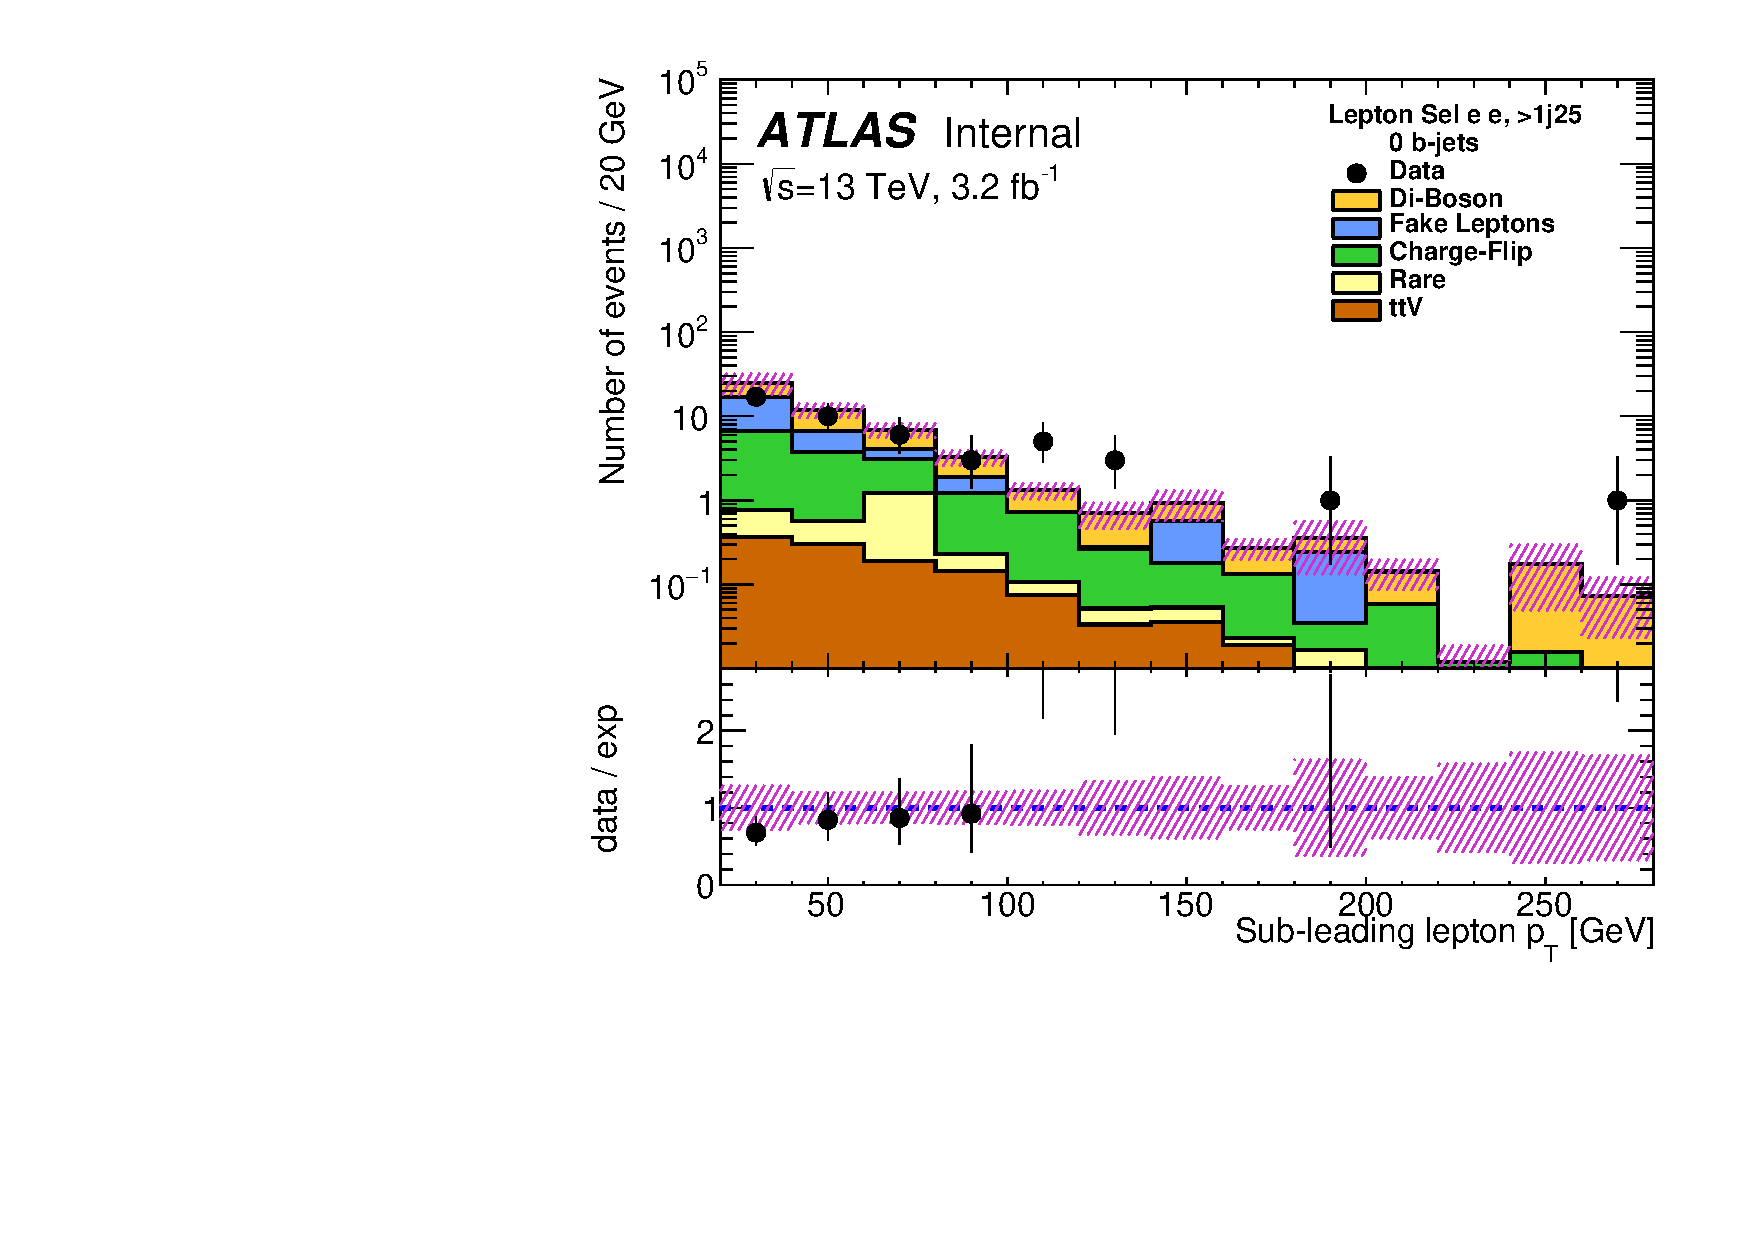
\includegraphics[width=0.5\textwidth]{BKG/validationPLots/PTLEP_EE_BVETOSUBLEAD}
}
\caption{$ee$ channel, \met $>$ 60\GeV and $N_{jets}^{25}$~$\ge$2: Distributions of \mt (top-left), selected leptons \pt (top-right), leading lepton \pt (bottom-left) and subleading lepton \pt (bottom-right) after lepton selections with with a $b$-jet veto (\pt~$>$~20~GeV).}
\label{Fig:VP_ee_0b_Njets_and_other}
\end{figure} 

\FloatBarrier


%%%%% emu channel, >= 1 b-jet
\begin{figure}[h!]
\centering
\subfigure{
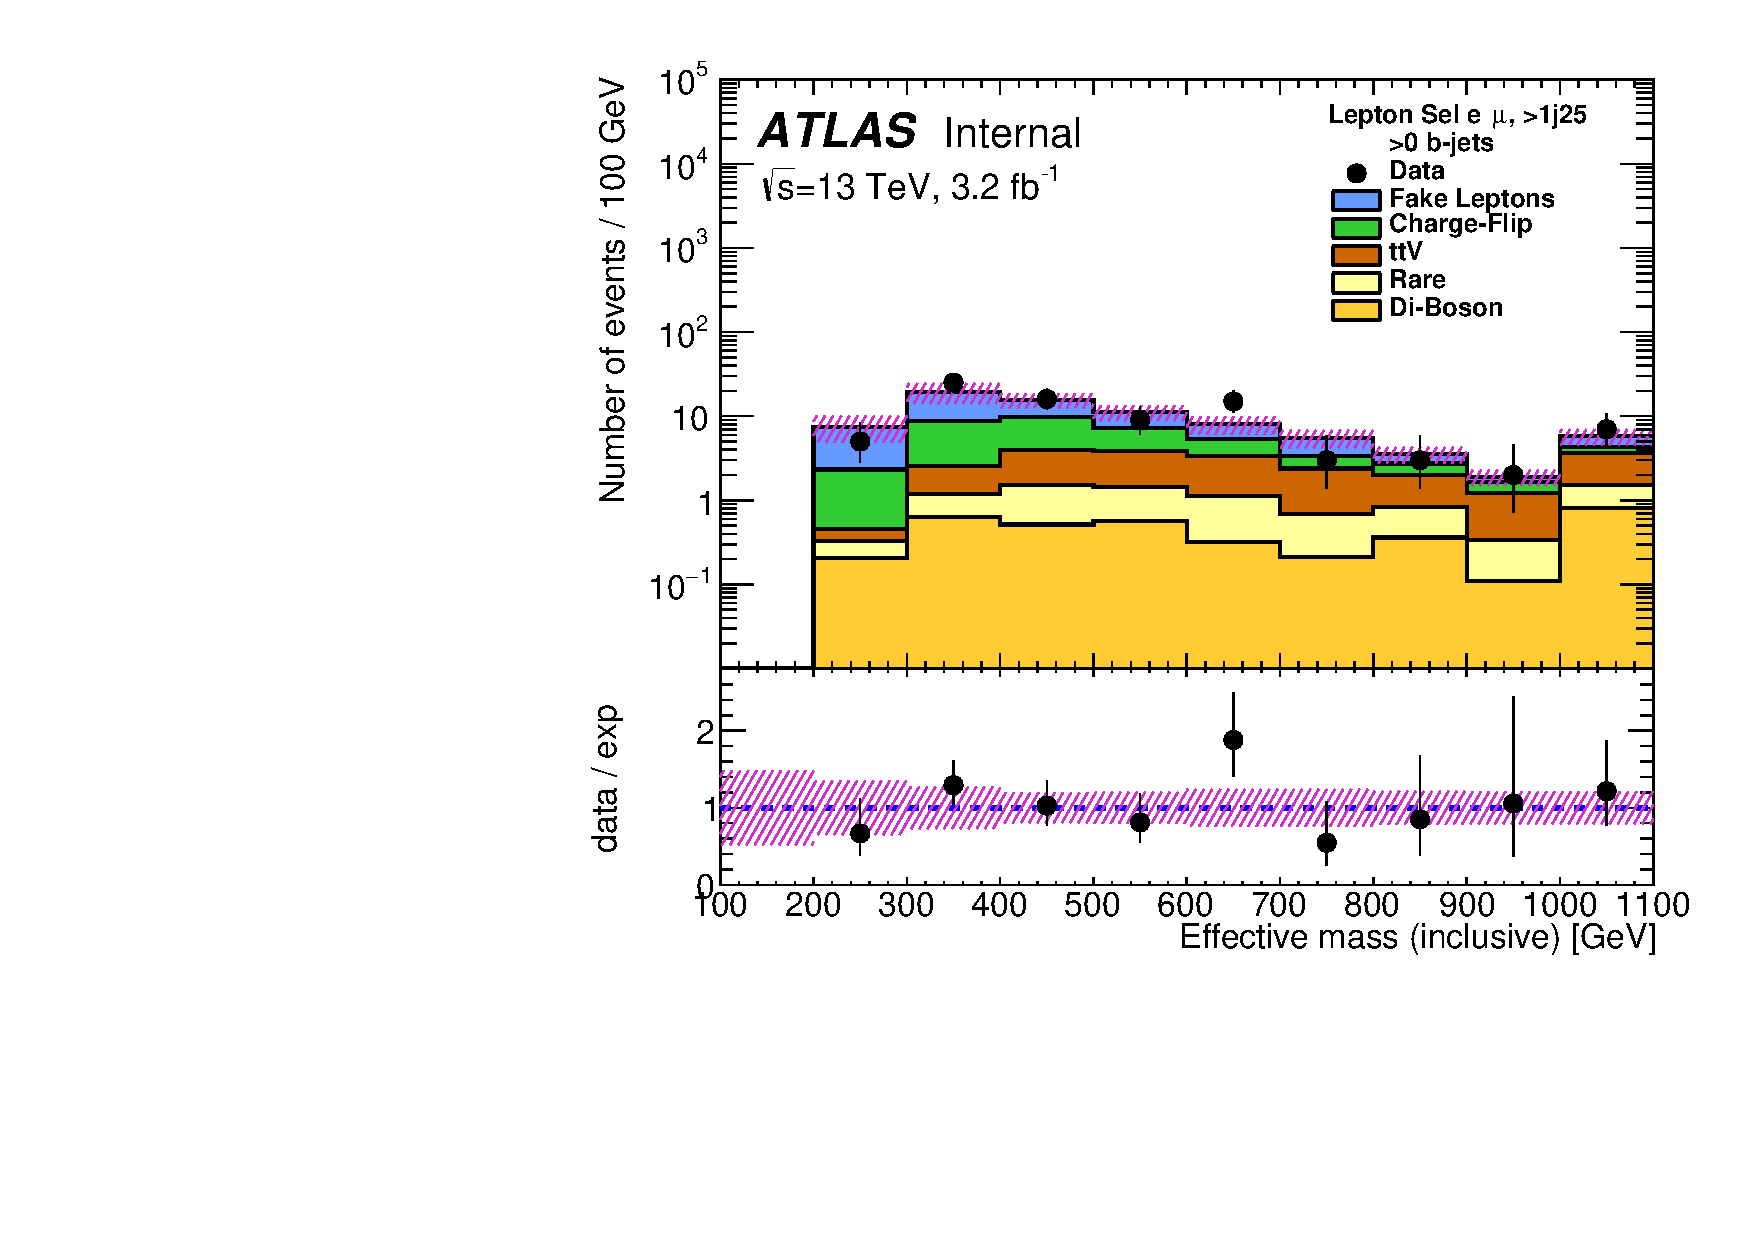
\includegraphics[width=0.5\textwidth]{BKG/validationPLots/MEFF_EM_LEP}
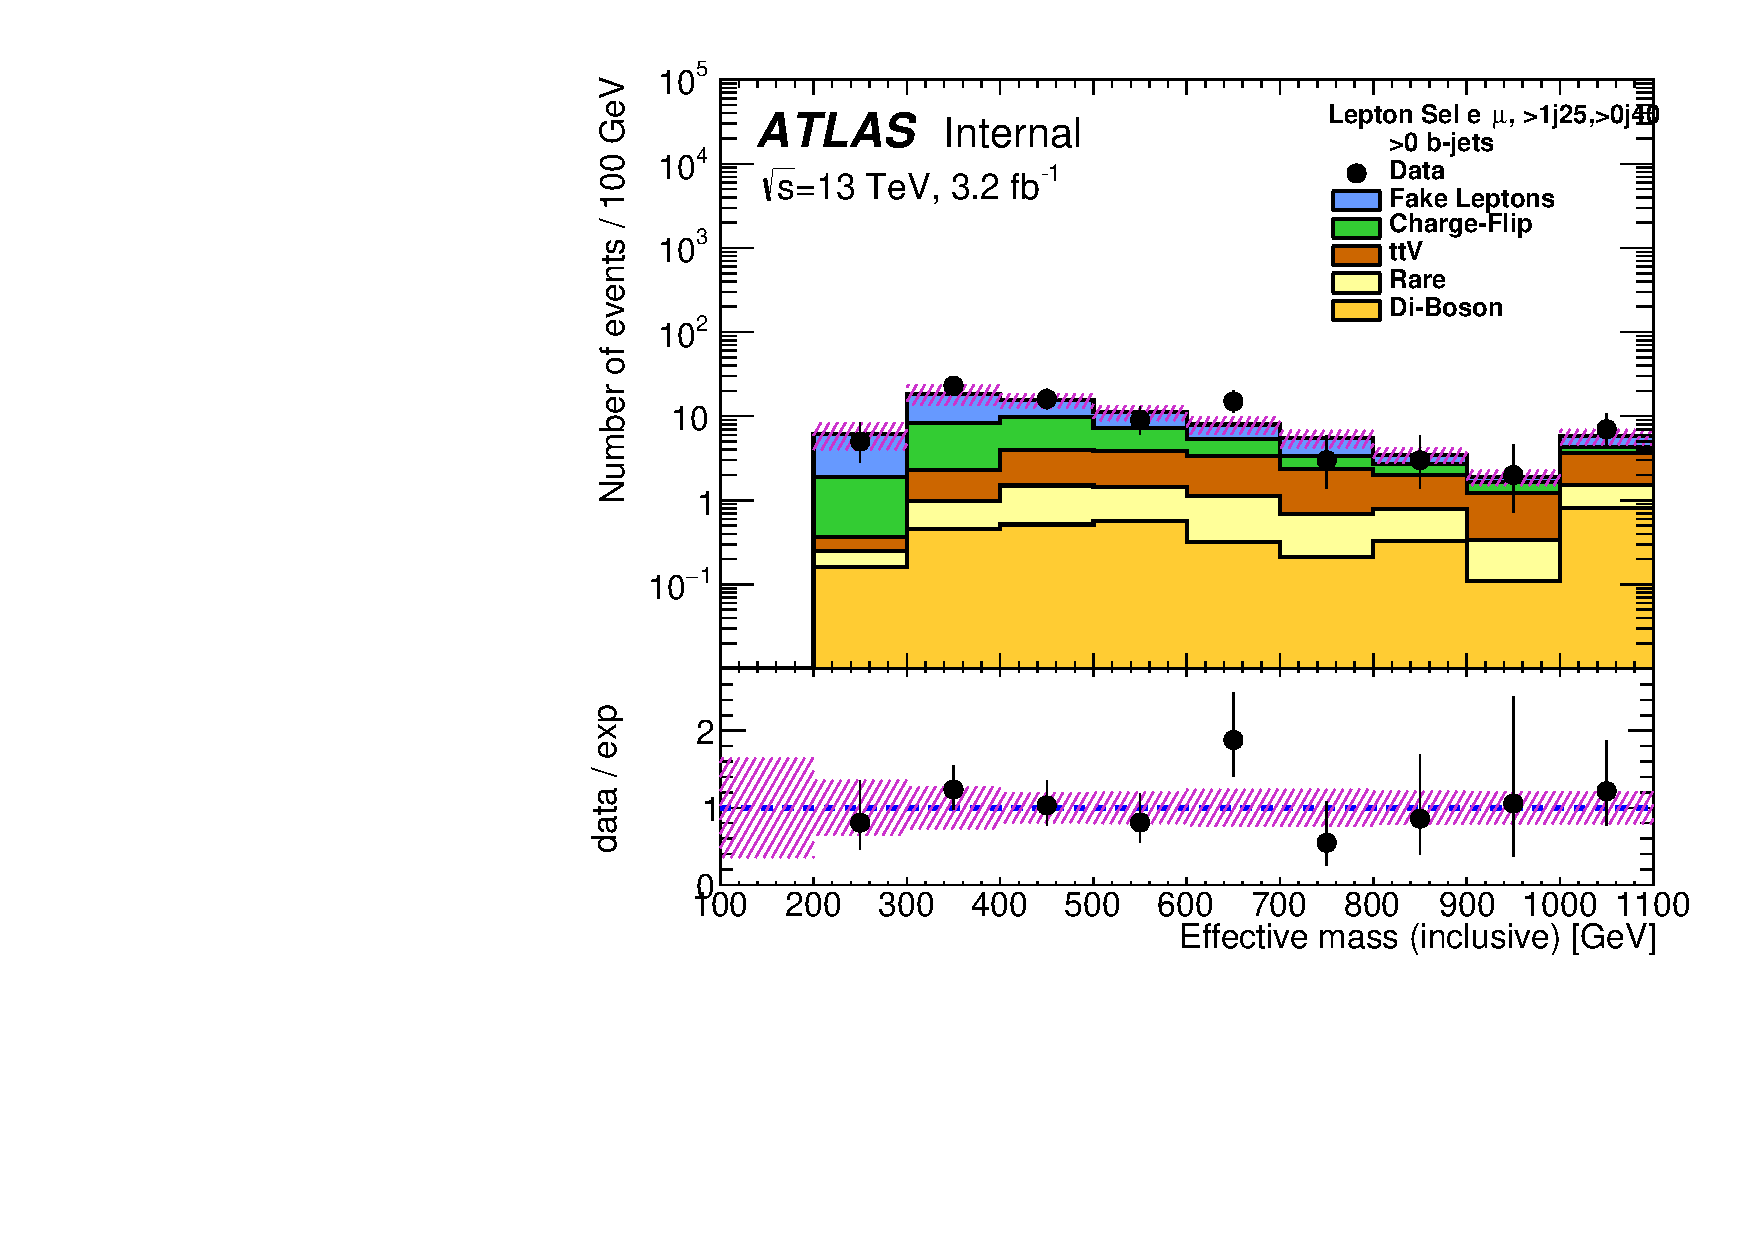
\includegraphics[width=0.5\textwidth]{BKG/validationPLots/MEFF_EM_L1JET}
}
\subfigure{
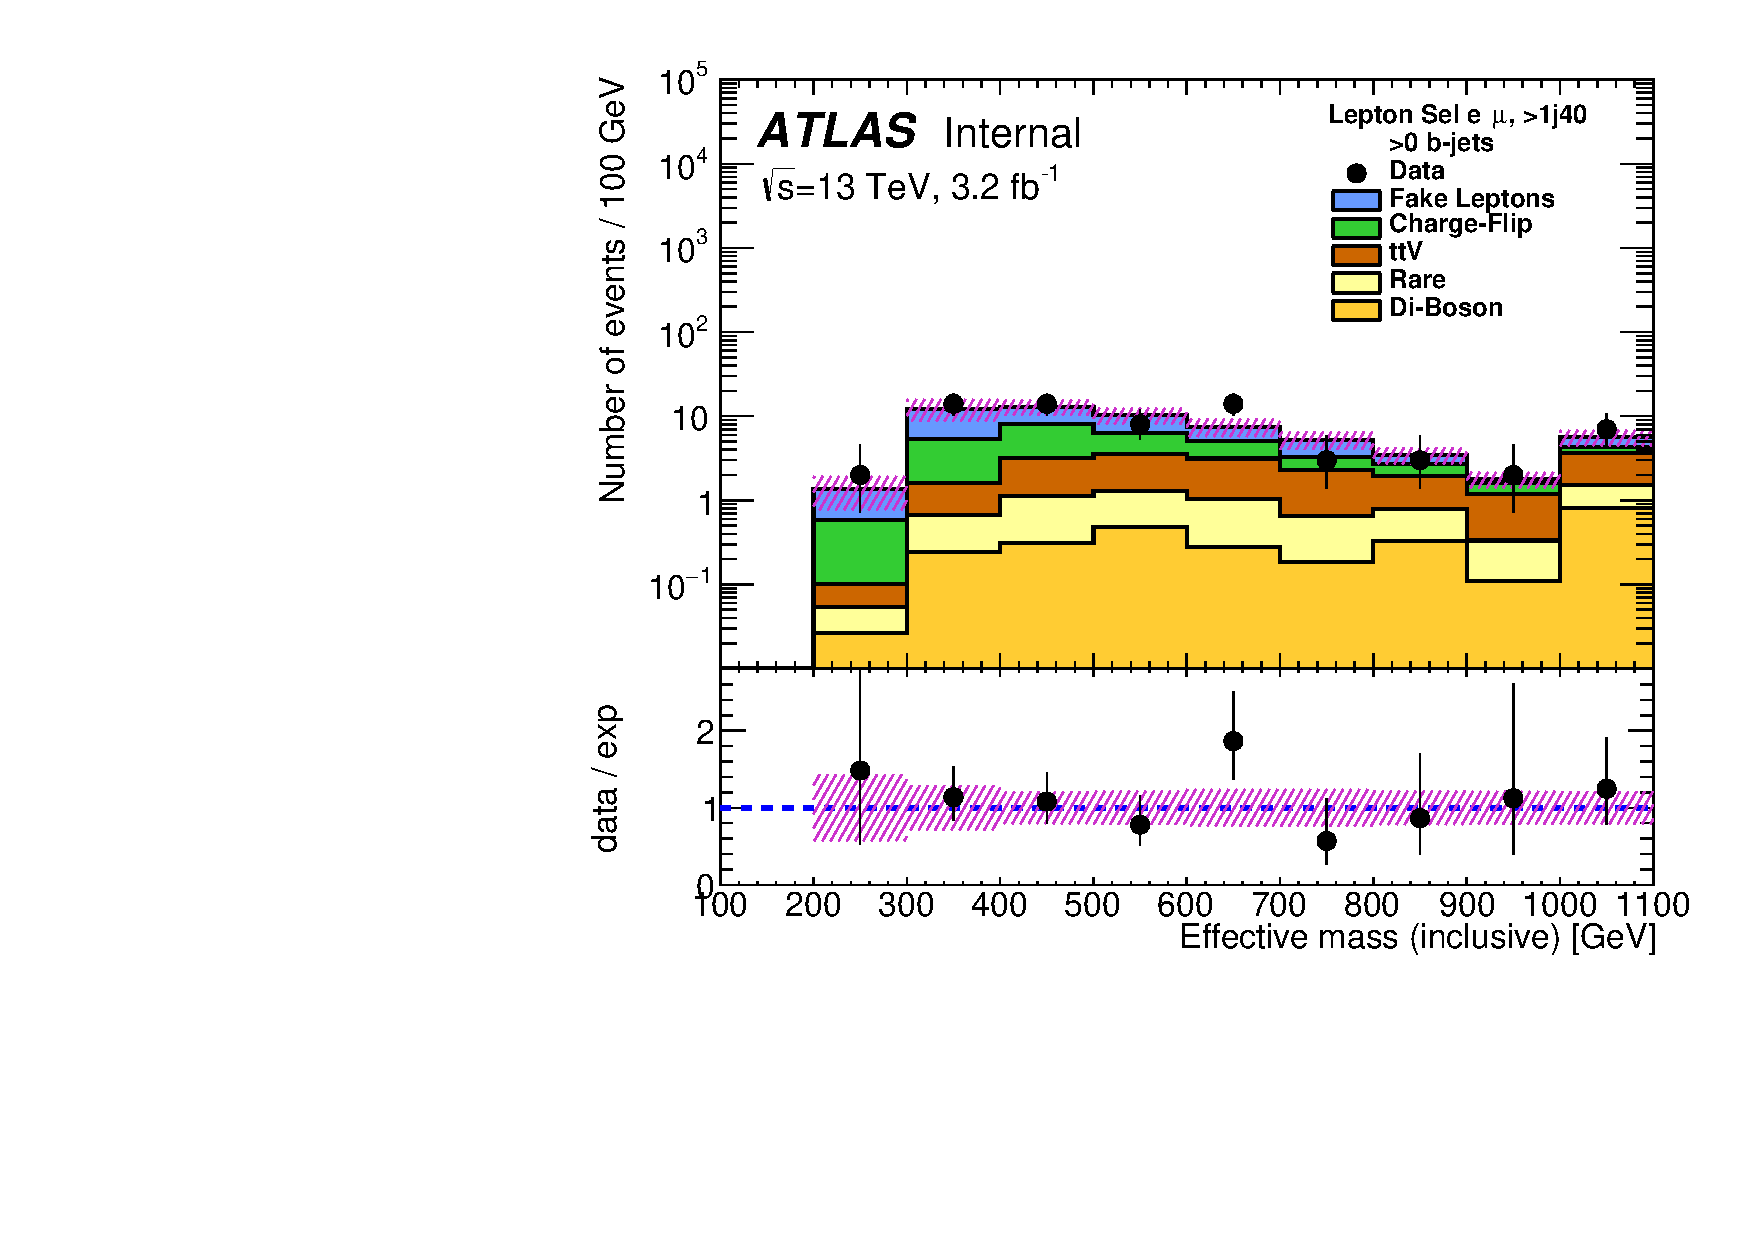
\includegraphics[width=0.5\textwidth]{BKG/validationPLots/MEFF_EM_L2JET}
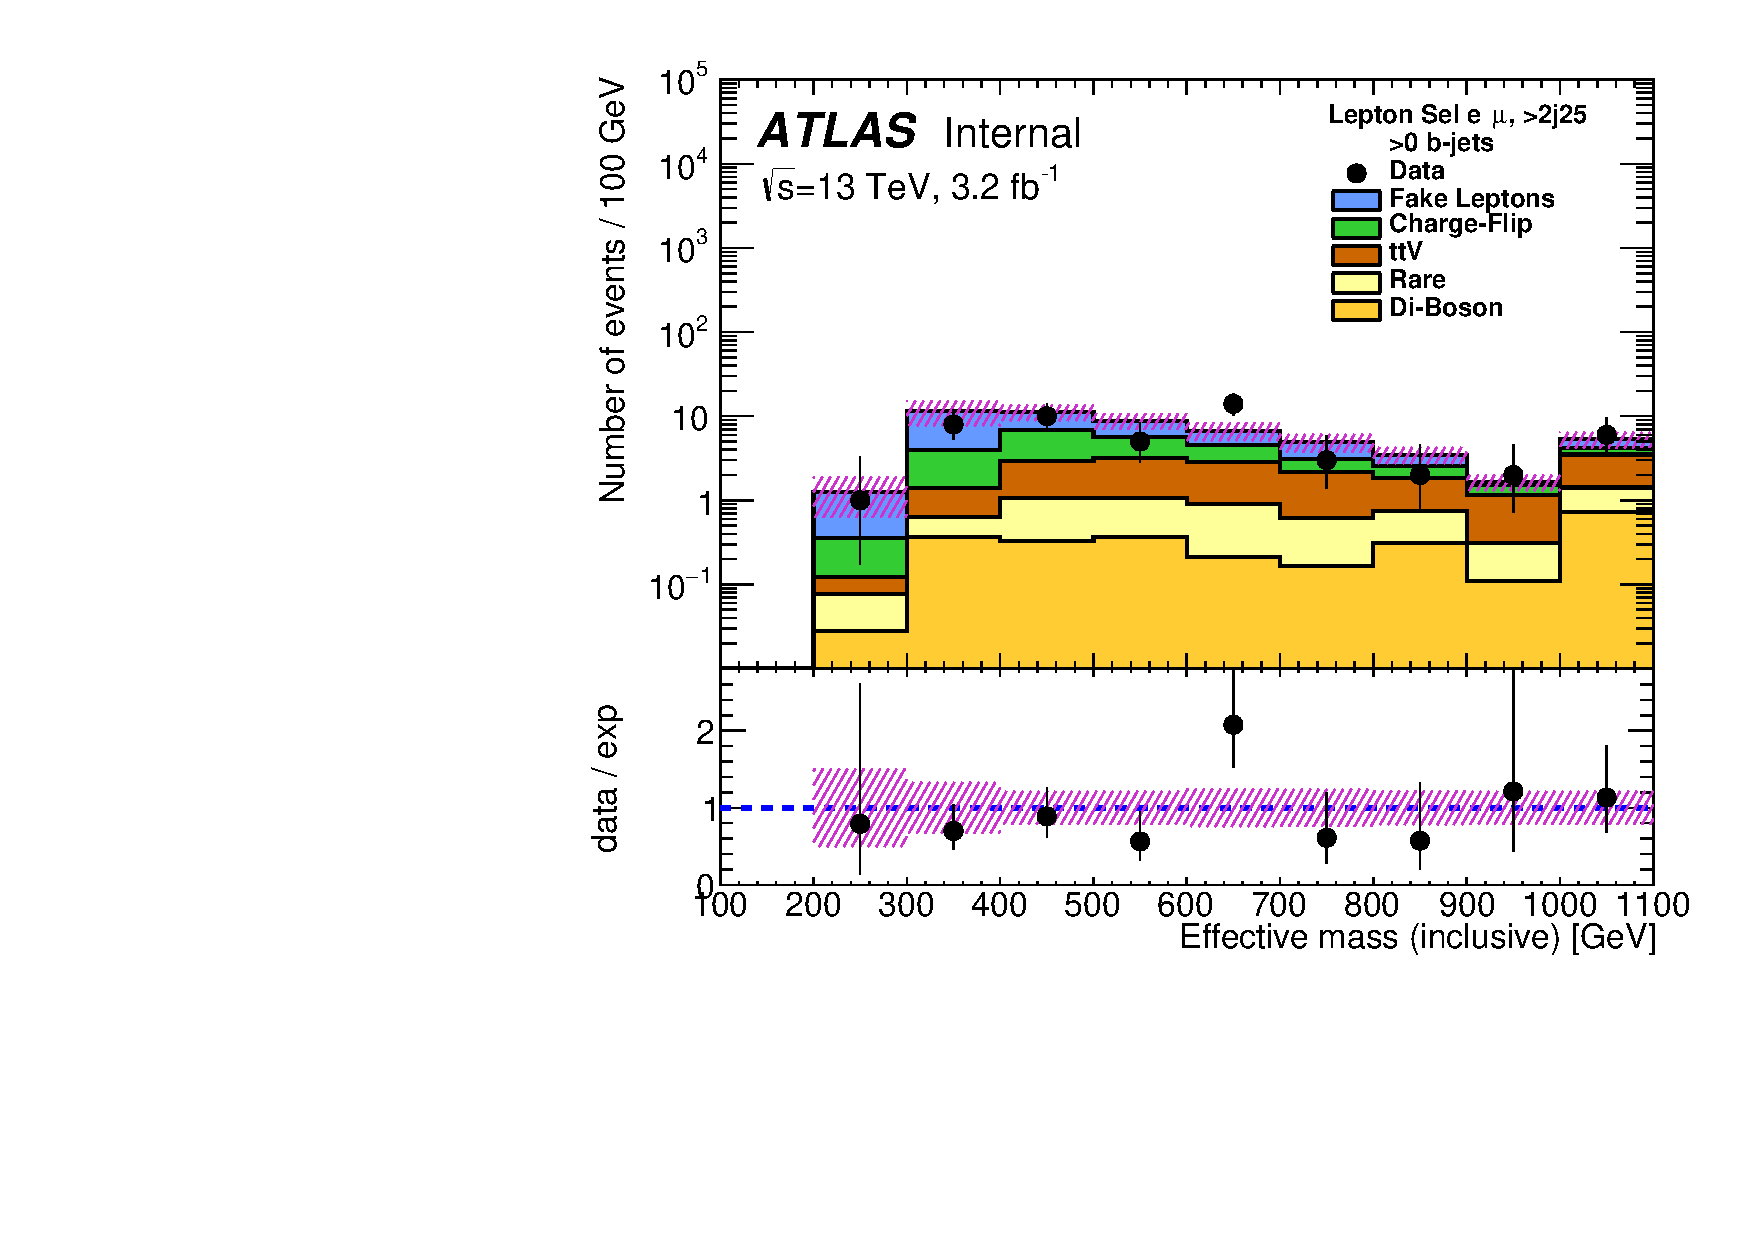
\includegraphics[width=0.5\textwidth]{BKG/validationPLots/MEFF_EM_L3JET}
}
\caption{$e\mu$ channel, \met $>$ 60\GeV and $N_{jets}^{25}$~$\ge$2: Effective mass distribution after lepton selections with at least one $b$-jet (\pt~$>$~20~GeV) and with at least 0, 1, 2 and 3 jets with \pt~$>$~40~GeV (from top-left to bottom-right).}
\label{Fig:VP_em_1b_Meff}
\end{figure}
%%
\begin{figure}[h!]
\centering
\subfigure{
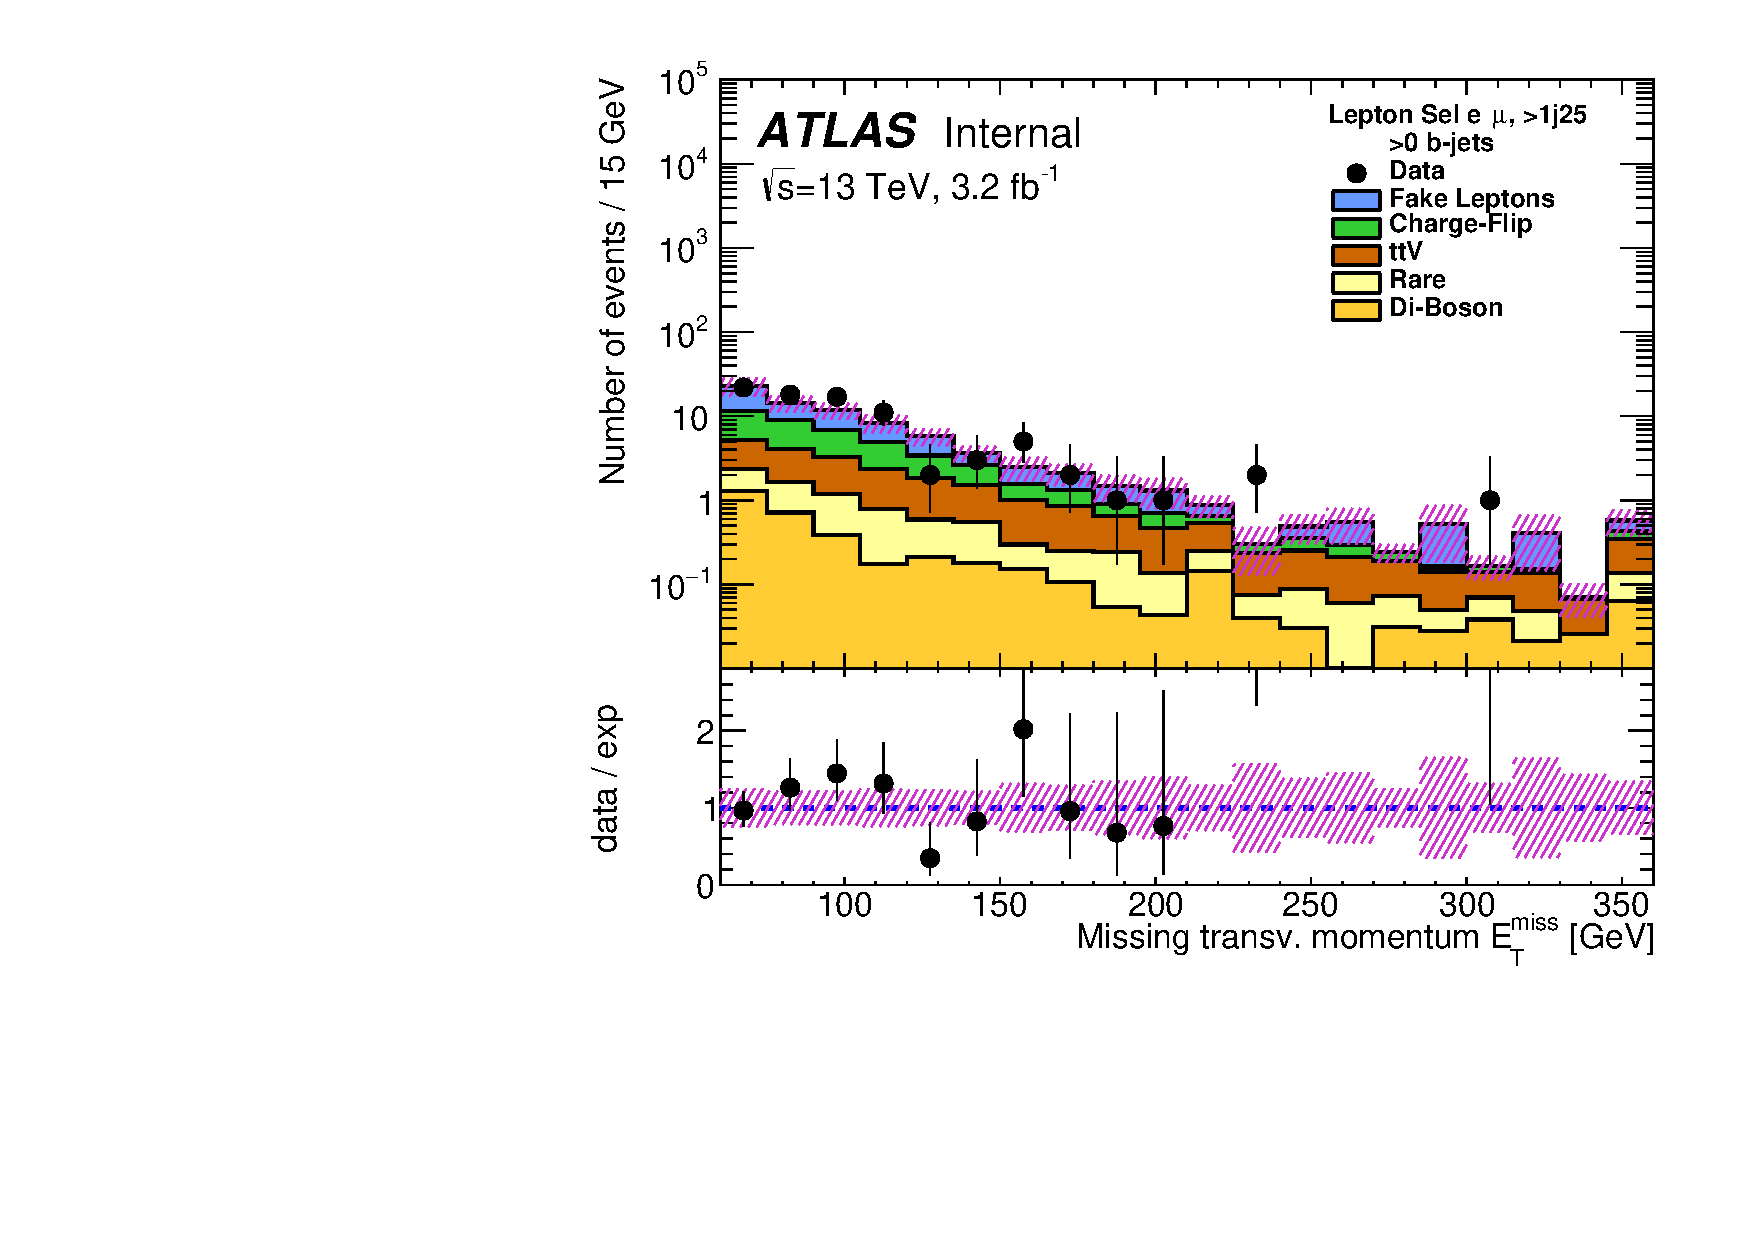
\includegraphics[width=0.5\textwidth]{BKG/validationPLots/MET_EM_LEP}
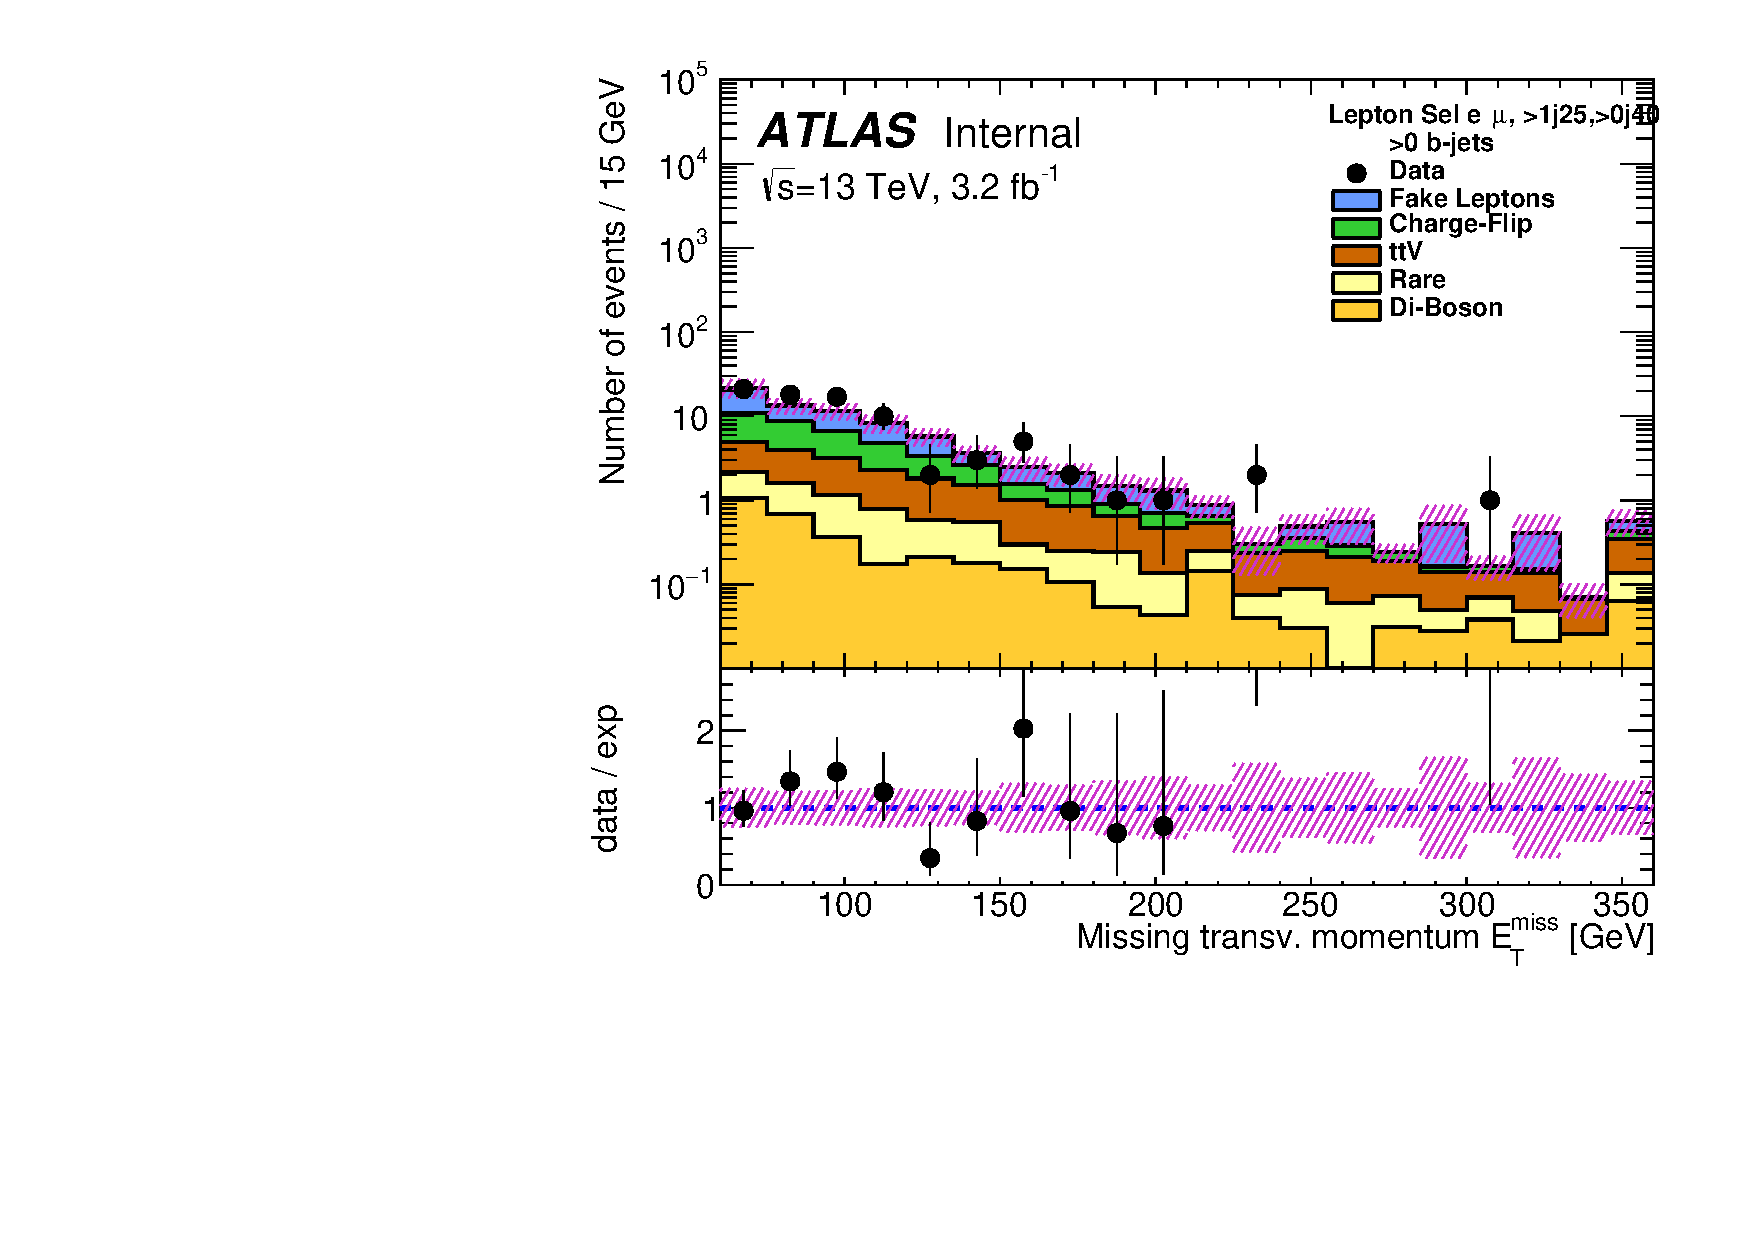
\includegraphics[width=0.5\textwidth]{BKG/validationPLots/MET_EM_L1JET}
}
\subfigure{
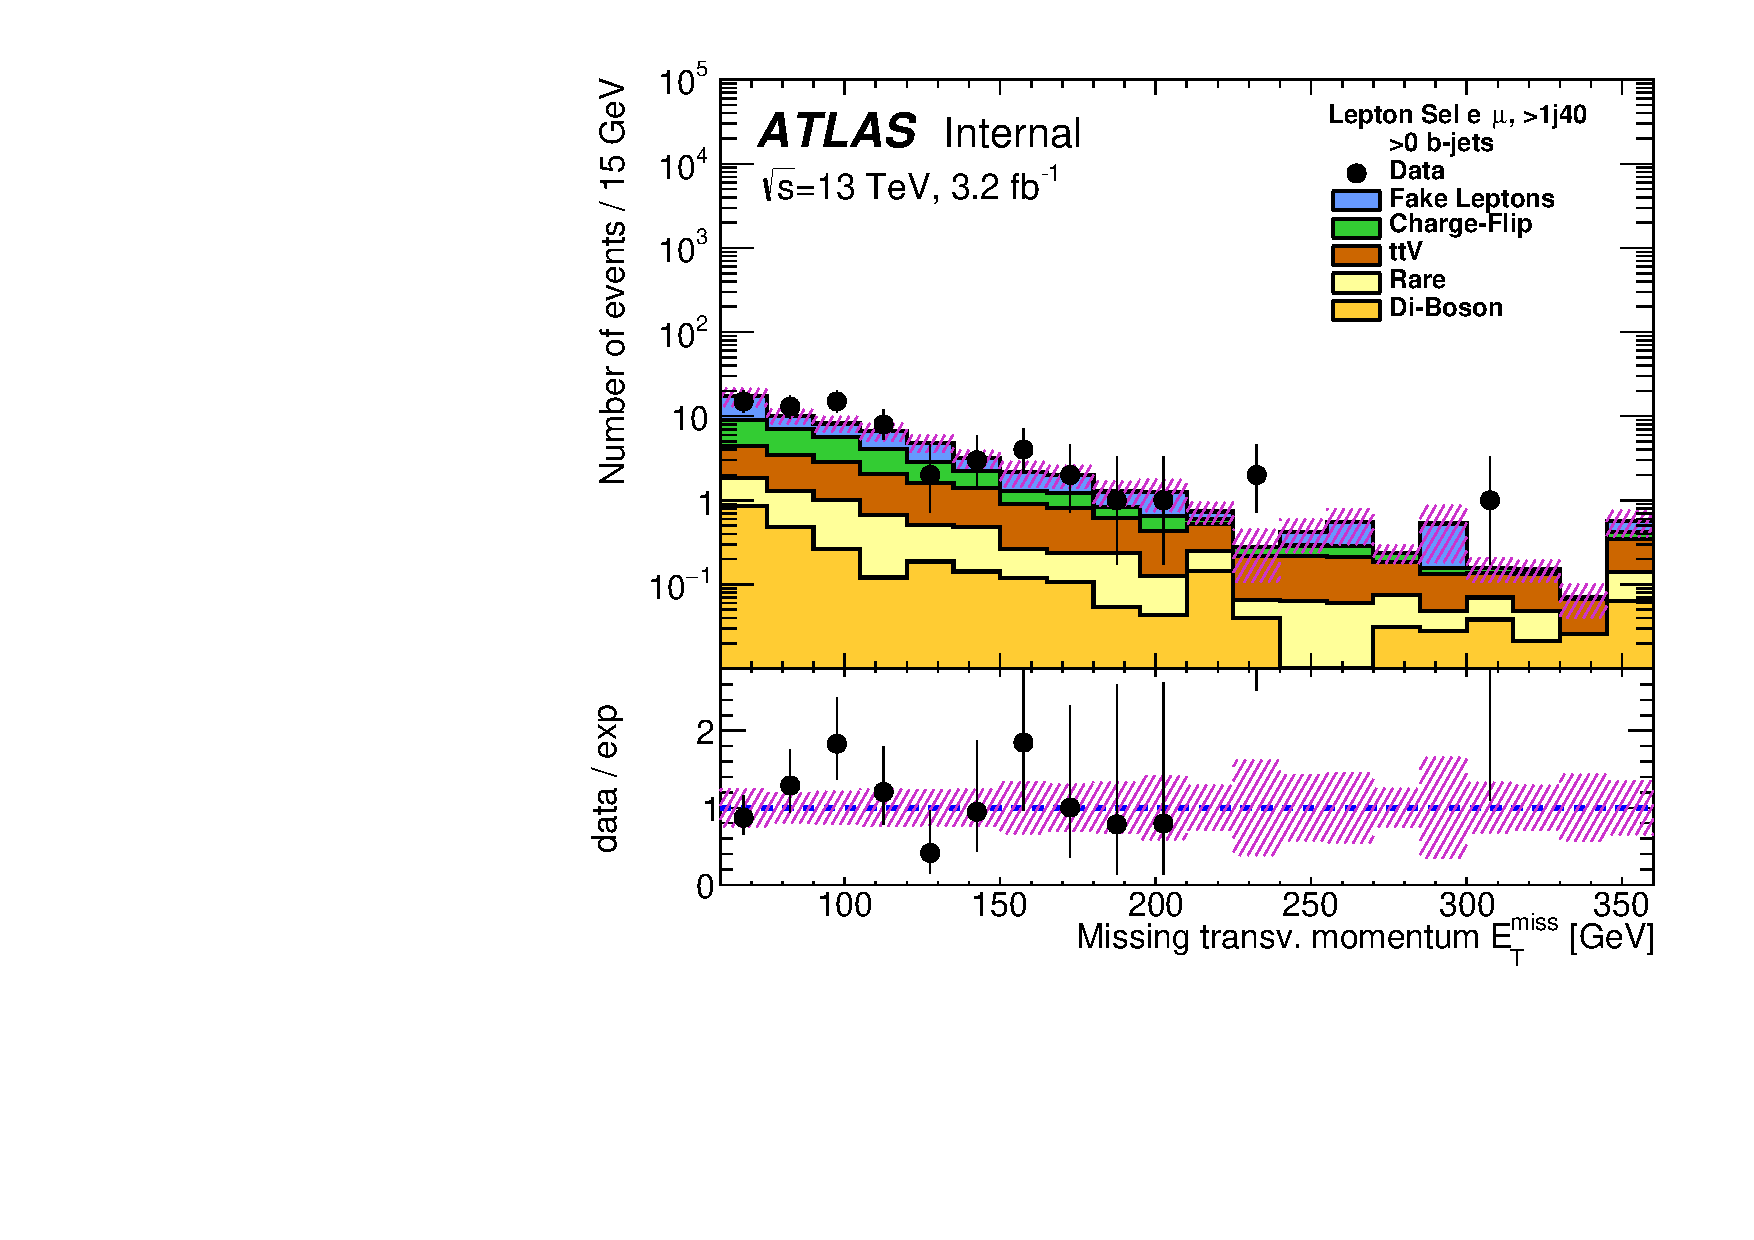
\includegraphics[width=0.5\textwidth]{BKG/validationPLots/MET_EM_L2JET}
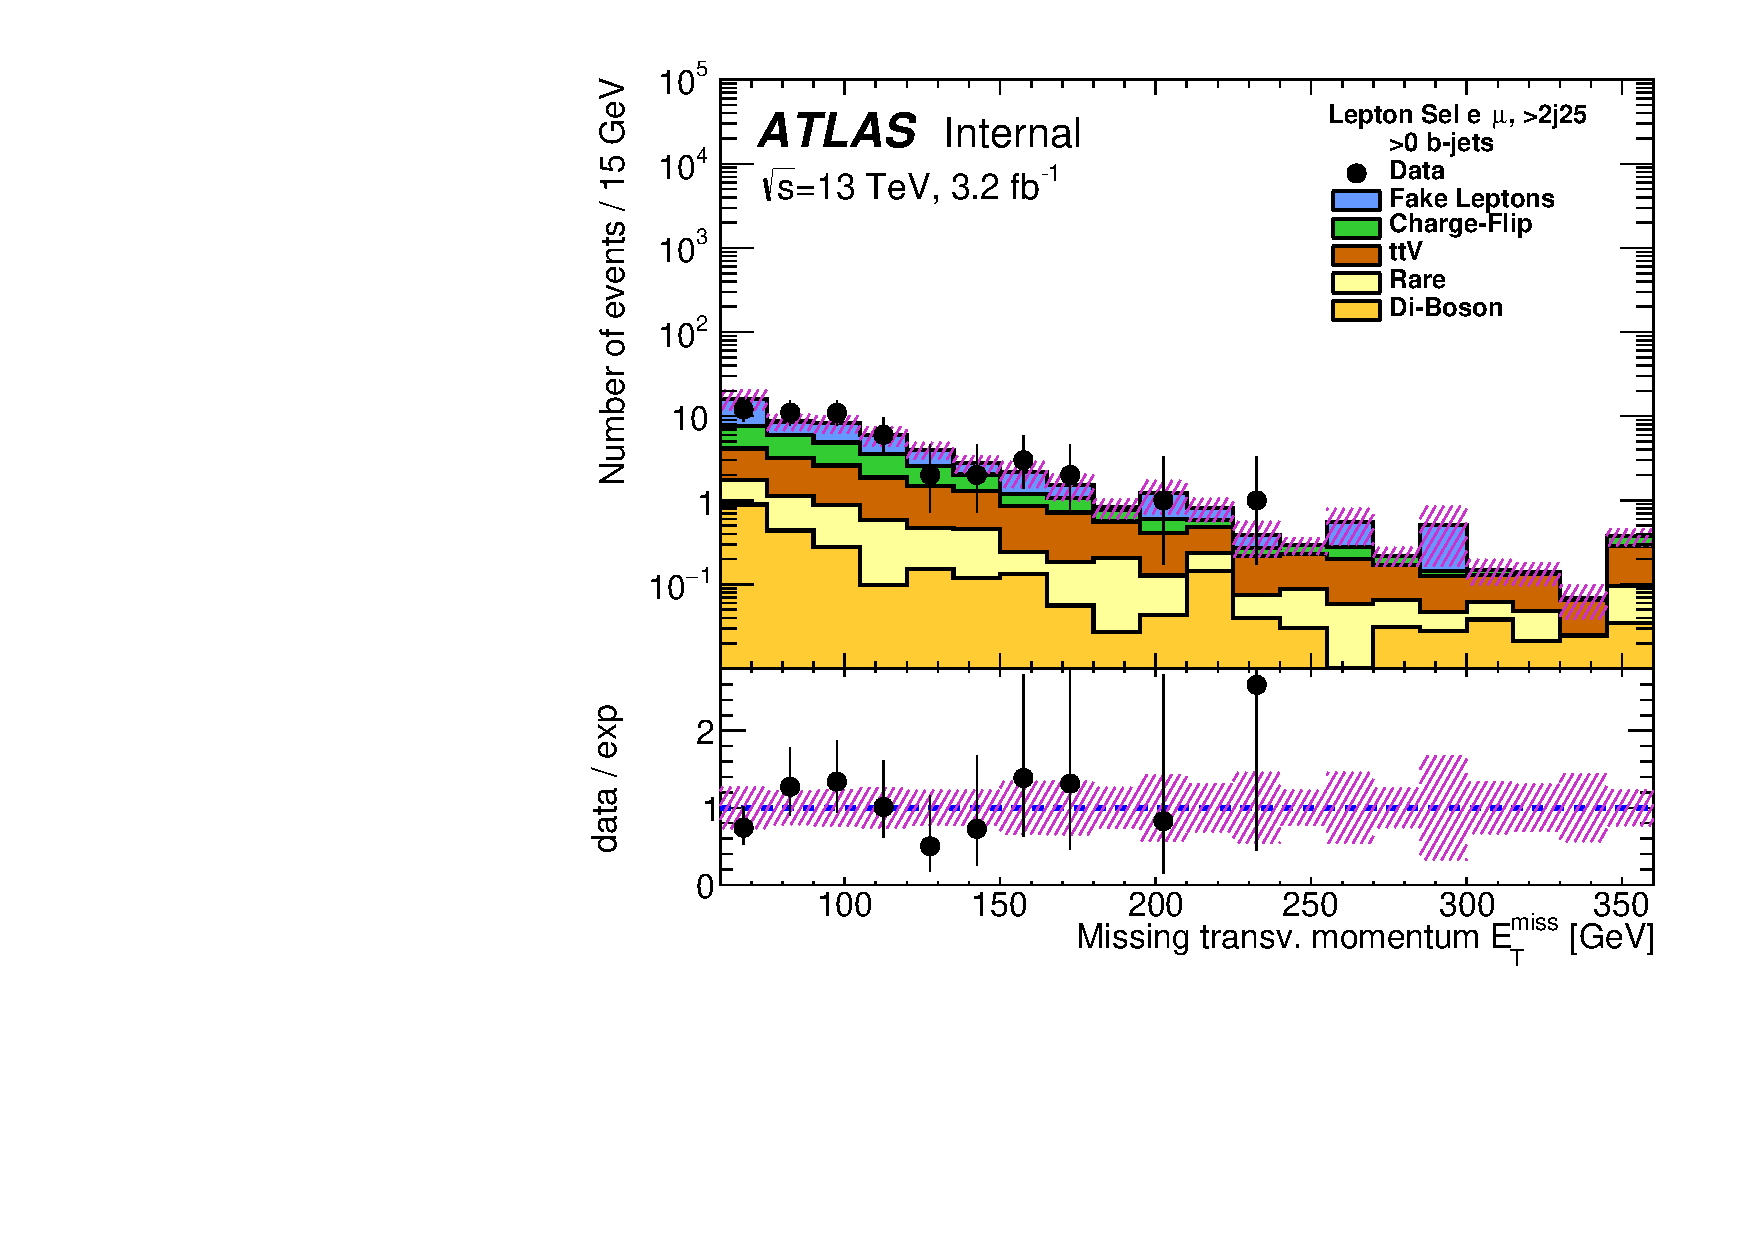
\includegraphics[width=0.5\textwidth]{BKG/validationPLots/MET_EM_L3JET}
}
\caption{$e\mu$ channel, \met $>$ 60\GeV and $N_{jets}^{25}$~$\ge$2: Missing transverse energy distribution after lepton selections with at least one $b$-jet (\pt~$>$~20~GeV) and with at least 0, 1, 2 and 3 jets with \pt~$>$~40~GeV (from top-left to bottom-right).}
\label{Fig:VP_em_1b_Met}
\end{figure}
%%
\begin{figure}[h!]
\centering
\subfigure{
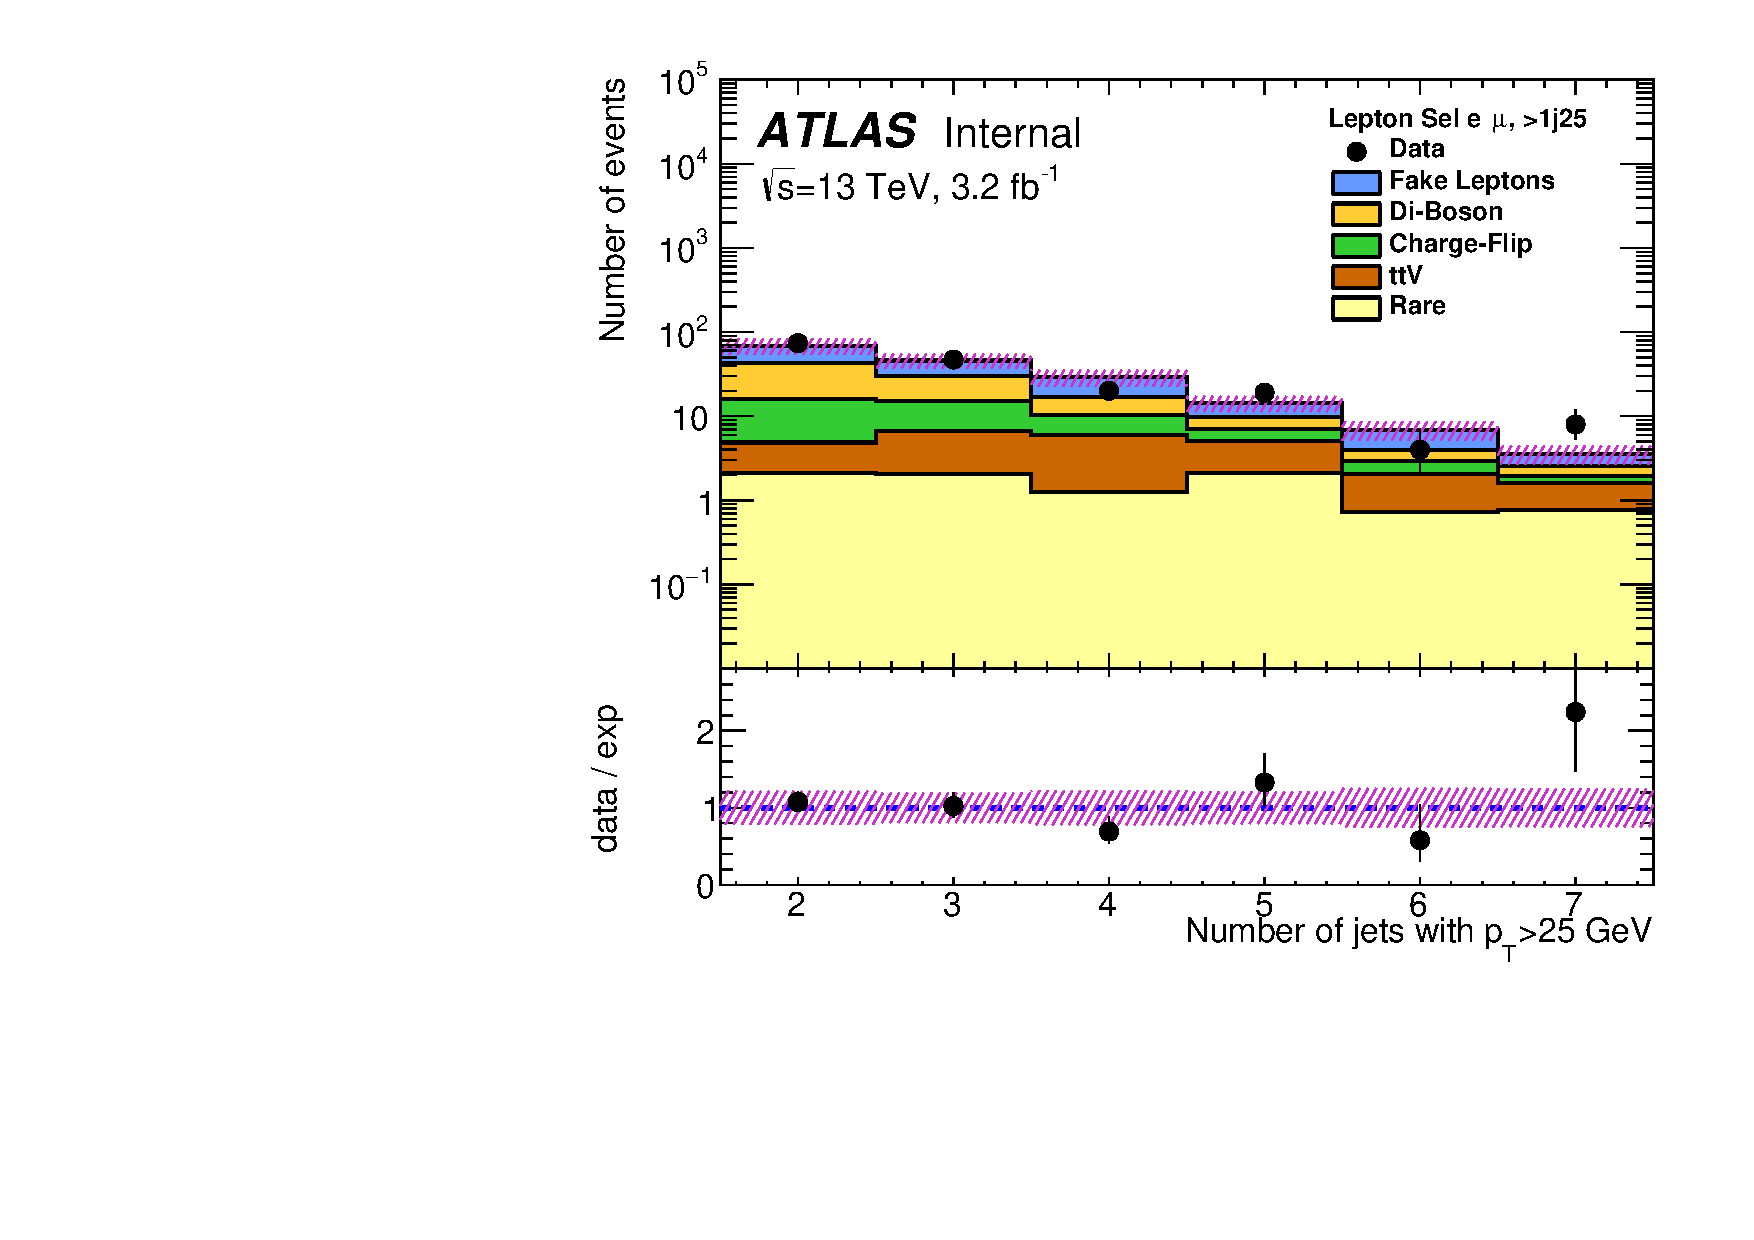
\includegraphics[width=0.45\textwidth]{BKG/validationPLots/NJETS40_EM_LEP}
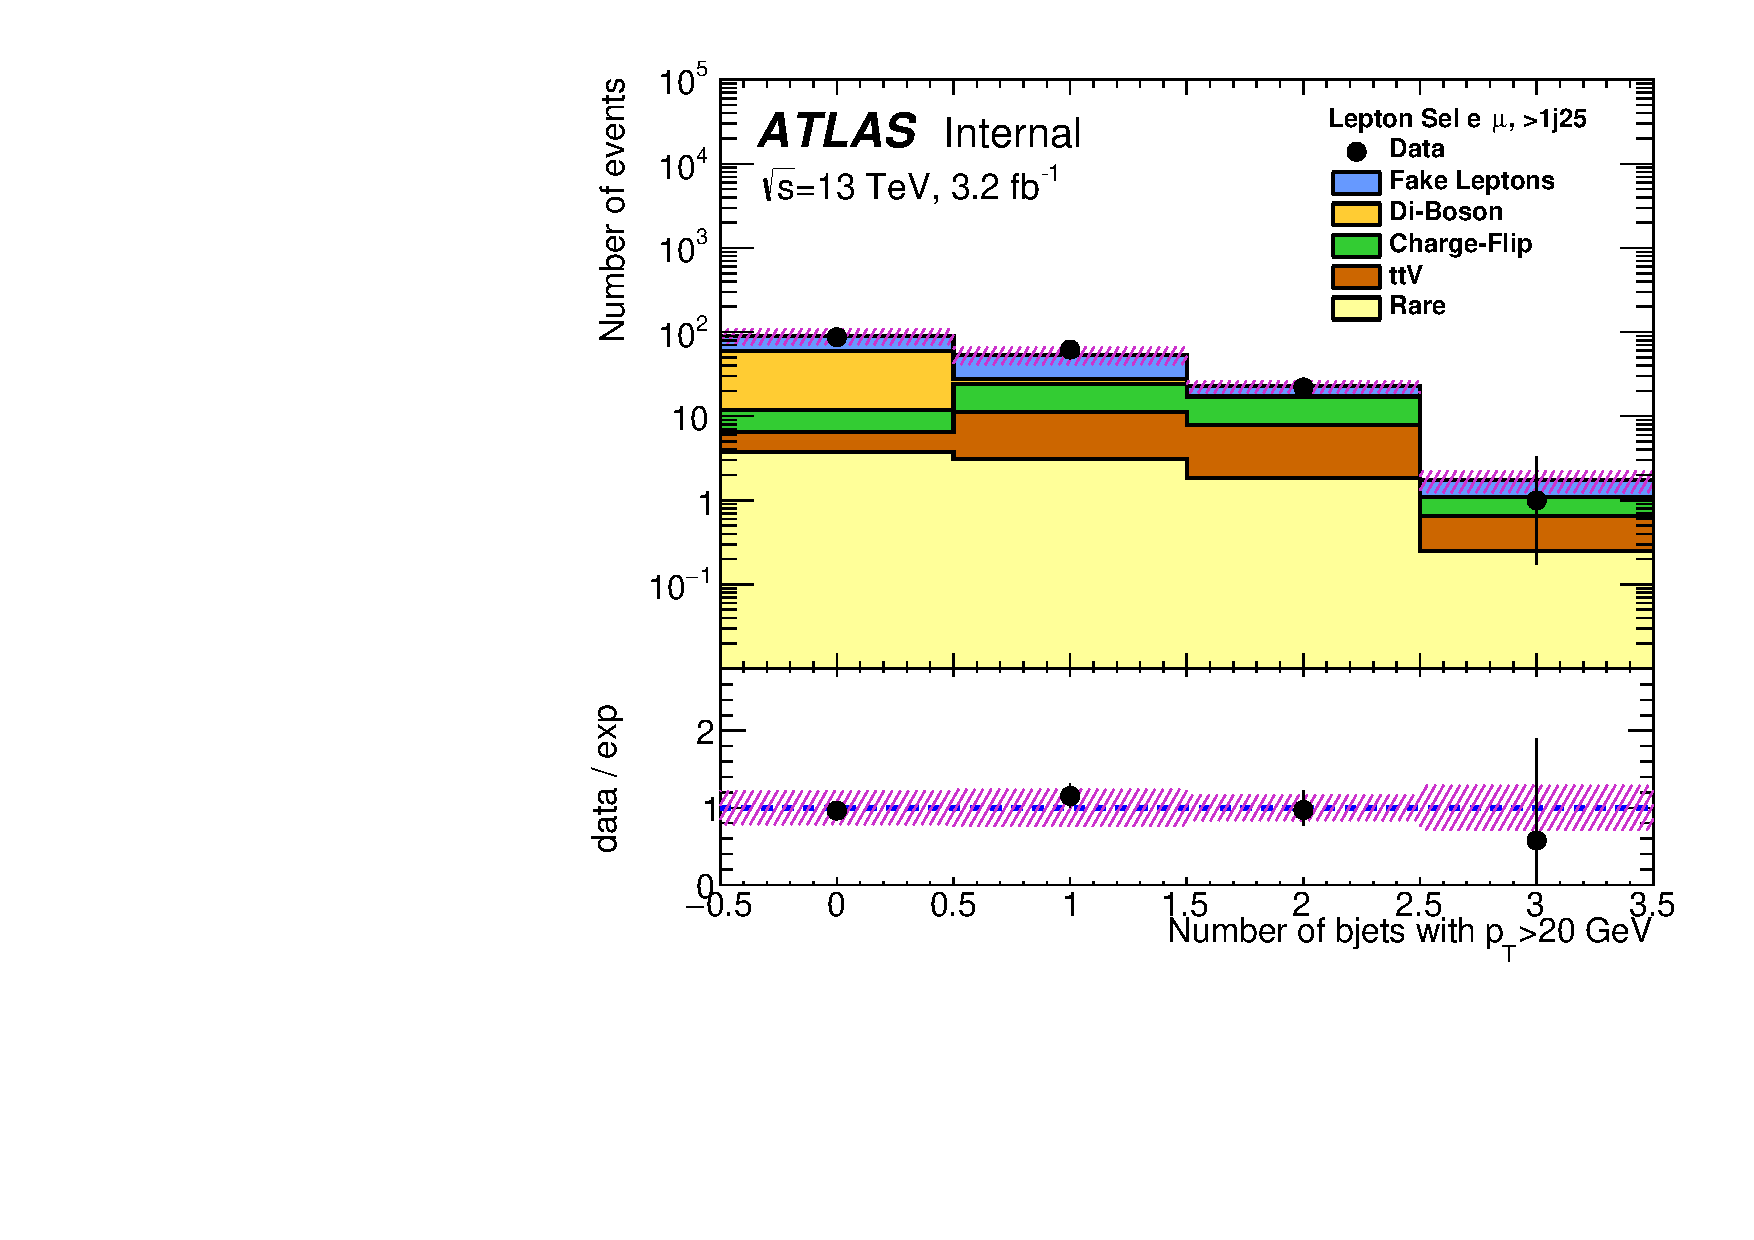
\includegraphics[width=0.45\textwidth]{BKG/validationPLots/NBJETS20_EM_LEP}
}
\subfigure{
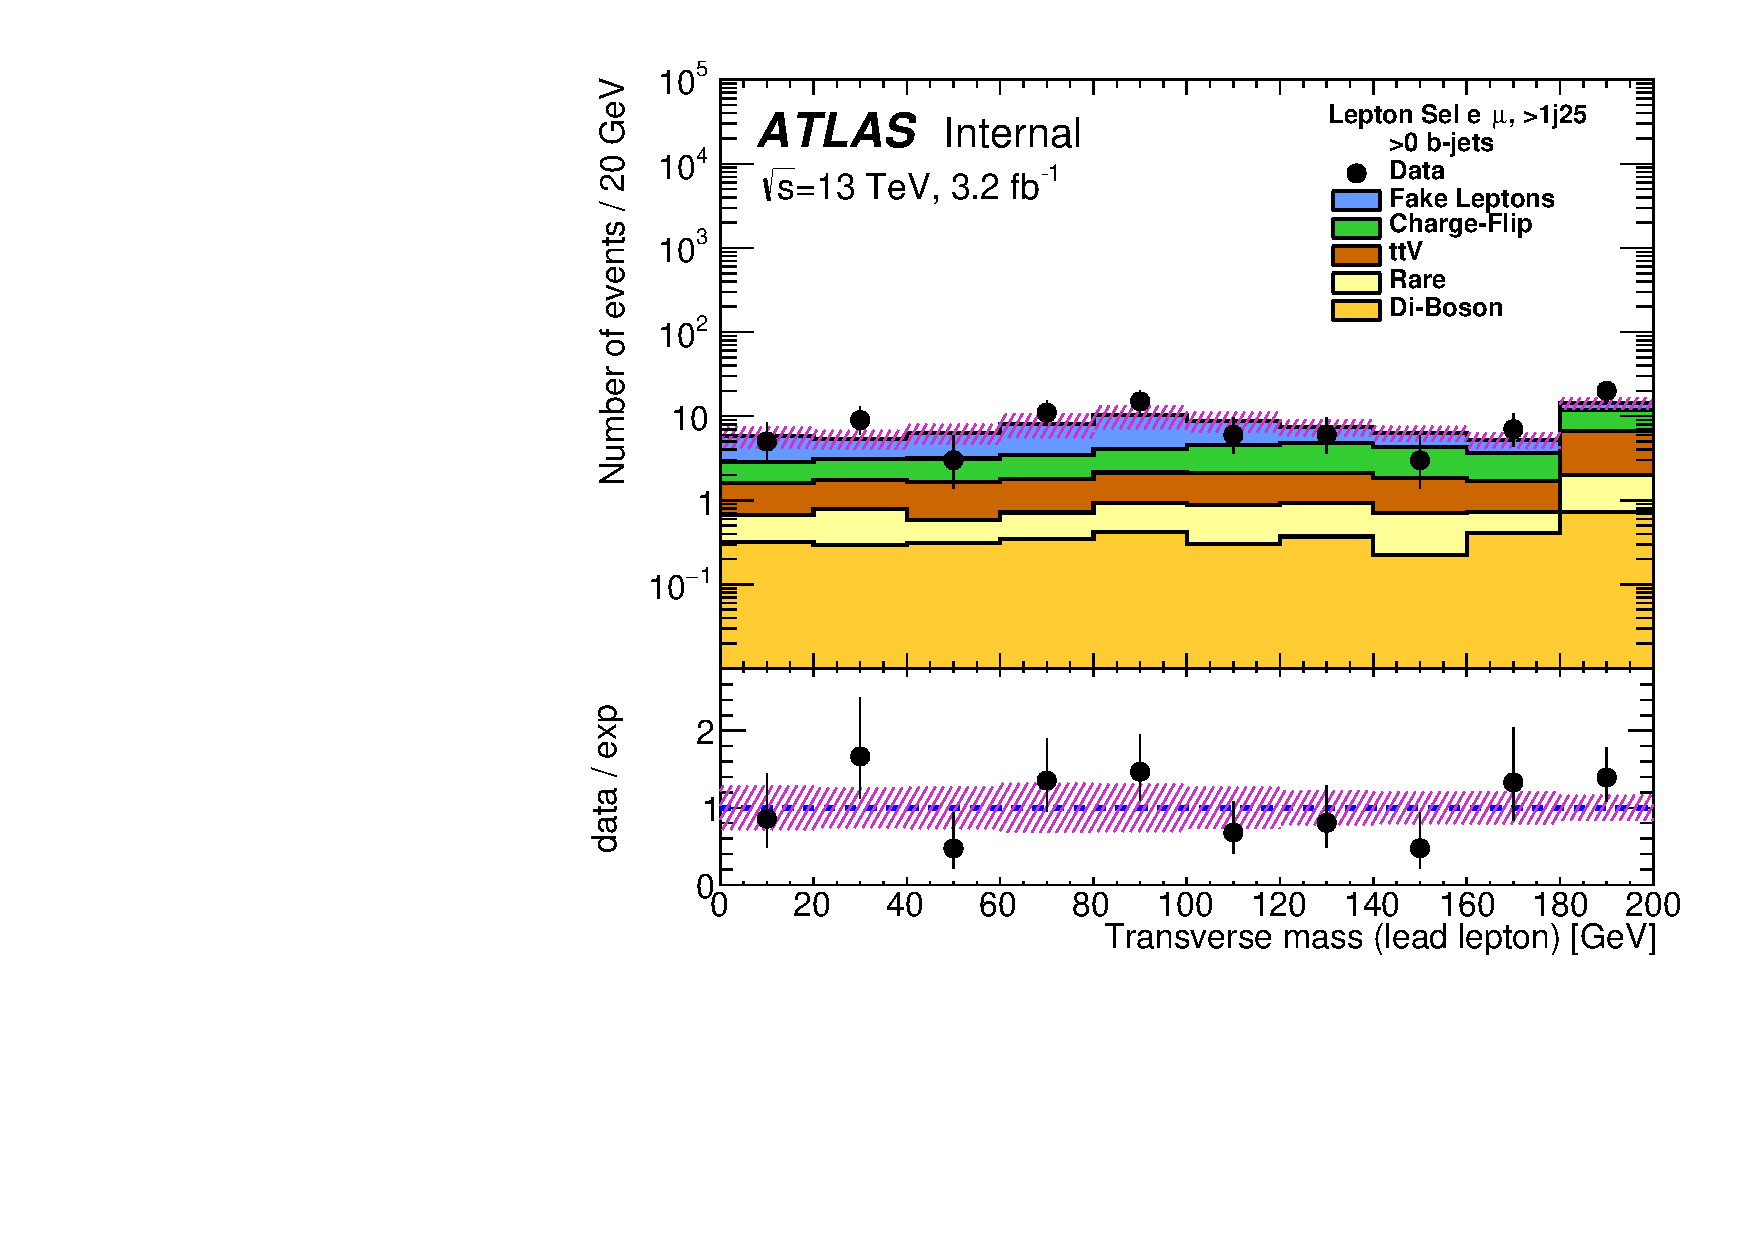
\includegraphics[width=0.45\textwidth]{BKG/validationPLots/MT_EM_LEP}
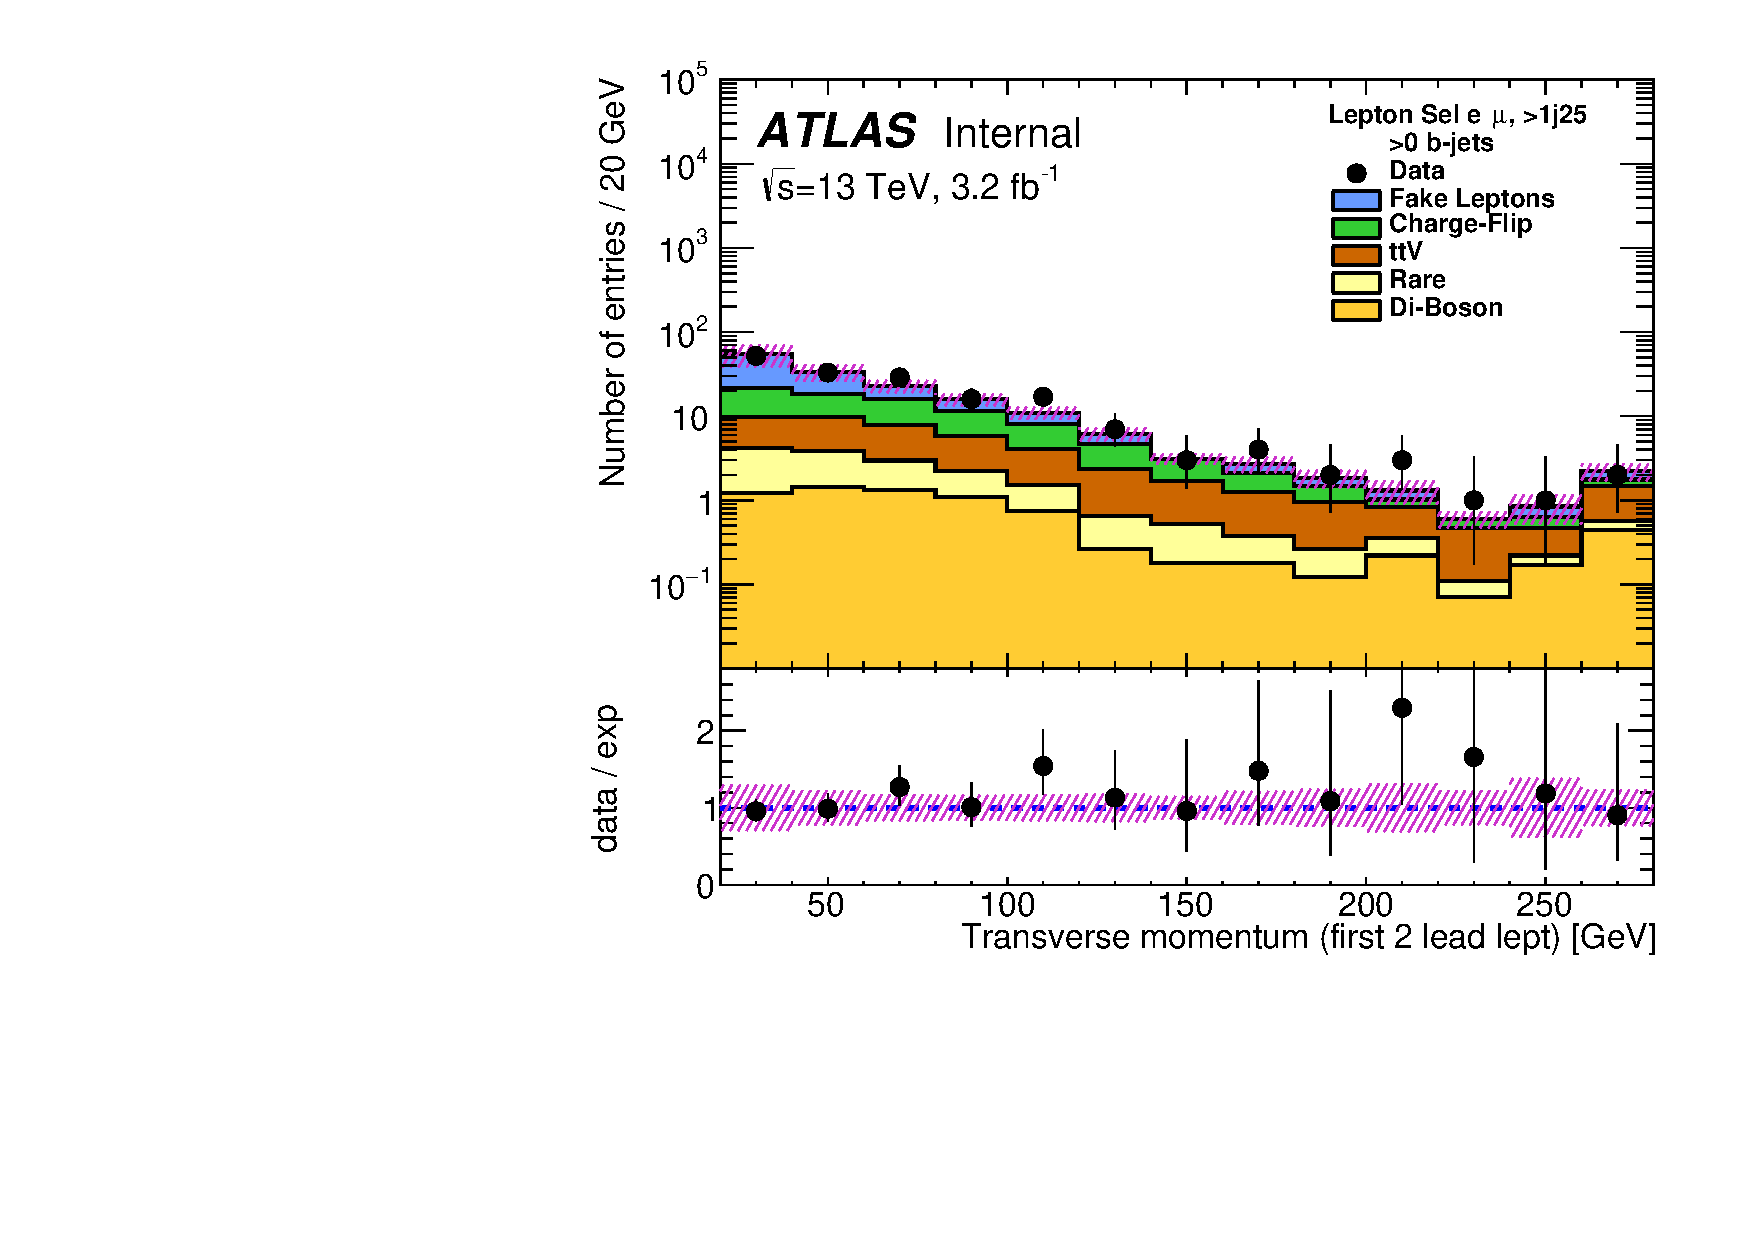
\includegraphics[width=0.45\textwidth]{BKG/validationPLots/PTLEP_EM_LEP}
}
\subfigure{
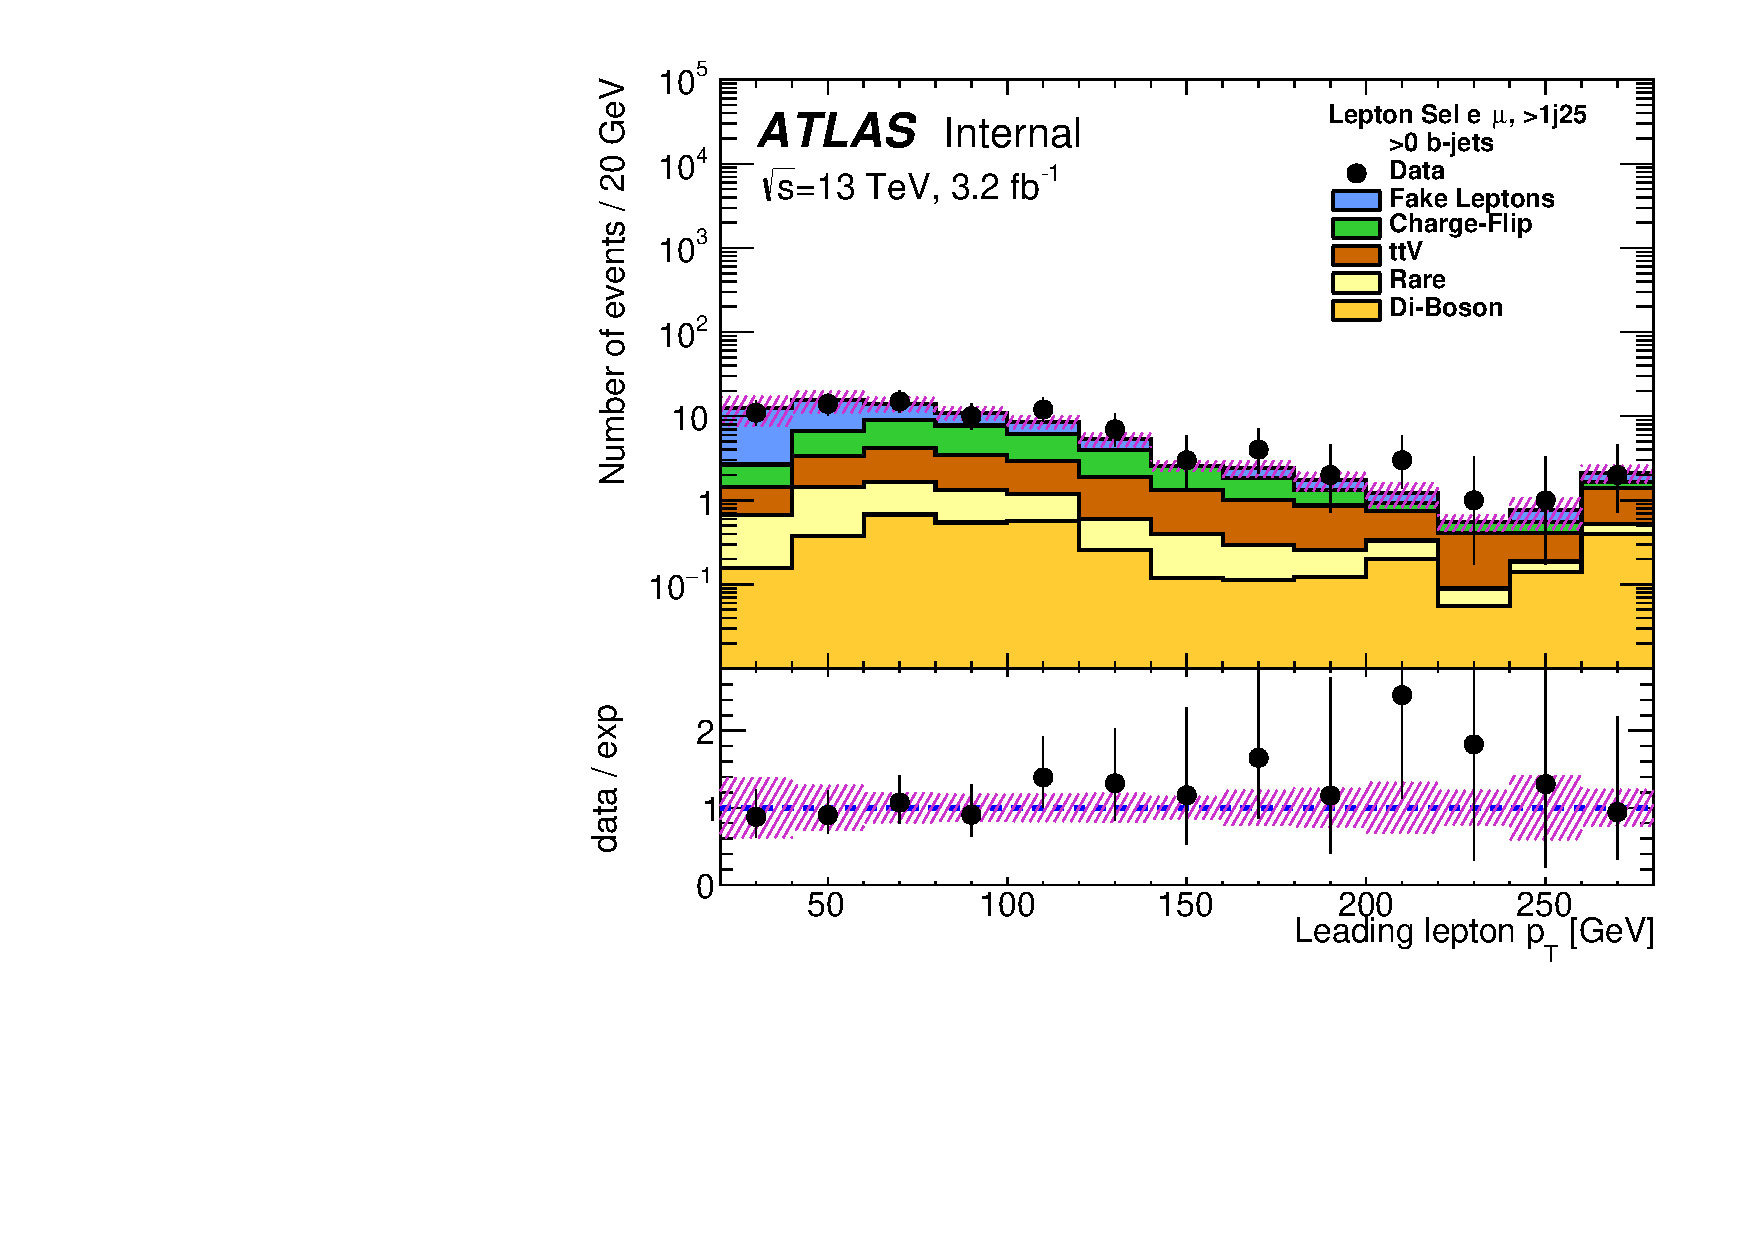
\includegraphics[width=0.45\textwidth]{BKG/validationPLots/PTLEP_EM_LEAD}
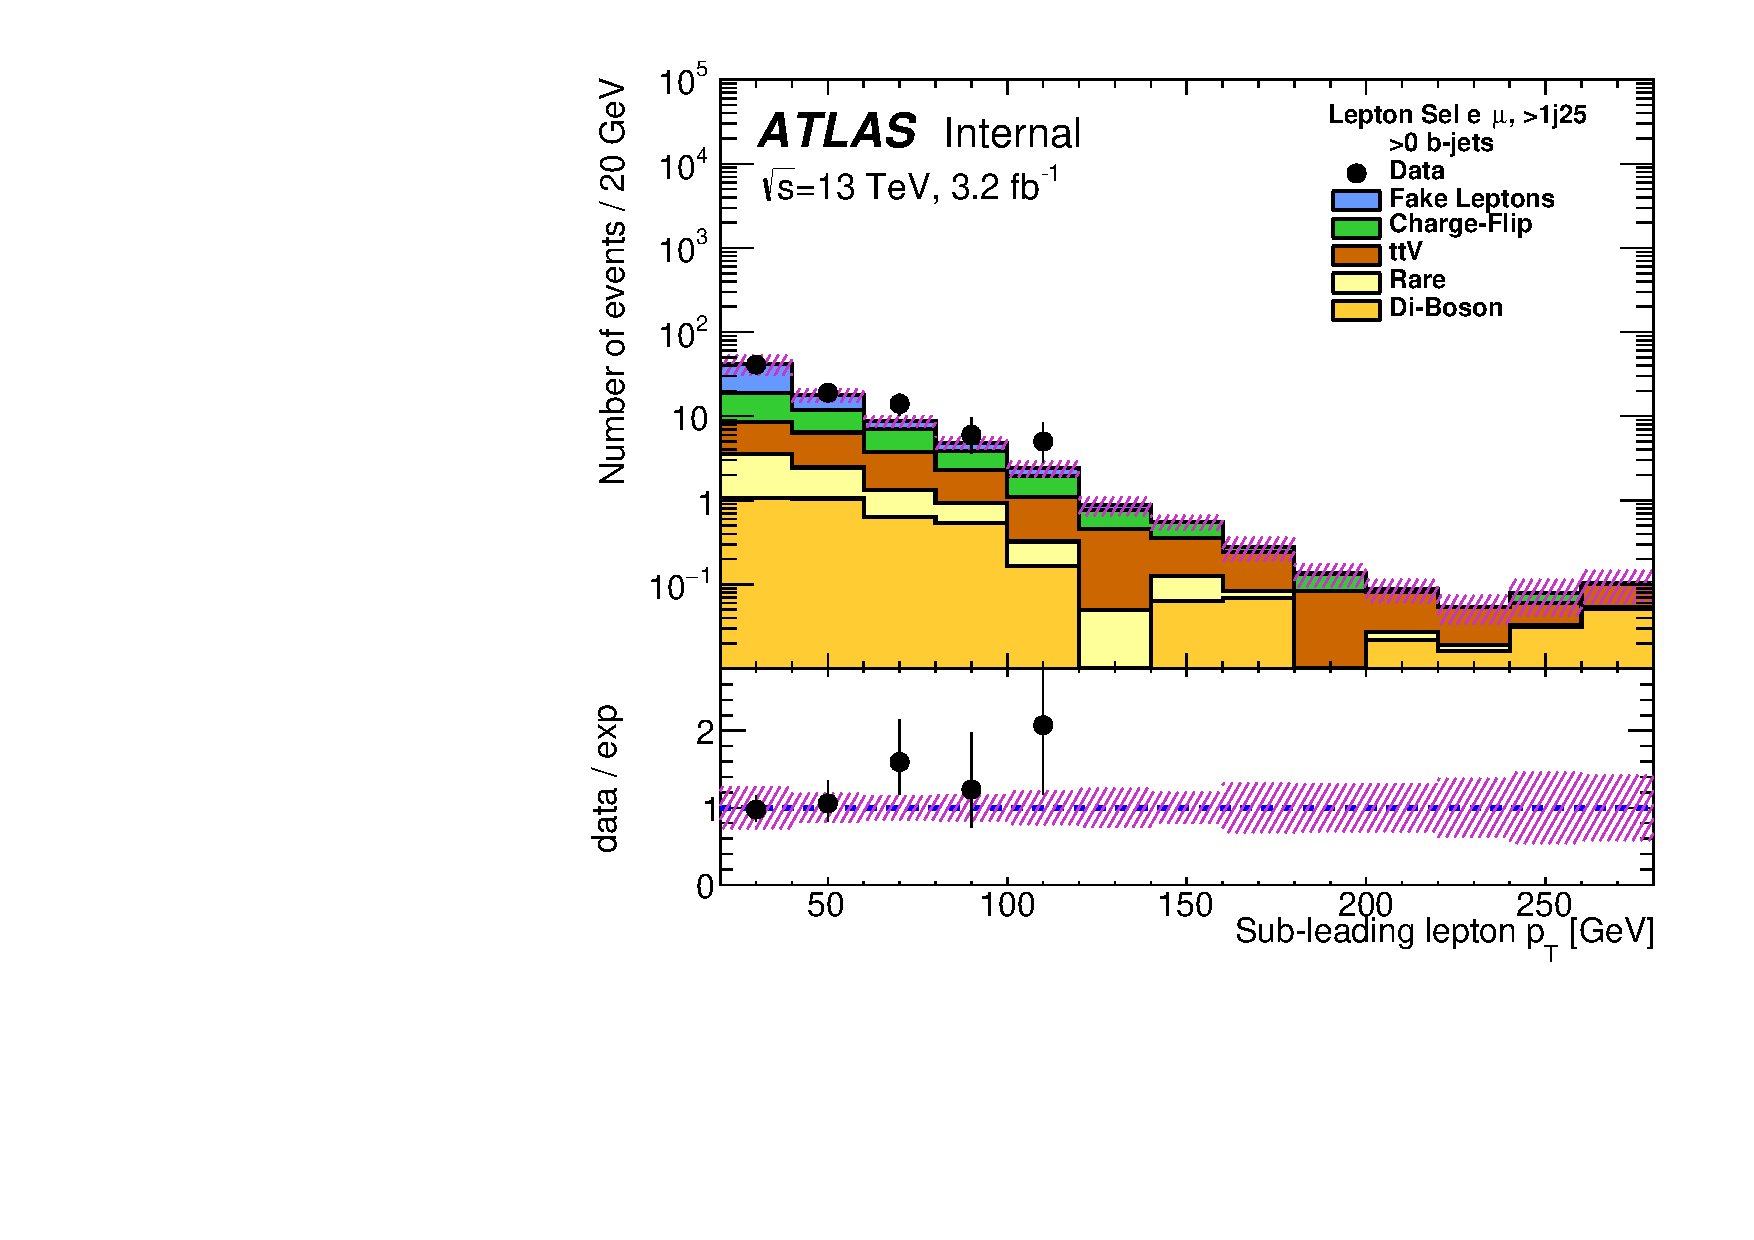
\includegraphics[width=0.45\textwidth]{BKG/validationPLots/PTLEP_EM_SUBLEAD}
}
\caption{$e\mu$ channel, \met $>$ 60\GeV and $N_{jets}^{25}$~$\ge$2: Distributions of  jet multiplicity (\pt~$>$~25~GeV) (top-left) and $b$-jet multiplicity (\pt~$>$~20~GeV) (top-right) after lepton selection, and of \mt (middle-left), selected leptons \pt (middle-right), leading lepton \pt (bottom-left) and subleading lepton \pt (bottom-right) after lepton selections with at least one $b$-jet (\pt~$>$~20~GeV).}
\label{Fig:VP_em_1b_Njets_and_other}
\end{figure} 




%%%%% emu channel, ==0 b-jet
\begin{figure}[h!]
\centering
\subfigure{
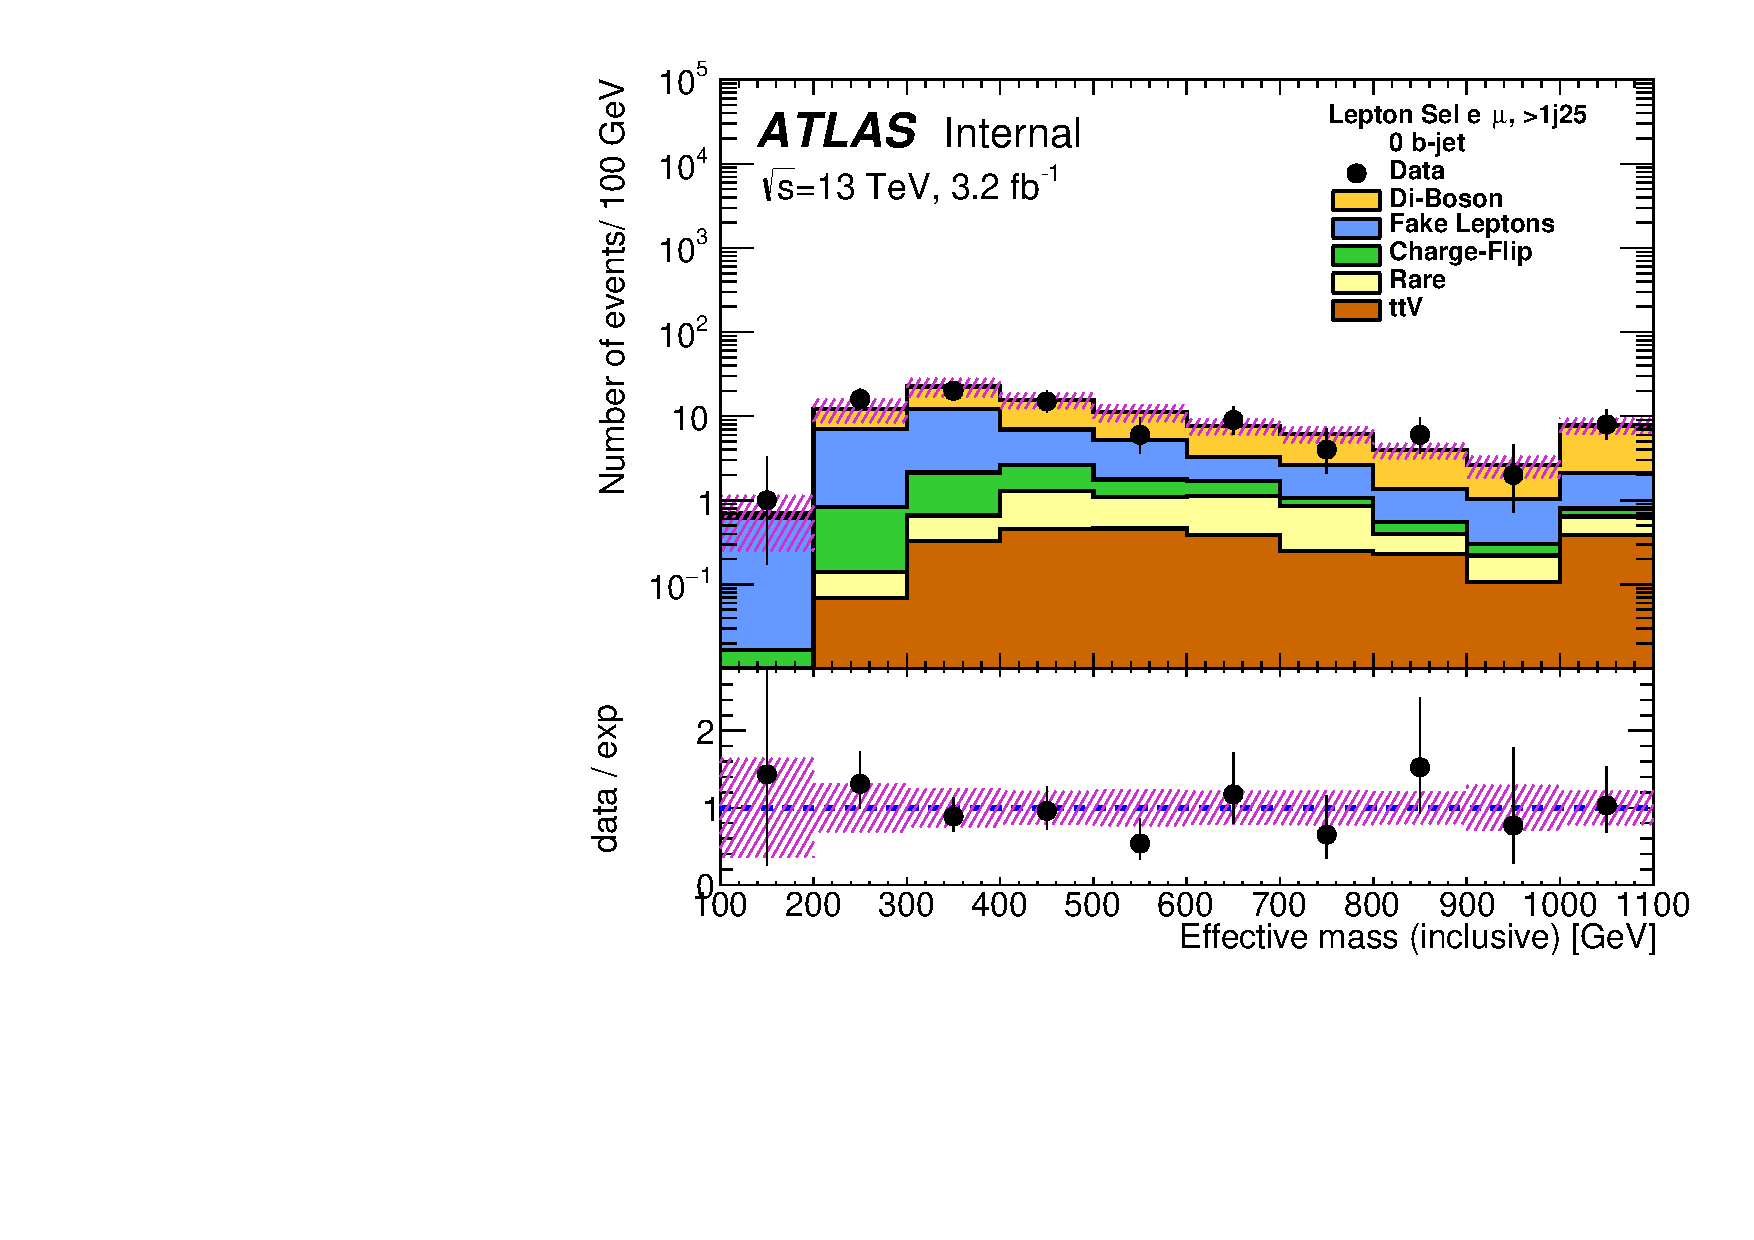
\includegraphics[width=0.5\textwidth]{BKG/validationPLots/MEFF_EM_BVETOLEP}
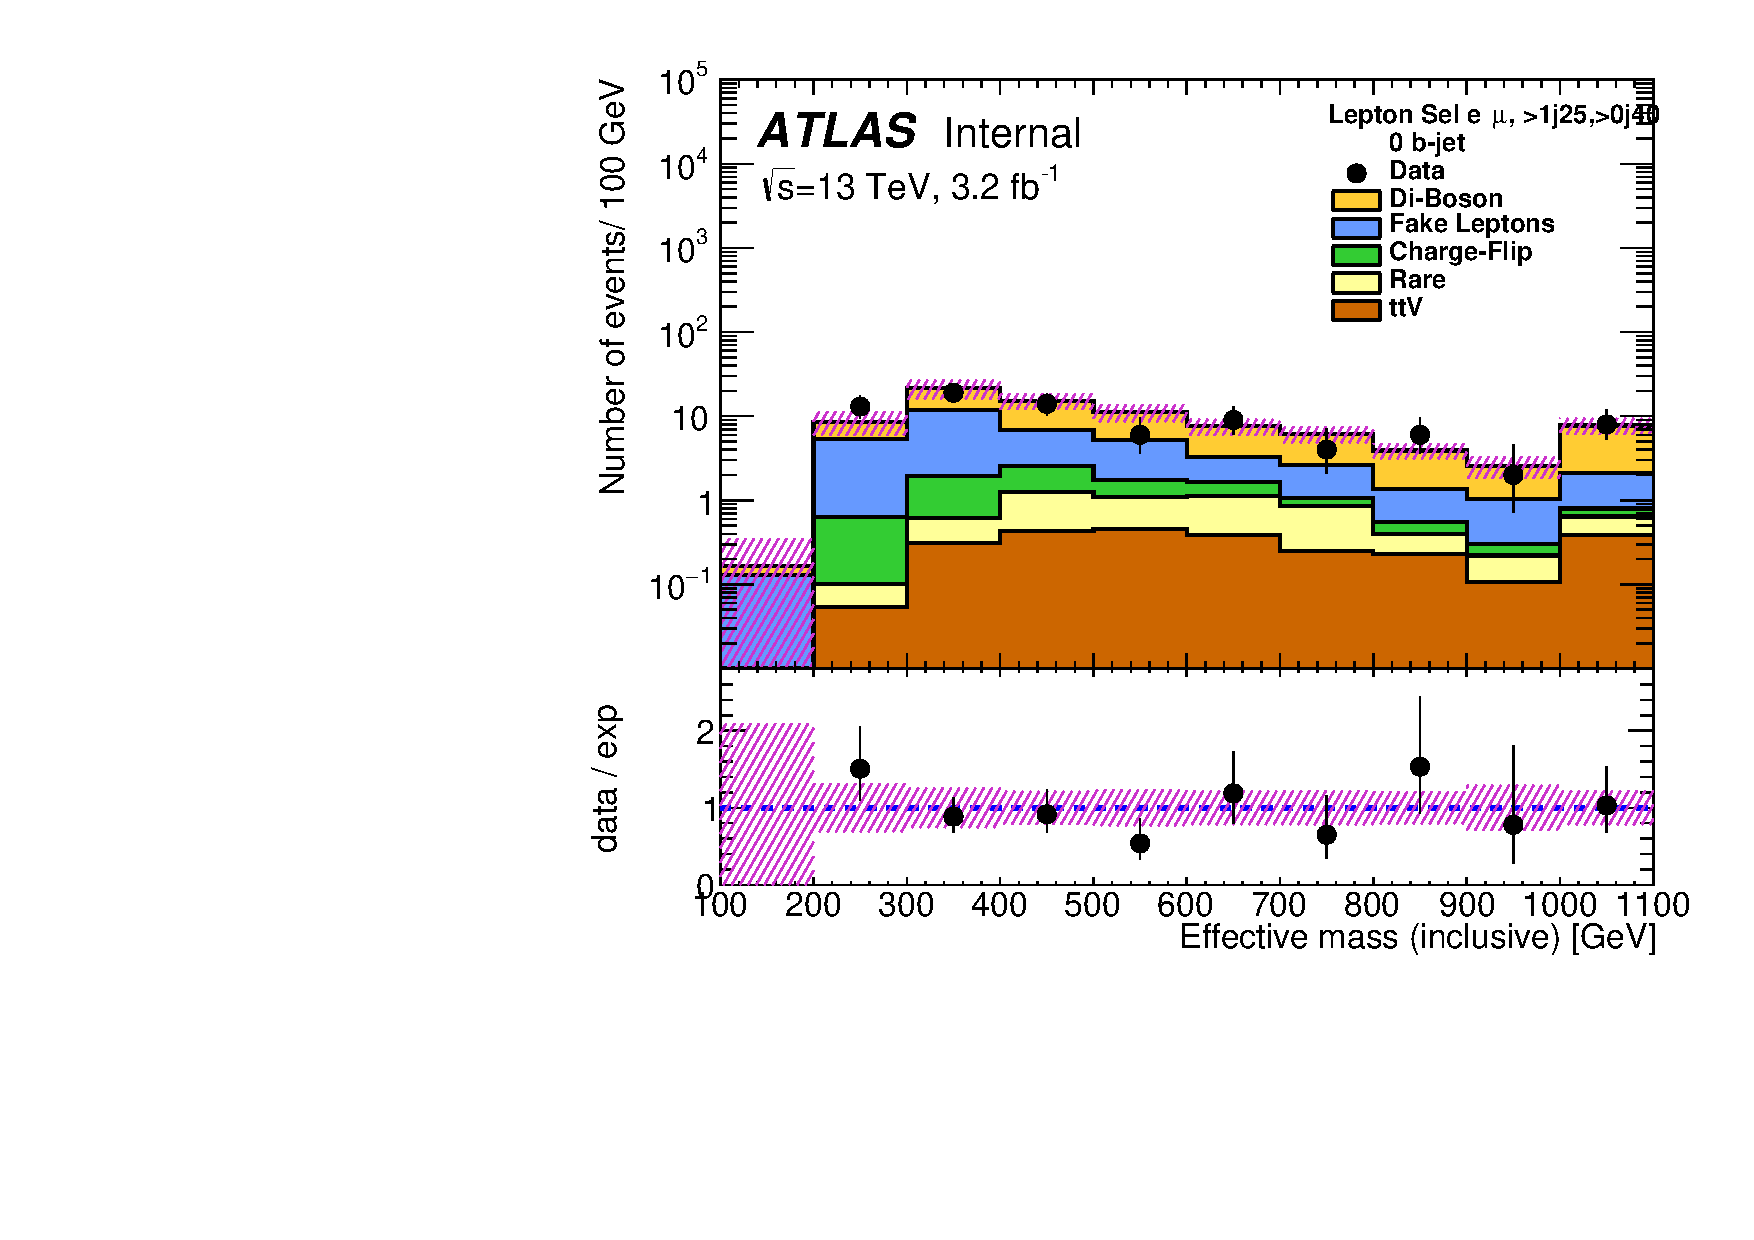
\includegraphics[width=0.5\textwidth]{BKG/validationPLots/MEFF_EM_BVETOL1JET}
}
\subfigure{
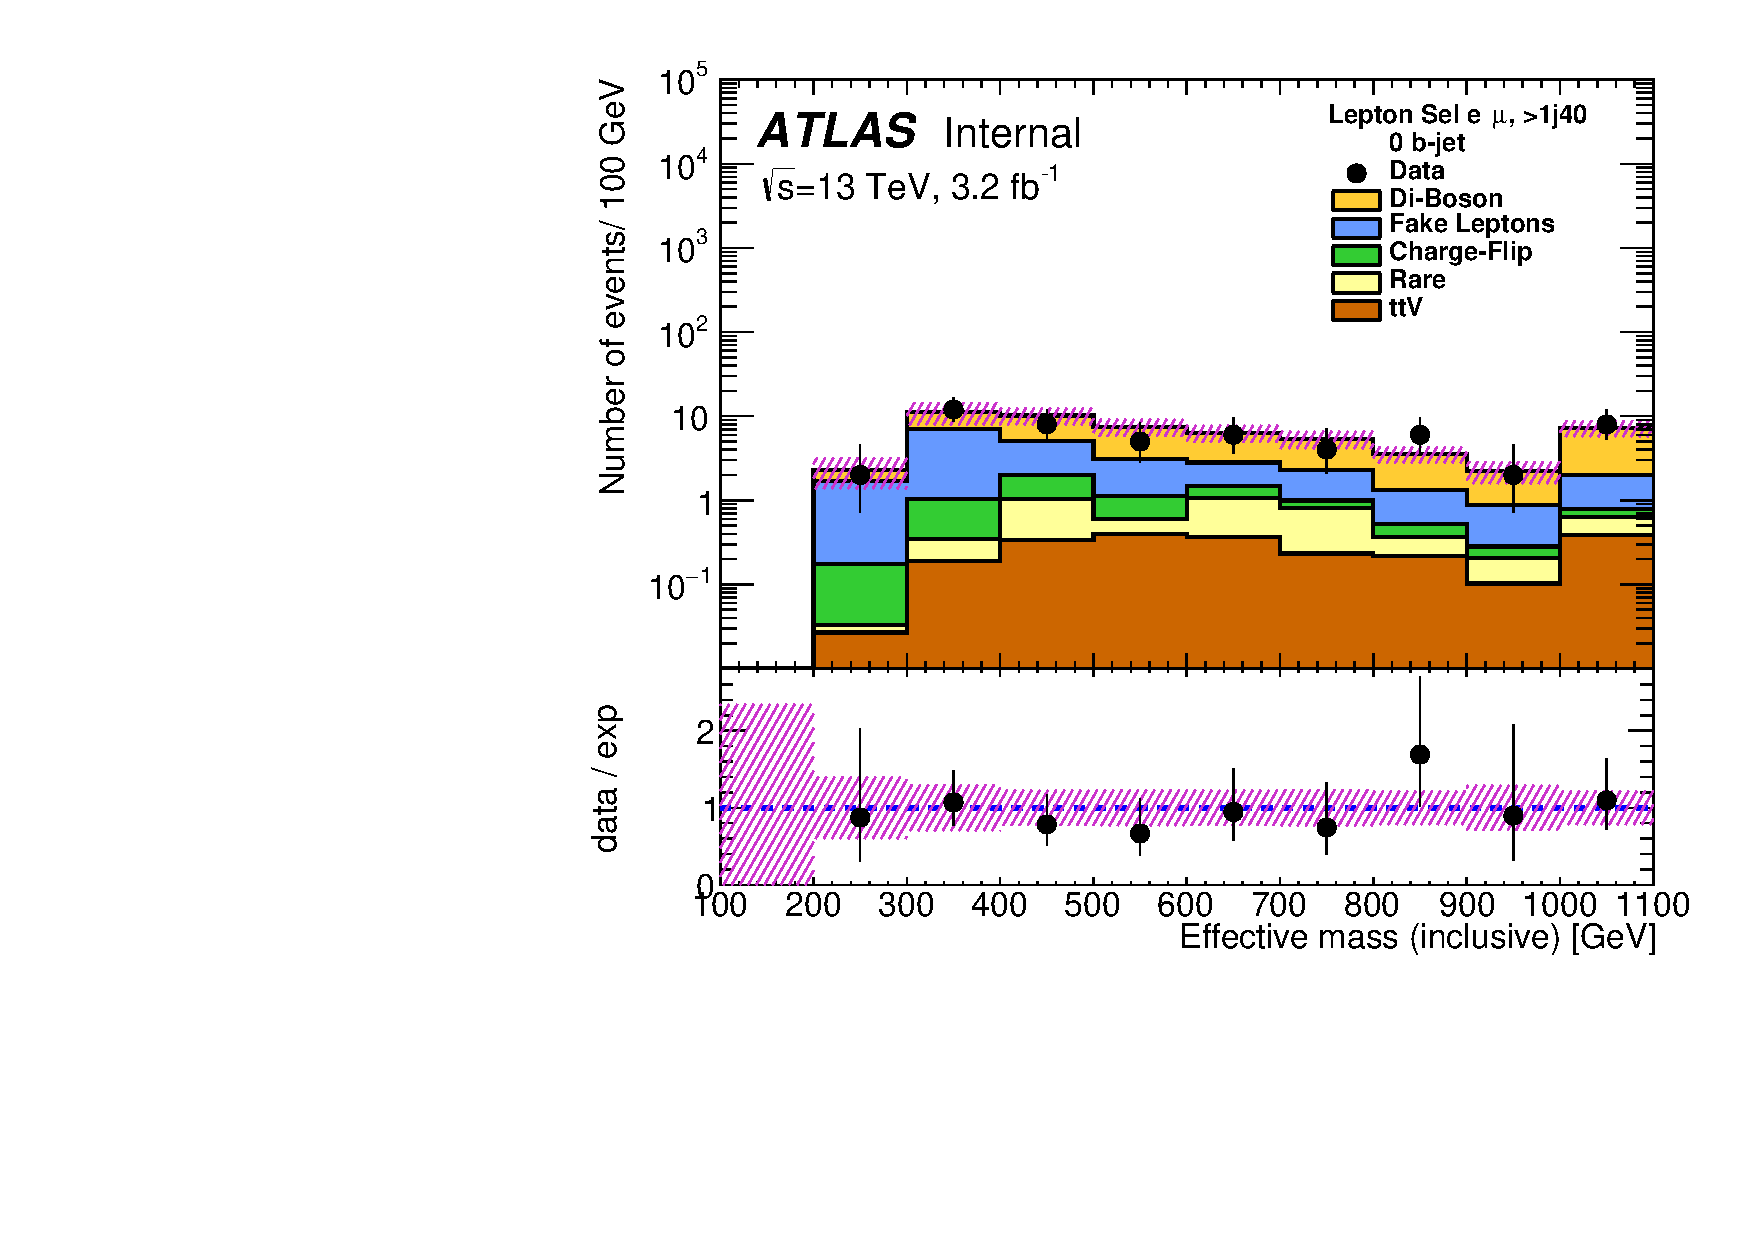
\includegraphics[width=0.5\textwidth]{BKG/validationPLots/MEFF_EM_BVETOL2JET}
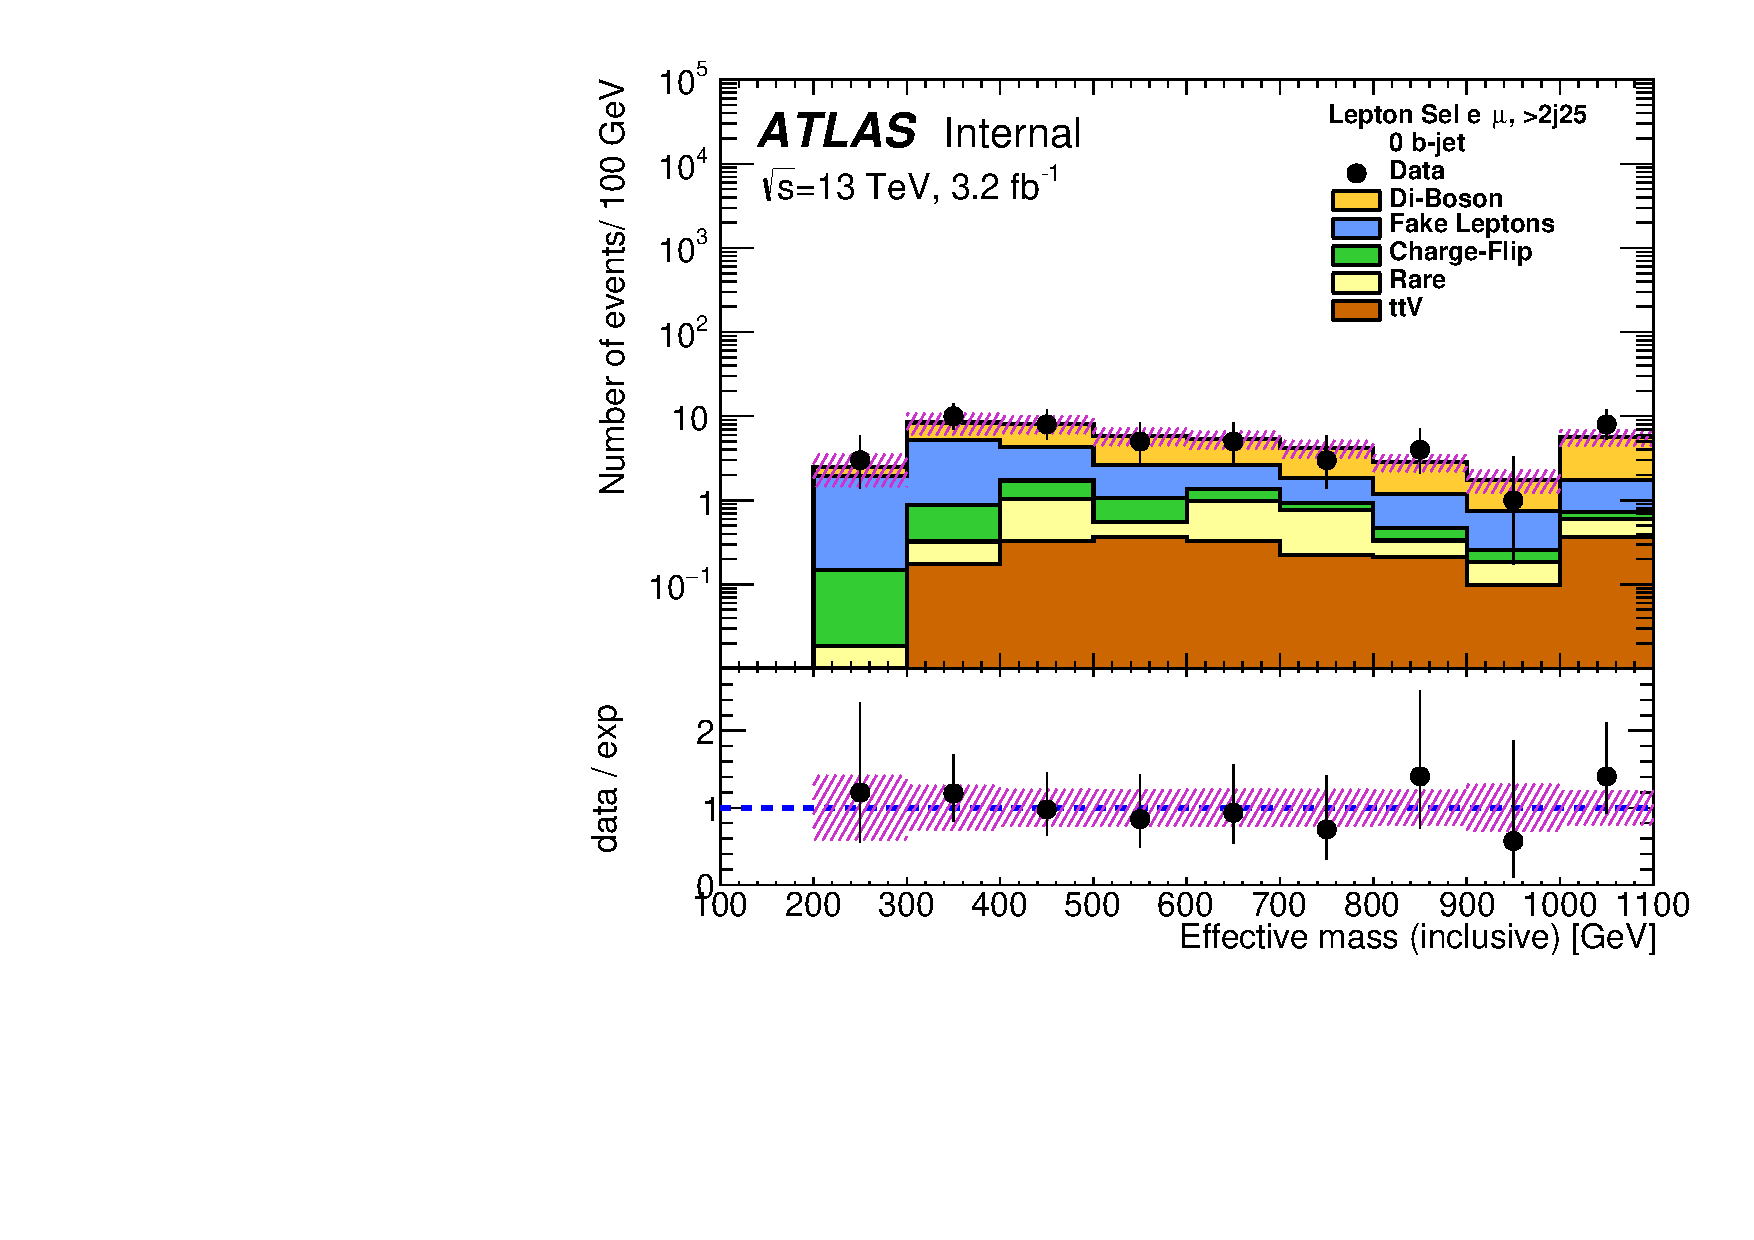
\includegraphics[width=0.5\textwidth]{BKG/validationPLots/MEFF_EM_BVETOL3JET}
}
\caption{$e\mu$ channel, \met $>$ 60\GeV and $N_{jets}^{25}$~$\ge$2: Effective mass distribution after lepton selections with a $b$-jet veto (\pt~$>$~20~GeV) and with at least 0, 1, 2 and 3 jets with \pt~$>$~40~GeV (from top-left to bottom-right).}
\label{Fig:VP_em_0b_Meff}
\end{figure}
%%
\begin{figure}[h!]
\centering
\subfigure{
\includegraphics[width=0.5\textwidth]{BKG/validationPLots/MET_EM_BVETOLEP}
\includegraphics[width=0.5\textwidth]{BKG/validationPLots/MET_EM_BVETOL1JET}
}
\subfigure{
\includegraphics[width=0.5\textwidth]{BKG/validationPLots/MET_EM_BVETOL2JET}
\includegraphics[width=0.5\textwidth]{BKG/validationPLots/MET_EM_BVETOL3JET}
}
\caption{$e\mu$ channel, \met $>$ 60\GeV and $N_{jets}^{25}$~$\ge$2: Missing transverse energy distribution after lepton selections with a $b$-jet veto (\pt~$>$~20~GeV) and with at least 0, 1, 2 and 3 jets with \pt~$>$~40~GeV (from top-left to bottom-right).}
\label{Fig:VP_em_0b_Met}
\end{figure} 
%%
\begin{figure}[h!]
\centering
\subfigure{
\includegraphics[width=0.5\textwidth]{BKG/validationPLots/MT_EM_BVETOLEP}
\includegraphics[width=0.5\textwidth]{BKG/validationPLots/PTLEP_EM_BVETOLEP}
}
\subfigure{
\includegraphics[width=0.5\textwidth]{BKG/validationPLots/PTLEP_EM_BVETOLEAD}
\includegraphics[width=0.5\textwidth]{BKG/validationPLots/PTLEP_EM_BVETOSUBLEAD}
}
\caption{$e\mu$ channel, \met $>$ 60\GeV and $N_{jets}^{25}$~$\ge$2: Distributions of \mt (top-left), selected leptons \pt (top-right), leading lepton \pt (bottom-left) and subleading lepton \pt (bottom-right) after lepton selections with with a $b$-jet veto (\pt~$>$~20~GeV).}
\label{Fig:VP_em_0b_Njets_and_other}
\end{figure} 

\FloatBarrier


%%%%% mumu channel, >= 1 b-jet
\begin{figure}[h!]
\centering
\subfigure{
\includegraphics[width=0.5\textwidth]{BKG/validationPLots/MEFF_MM_LEP}
\includegraphics[width=0.5\textwidth]{BKG/validationPLots/MEFF_MM_L1JET}
}
\subfigure{
\includegraphics[width=0.5\textwidth]{BKG/validationPLots/MEFF_MM_L2JET}
\includegraphics[width=0.5\textwidth]{BKG/validationPLots/MEFF_MM_L3JET}
}
\caption{$\mu\mu$ channel, \met $>$ 60\GeV and $N_{jets}^{25}$~$\ge$2: Effective mass distribution after lepton selections with a $b$-jet veto (\pt~$>$~20~GeV) and with at least 0, 1, 2 and 3 jets with \pt~$>$~40~GeV (from top-left to bottom-right).}
\label{Fig:VP_mm_1b_Meff}
\end{figure}
%%
\begin{figure}[h!]
\centering
\subfigure{
\includegraphics[width=0.5\textwidth]{BKG/validationPLots/MET_MM_LEP}
\includegraphics[width=0.5\textwidth]{BKG/validationPLots/MET_MM_L1JET}
}
\subfigure{
\includegraphics[width=0.5\textwidth]{BKG/validationPLots/MET_MM_L2JET}
\includegraphics[width=0.5\textwidth]{BKG/validationPLots/MET_MM_L3JET}
}
\caption{$\mu\mu$ channel, \met $>$ 60\GeV and $N_{jets}^{25}$~$\ge$2: Missing transverse energy distribution after lepton selections with a $b$-jet veto (\pt~$>$~20~GeV) and with at least 0, 1, 2 and 3 jets with \pt~$>$~40~GeV (from top-left to bottom-right).}
\label{Fig:VP_mm_1b_Met}
\end{figure}
%%
\begin{figure}[h!]
\centering
\subfigure{
\includegraphics[width=0.45\textwidth]{BKG/validationPLots/NJETS40_MM_LEP}
\includegraphics[width=0.45\textwidth]{BKG/validationPLots/NBJETS20_MM_LEP}
}
\subfigure{
\includegraphics[width=0.45\textwidth]{BKG/validationPLots/MT_MM_LEP}
\includegraphics[width=0.45\textwidth]{BKG/validationPLots/PTLEP_MM_LEP}
}
\subfigure{
\includegraphics[width=0.45\textwidth]{BKG/validationPLots/PTLEP_MM_LEAD}
\includegraphics[width=0.45\textwidth]{BKG/validationPLots/PTLEP_MM_SUBLEAD}
}
\caption{$\mu\mu$ channel, \met $>$ 60\GeV and $N_{jets}^{25}$~$\ge$2: Distributions of  jet multiplicity (\pt~$>$~25~GeV) (top-left) and $b$-jet multiplicity (\pt~$>$~20~GeV) (top-right) after lepton selection, and of \mt (middle-left), selected leptons \pt (middle-right), leading lepton \pt (bottom-left) and subleading lepton \pt (bottom-right) after lepton selections with at least one $b$-jet (\pt~$>$~20~GeV).}
\label{Fig:VP_mm_1b_Njets_and_other}
\end{figure} 



%%%%% mumu channel, ==0 b-jet
\begin{figure}[h!]
\centering
\subfigure{
\includegraphics[width=0.5\textwidth]{BKG/validationPLots/MEFF_MM_BVETOLEP}
\includegraphics[width=0.5\textwidth]{BKG/validationPLots/MEFF_MM_BVETOL1JET}
}
\subfigure{
\includegraphics[width=0.5\textwidth]{BKG/validationPLots/MEFF_MM_BVETOL2JET}
\includegraphics[width=0.5\textwidth]{BKG/validationPLots/MEFF_MM_BVETOL3JET}
}
\caption{$\mu\mu$ channel, \met $>$ 60\GeV and $N_{jets}^{25}$~$\ge$2: Effective mass distribution after lepton selections with a $b$-jet veto (\pt~$>$~20~GeV) and with at least 0, 1, 2 and 3 jets with \pt~$>$~40~GeV (from top-left to bottom-right).}
\label{Fig:VP_mm_0b_Meff}
\end{figure}
%%
\begin{figure}[h!]
\centering
\subfigure{
\includegraphics[width=0.5\textwidth]{BKG/validationPLots/MET_MM_BVETOLEP}
\includegraphics[width=0.5\textwidth]{BKG/validationPLots/MET_MM_BVETOL1JET}
}
\subfigure{
\includegraphics[width=0.5\textwidth]{BKG/validationPLots/MET_MM_BVETOL2JET}
\includegraphics[width=0.5\textwidth]{BKG/validationPLots/MET_MM_BVETOL3JET}
}
\caption{$\mu\mu$ channel, \met $>$ 60\GeV and $N_{jets}^{25}$~$\ge$2: Missing transverse energy distribution after lepton selections with a $b$-jet veto (\pt~$>$~20~GeV) and with at least 0, 1, 2 and 3 jets with \pt~$>$~40~GeV (from top-left to bottom-right).}
\label{Fig:VP_mm_0b_Met}
\end{figure}
%%
\begin{figure}[h!]
\centering
\subfigure{
\includegraphics[width=0.5\textwidth]{BKG/validationPLots/MT_MM_BVETOLEP}
\includegraphics[width=0.5\textwidth]{BKG/validationPLots/PTLEP_MM_BVETOLEP}
}
\subfigure{
\includegraphics[width=0.5\textwidth]{BKG/validationPLots/PTLEP_MM_BVETOLEAD}
\includegraphics[width=0.5\textwidth]{BKG/validationPLots/PTLEP_MM_BVETOSUBLEAD}
}
\caption{$\mu\mu$ channel, \met $>$ 60\GeV and $N_{jets}^{25}$~$\ge$2: Distributions of \mt (top-left), selected leptons \pt (top-right), leading lepton \pt (bottom-left) and subleading lepton \pt (bottom-right) after lepton selections with with a $b$-jet veto (\pt~$>$~20~GeV).}
\label{Fig:VP_mm_0b_Njets_and_other}
\end{figure} 


%%%%%%%%%%%%%%%% 3 leptons %%%%%%%%%%%%%%%%%%%%%
\clearpage
\begin{figure}[h!]
\centering
\subfigure{
\includegraphics[width=0.5\textwidth]{BKG/validationPLots/NLEP20_EE_LEP}
\includegraphics[width=0.5\textwidth]{BKG/validationPLots/NLEP20_EM_LEP}
}
\subfigure{
\includegraphics[width=0.5\textwidth]{BKG/validationPLots/NLEP20_MM_LEP}}
\caption{\met $>$ 60\GeV and $N_{jets}^{25}$~$\ge$2 : Number of leptons distribution after lepton selection in $ee$ (left), $e\mu$ (middle) and $\mu\mu$ (right) channels.}
\label{Fig:VP_Nlep_3Lep}
\end{figure}
%%
\clearpage
\begin{figure}[h!]
\centering
\subfigure{
\includegraphics[width=0.5\textwidth]{BKG/validationPLots/PTLEP_EE_THIRDLEAD}
\includegraphics[width=0.5\textwidth]{BKG/validationPLots/PTLEP_EE_BVETOTHIRDLEAD}
}
\subfigure{
\includegraphics[width=0.5\textwidth]{BKG/validationPLots/PTLEP_EM_THIRDLEAD}
\includegraphics[width=0.5\textwidth]{BKG/validationPLots/PTLEP_EM_BVETOTHIRDLEAD}
}
\subfigure{
\includegraphics[width=0.5\textwidth]{BKG/validationPLots/PTLEP_MM_THIRDLEAD}
\includegraphics[width=0.5\textwidth]{BKG/validationPLots/PTLEP_MM_BVETOTHIRDLEAD}
}
\caption{3leptons, \met $>$ 60\GeV and $N_{jets}^{25}$~$\ge$2 : Third lepton \pt distribution after lepton selection with at least one $b$-jet (left) and 0 $b$-jets (right). Results are shown in $ee$ (left), $e\mu$ (middle) and $\mu\mu$ (right) channels.}
\label{Fig:VP_PtLep_3Lep}
\end{figure} 
  

\FloatBarrier

%%%%%%%%%%%%%%%%%%%%%%%%
%\subsection{Validation of background estimates with 3 $b$-jets}
%\label{sec:bkg_VP_3b_MC}
%
%We have a signal region, SR3b, which requires $\ge$3 $b$-jets of \pt~$>$~20~GeV, the background for which is determined both by data-driven estimates and Monte Carlo samples. In order to demonstrate that the $b$-tagging efficiencies in data are well modeled by Monte Carlo, including the mistag rate of light flavor jets, a higher statistics opposite-sign dilepton region with $\ge$3 $b$-jets is considered. Compared to the Monte Carlo samples used to obtain the validation plots from Section~\ref{sec:bkg_VP_DD_estimates}, extra samples have been considered to model the \ttbar, single top and $Z$+jets backgrounds.The (low) fake lepton background is estimated using Monte Carlo.
%
%Distributions were made with $b$-tagging calibration weights and shown in Figures~\ref{fig:3b_OS_MC_estim:meff_met}-\ref{fig:3b_OS_MC_estim:pt_jet}. 
%Generally the agreement between data and MC is rather good, although the statistics is very low. 
%
%% Distributions were made both with (Figure~\ref{}) and without (Figure~\ref{}) b-tagging calibration weights. The first important observation is that little changes between the two figures – thus we do not appear to be vulnerable to problems in the calibration that are known to exist for some samples. Further, it is seen that agreement is generally good. There are some kinematic discrepancies at large ** multiplicity, where the background over-predicts the data, however these can be safely ignored, as they are most likely due to issues in the ** Monte Carlo sample, which is not required for estimating the same-sign background. It is particularly encouraging that the b-jet pT distributions appear to agree well for low through to high \pt, and the b-jet multiplicity distribution indicates excellent agreement for exactly 3 b-jets.
%
%\begin{figure}[h!]
%\centering
%\subfigure{
%\includegraphics[width=0.5\textwidth]{fig_3b_OS_MC_Estim/MEFF_afterlepton_3b_0_physics}
%\includegraphics[width=0.5\textwidth]{fig_3b_OS_MC_Estim/MET_afterlepton_3b_0_physics}
%}
%\subfigure{
%\includegraphics[width=0.5\textwidth]{fig_3b_OS_MC_Estim/PTLEP1_afterlepton_3b_0_physics}
%\includegraphics[width=0.5\textwidth]{fig_3b_OS_MC_Estim/PTLEP2_afterlepton_3b_0_physics}
%}
%\caption{Distributions of effective mass (top-left), missing transverse momentum (top-right), leading lepton \pt (bottom-left) and subleading lepton \pt (bottom-right) after opposite-sign leptons selection with at least three $b$-jets. Only luminosity and MC statistical uncertainties are included.}
%\label{fig:3b_OS_MC_estim:meff_met}
%\end{figure} 
%%%
%\begin{figure}[h!]
%\centering
%\subfigure{
%\includegraphics[width=0.5\textwidth]{fig_3b_OS_MC_Estim/NLEP_afterlepton_3b_0_physics}
%\includegraphics[width=0.5\textwidth]{fig_3b_OS_MC_Estim/NBJET70_20_afterlepton_3b_0_physics}
%}
%\subfigure{
%\includegraphics[width=0.5\textwidth]{fig_3b_OS_MC_Estim/NJET30_afterlepton_3b_0_physics}
%\includegraphics[width=0.5\textwidth]{fig_3b_OS_MC_Estim/NJET40_afterlepton_3b_0_physics}
%}
%\caption{Distributions of number of leptons (top-left), number of $b$-jets with \pt~$>$~20~GeV (top-right), number of jets with \pt~$>$~30~GeV (bottom-left) and number of jets with \pt~$>$~40~GeV (bottom-right) after opposite-sign leptons selection with at least three $b$-jets. Only luminosity and MC statistical uncertainties are included.}
%\label{fig:3b_OS_MC_estim:nlep_njets}
%\end{figure} 
%%%
%\begin{figure}[h!]
%\centering
%\subfigure{
%\includegraphics[width=0.5\textwidth]{fig_3b_OS_MC_Estim/PTJET1_afterlepton_3b_0_physics}
%\includegraphics[width=0.5\textwidth]{fig_3b_OS_MC_Estim/PTBJET70_1_afterlepton_3b_0_physics}
%}
%\subfigure{
%\includegraphics[width=0.5\textwidth]{fig_3b_OS_MC_Estim/PTBJET70_2_afterlepton_3b_0_physics}
%\includegraphics[width=0.5\textwidth]{fig_3b_OS_MC_Estim/PTBJET70_3_afterlepton_3b_0_physics}
%}
%\caption{Distributions of number of leading jet \pt (top-right), leading $b$-jet \pt (top-left), subleading $b$-jet \pt (bottom-left) and third $b$-jet \pt (bottom-right) after opposite-sign leptons selection with at least three $b$-jets. Only luminosity and MC statistical uncertainties are included.}
%\label{fig:3b_OS_MC_estim:pt_jet}
%\end{figure} 
%

   
%%%%%%%%%%%%%%%%%%%%%%%
\subsection {Validation regions}
\label{sec:bkg_VR}
In this section the validation regions (VR) defined to check the prompt SS background are described. The observed number of data events and the corresponding background estimation are also shown at the end of the section. The definition of these validation regions is 
summarized in Table~\ref{tab:VRdef} and is detailed below. 
In all validation regions the signal regions defined in Table~\ref{tab:SRdef3} are vetoed to minimize the signal contamination and any overlap between the regions. As a \ttbar\ + $V$ validation region is very sensitive to models including third generation squarks (like direct sbottom pair production) we choose to veto any event passing SR2b defined in Table~\ref{tab:SRdefAux}. Given the excess observed in Run-1, we choose to veto also any event passing the SR3L3b (Table~\ref{tab:SRdefAux}) selection. The latter cut is applied in all validation regions. The ``signal removal'' cuts are shown with ``!SR'' in the tables.


\begin{table}[htb!]
\caption{Summary of the event selection in the validation regions. 
Requirements are placed on the number of signal leptons ($N_{\rm{lept}}^{\rm{signal}}$) and candidate leptons ($N_{\rm{lept}}^{\rm{cand}}$), 
%the number of jets with $\pt>\SI{25}{GeV}$ $\left(N_{\rm{jets}}^{25}\right)$ or the number of $b$-jets $\left(N_{b\rm{ jets}}^{20}\right)$. 
the number of jets with $\pt>\SI{25}{GeV}$ ($N_{\rm{jets}}^{25}$) or the number of $b$-jets with $\pt>\SI{20}{GeV}$ ($N_{b\rm{-jets}}^{20}$). 
The three leading \pt leptons are referred to as $\ell_{1,2,3}$ with decreasing \pt and the two leading jets as $j_{1,2}$.
Additional requirements are set on the invariant mass of the two leading electrons $m_{ee}$, 
the presence of SS leptons or a pair of same-flavour opposite-sign leptons (SFOS) and its invariant mass $m_\text{SFOS}$. 
}
\hspace{0.5cm}
\def\arraystretch{1.1}
\label{tab:VRdef}
\centering
\resizebox{\textwidth}{!}
{\small
\begin{tabular}{c|c|c|c|c|c|l}
\hline 
\hline    
          &  $N_{\rm{lept}}^{\rm{signal}}$ ($N_{\rm{lept}}^{\rm{cand}}$)   & $N_{b\rm{-jets}}^{20}$  &  $N_{\rm{jets}}^{25}$  & \met\ [GeV] & \meff\ [GeV]  & Other \\
\hline\hline
VR-WW   & =2 (=2) &  =0  &  $\geq$2 & 35--200  & 300--900 & $m(j_1 j_2)>500$~GeV\\
          & =1 SS pair    &      &             &         &         & $\pt(j_2)>40$~GeV\\
          &      &      &             &         &         & $\pt(\ell_2)>30$~GeV\\
%          &      &      &             &         &         & $|\eta(e_{1,2})|<1.37$\\
          &      &      &             &         &         & veto $80<m_{ee}<100$~GeV \\\hline
VR-WZ     & =3 (=3) &  =0  &  1--3     & 30--200  & $<$900 & $\pt(\ell_3)>30$~GeV \\ \hline
VR-ttV    &$\geq$2 (-) &$\geq$2&  $\geq$5 ($e^\pm e^\pm$,$e^\pm \mu^\pm$) & 20--200  & 200--900 & $\pt(\ell_2)>25$~GeV\\
          & $\geq$1 SS pair  &         &  $\geq$3 ($\mu^\pm \mu^\pm$)             &          &         & veto $\{\met>125$ and $\meff>\SI{650}{GeV}\}$\\ \hline %$|\eta(e_{1,2})|<1.37$\\ \hline
VR-ttZ    &$\geq$3 (-) & $\geq$1 & $\geq$4 ($=$1 $b$-jet)         & 20--150  & 100--900 & $\pt(\ell_2)>25$~GeV\\
          &$\geq$1 SFOS pair &         & $\geq$3 ($\geq$2 $b$-jets) &           &     & $\pt(\ell_3)>20$~GeV (if $e$)\\
%          &        &         &                           &          &         & $|\eta(e_{1,2})|<1.37$ \\
          &        &         &                           &          &         & $80<m_\text{SFOS}<100$~GeV \\
\hline\hline
All VRs & \multicolumn{6}{c}{Veto events belonging to any SR, or if $\ell_1$ or $\ell_2$ is an electron with $|\eta|>1.37$ (except in VR-WZ)}\\
\hline\hline
\end{tabular}
}
\end{table}


%%
\par{\bf \ttbar\ + $V$ background validation\\}
To validate the \ttbar\ + $Z$ and \ttbar\ + $W$ background estimation, several tentative regions defined with at least 1 or 2 $b$-jets in the event are optimized. Given the low statistics expected for 2-4\ifb no \ttbar\ + $W$ validation region could be proposed. A \ttbar\ + $Z$ enriched validation region ($ttZ$ 1bIncl) is defined in Table~\ref{tab:ttZ_VR} as a combination of two orthogonal regions, ``==1 $b$'' ($ttZ$ 1bExcl) and ``$\ge$2 $b$-jets'' ($ttZ$ 2bIncl). Beside the $b$-jet(s), at least three energetic signal leptons and at least 3 (4) soft jets (\pt~$>$~25~\GeV) are required in the event. A cut on the $Z$ boson mass ($80 < m^{SFOS}_{\ell\ell} < 100$~GeV) ensures a high purity, rejecting multi-boson processes. The fake lepton background is reduced with minimum cuts on \met\ and \meff, and with tight constraints on the electron acceptance ($|\eta|_{e1,2}$~$<$~1.37). The reached purity is 70\%. 

A second \ttbar\ + $V$ validation region ($ttV$ 2bIncl) is defined in Table~\ref{tab:ttV_VR} with at least two $b$-jets and at least two energetic signal leptons. The highest purity is found with at least five soft jets in the $ee$ and $e\mu$ channels, and at least three soft jets in the $\mu\mu$ channel. Cuts on \meff\  and electron acceptance ($|\eta|_{e1,2}$~$<$~1.37) are applied to reduce the detector background. The obtained purity is 50\%. 

In both validation regions the signal contamination is reduced by vetoing the signal regions (including SR2b and SR3L3b) and by 
applying upper cuts on \meff\ (900~GeV) and \met\ (150-200~GeV). 
Note that the \meff\ cut can be tighten to further decrease the SUSY contamination from models like direct sbottom. Using DC14 MC samples, in \ttbar\ + $Z$ VR it was found to be up to 27$\%$ when the direct-sbottom model was considered (sbottom mass of 550 \GeV) and up to 20$\%$ for direct squark (2 step) via sleptons with $W/Z$ bosons in the cascade decay, otherwise smaller than 10$\%$.   

\begin{table}[htb!]
\caption{\ttbar\ + $Z$ validation region definition ($ttZ$ 1bIncl = $ttZ$ 1bExcl || $ttZ$ 2bIncl).}
\label{tab:ttZ_VR}
\begin{center}
 \resizebox{\textwidth}{!}{
    \begin{tabular}{|c|c|c|c|}
      \hline 
      \hline
     VR& $ N_{lept}^{signal}$ & $N_{b-jets}^{20}$   & Other variables \\ \hline
    $ttZ$ 1bExcl & $\ge$3, \pt : (l1, l2, e3 ($\mu3$)) = (25, 25, 20 (10)) GeV & ==1  & 20 $<$ \met $<$ 150 \GeV, 100 $<$ \meff $<$ 900 \GeV,  \\
   &  & & $N_{jets}^{25}$ $\ge$ 4, $|\eta|_{e1,2}$~$<$~1.37, $80 < m^{SFOS}_{\ell\ell} < 100$~GeV, !SR\\\hline
    $ttZ$ 2bIncl& $\ge$3, \pt : (l1, l2, e3 ($\mu3$)) = (25, 25, 20 (10)) GeV & $\ge$2  & 20 $<$ \met $<$ 150 \GeV, 100 $<$ \meff $<$ 900 \GeV, \\
   &  & & $N_{jets}^{25}$ $\ge$ 3, $|\eta|_{e1,2}$~$<$~1.37, $80 < m^{SFOS}_{\ell\ell} < 100$~GeV, !SR\\\hline\hline
\end{tabular}}
\end{center}
\end{table}
%%
\begin{table}[htb!]
\caption{\ttbar\ + $V$ validation region definition ($ttV$ 2bIncl). }
\label{tab:ttV_VR}
\begin{center}
\resizebox{\textwidth}{!}{
    \begin{tabular}{|c|c|c|c|}
      \hline 
      \hline
     VR& $ N_{lept}^{signal}$ & $N_{b-jets}^{20}$     & Other variables \\ \hline
    $ttV$ 2bIncl& $\ge 2$, \pt : (l1, l2, l3) = (25, 25, 10) GeV & $\ge$2  & 20 $<$ \met $<$ 200 \GeV, 200 $<$ \meff $<$ 900 \GeV, $|\eta|_{e1,2}$~$<$~1.37, \\
   &  && $N_{jets}^{25}$ $\ge$ 5 in $ee$ and $e\mu$, $N_{jets}^{25}$ $\ge$ 3 in $\mu\mu$ channels, !SR\\\hline	\hline
\end{tabular}}
\end{center}
\end{table}

%%
\par{\bf $WZ$ + jets validation region\\}
Even if this type of background is minor in several of the defined signal regions, its contribution can be significant in regions with no $b$ jet requirement and three leptons. Therefore, a validation region ($WZ$1j 0bExcl) is defined as shown in Table~\ref{tab:WZ_VR}. It requires exactly three leptons and a veto on the fourth-leading baseline lepton in order to reduce the $ZZ$ background contamination. The lower cut on \met\ (30~\GeV) is mainly reducing the charge flip. At least one and at most three jets with \pt~$>$~25 \GeV are required in the event. The purity is around 81$\%$. The signal contamination was studied with DC14 samples, and it was found to be below 1$\%$.

\begin{table}[htb!]
\caption{$WZ$ + jets validation region definition ($WZ$1j 0bExcl).}
\label{tab:WZ_VR}
\begin{center}
   \resizebox{\textwidth}{!}{
    \begin{tabular}{|c|cc|c|c|}
      \hline
      \hline
     VR & $N_{lept}^{signal}$ & $N_{lept}^{baseline}$ &  $N_{b-jets}^{20}$     & Other variables \\ \hline
     $WZ$1j 0bExcl& $==$3,  \pt : (l1, l2, l3) = (30, 30, 30) GeV& $<4$  & $==$0  & 30 $<$ \met $<$ 200 \GeV, 100 $<$ \meff $<$ 900 GeV, 1 $\leq$ $N_{jets}^{25}$ $<$ 4, !SR \\\hline\hline
\end{tabular}}
\end{center} 
\end{table}

%%
\par{\bf $W^\pm W^\pm$ + jets validation region\\}
Similarly to other diboson processes, the $W^{\pm}W^{\pm}$ + jets events contribute mainly in the signal regions with no $b$ jet requirement. The defined validation region ($W^\pm W^{\pm}$mjj  0bExcl) is presented in Table~\ref{tab:WW_VR}. A cut on the invariant mass of the first two leading jets in the event is considered to remove most of the $WZ$ + jets processes. Even if it selects forward jets from VBS processes, which are not necessary populating the signal regions defined in the analysis, it gives a confidence on this type of background. No other validation region (i.e with two energetic jets) could be defined, because of the high background contamination. The reached purity is around 44\%.  The signal contamination is reduced by applying an upper cut on \met\ (200~\GeV) -- with the DC14 samples, it was found to be around 15$\%$.

\begin{table}[htb!]
\caption{$W^\pm W^\pm$ validation region definition ($W^\pm W^{\pm}$mjj  0bExcl).}
\label{tab:WW_VR}
\begin{center}
 \resizebox{\textwidth}{!}{
    \begin{tabular}{|c|cc|c|c|}
      \hline
      \hline
     VR & $N_{lept}^{signal}$ & $N_{lept}^{baseline}$ &  $N_{b-jets}^{20}$     & Other variables \\ \hline
     $W^\pm W^{\pm}$mjj 0bExcl & $==$2, \pt : (l1, l2) = (30, 30) GeV & $==2$  & $==$0  & 35 $<$ \met $<$ 200 \GeV, $80 < m^{SS}_{ee} < 100$~GeV, $m_{jj}$ $>$ 500 \GeV,\\ 
     &&&&300 $<$ \meff $<$ 900 GeV, $N_{jets}^{40}$ $\ge$ 2, $|\eta|_{e1,2}$~$<$~1.37, !SR\\\hline	 \hline
\end{tabular}}
\end{center} 
\end{table}


%%
\par{\bf Results in the validation regions with 3.2~\ifb\ of data\\}

The event yields in the defined validation regions are shown in Table~\ref{tab:Results_VR_allCh}. 
The effective mass distribution in the validation regions is shown in Figure~\ref{fig:Results_VR}. 
A comparison between the purely data driven estimation of the detector background (DD-Total) and the estimation using the MC-based method (MC-Total) is shown in Table~\ref{tab:Results_VR_allCh_Comparison}. Generally a good agreement is observed, within the uncertainties, although the ttV and ttZ regions show some tension (data excess) at the level of $1.7\sigma$. More about this excess in Appendix~\ref{appendix:ttV}.

In the plots, the prompt SS background uncertainties include the statistical component and the theoretical systematic uncertainties as described in Section~\ref{sec:syst_theo}. For the detector background estimation the uncertainties include all sources presented in section~\ref{sec:bkg}.

\begin{table}[htb!]
\caption{The numbers of observed data and expected background events for the validation regions. 
The ``Rare'' category contains the contributions from $\ttbar \ttbar$, $\ttbar t$, $\ttbar h$ and $\ttbar WW$ production. Background categories shown as ``$-$'' denote that they cannot contribute to a given region (charge flips or $W^\pm W^\pm jj$ in 3-lepton regions).}
\label{tab:Results_VR_allCh}
\begin{center}
\setlength{\tabcolsep}{0.0pc}
{\small
%%
\begin{tabular*}{\textwidth}{@{\extracolsep{\fill}}lrrrr}
\noalign{\smallskip}\hline\noalign{\smallskip}
			& $W^\pm W^\pm jj$        & $WZj$     & $t\bar t V$ & $t\bar tZ$     \\[-0.05cm]
\noalign{\smallskip}\hline\noalign{\smallskip}
%%
Observed events          & $4$       &  $82$   & $19$  & $14$             \\
\noalign{\smallskip}\hline\noalign{\smallskip}
%%
Total bkg events & $3.4 \pm 0.8$ & $98 \pm 15$ & $12.1 \pm 2.7$ & $9.7 \pm 2.5$\\
\noalign{\smallskip}\hline\noalign{\smallskip}
Fake/non-prompt leptons & $0.6 \pm 0.5$ & $8 \pm 6$ & $2.1 \pm 1.4$ & $0.6\pm 1.0$\\ % syst+stat % NB: no error on rounding 
Charge-flip & $0.26 \pm 0.05$ & $-$ & $1.14 \pm 0.15$ & $-$\\ % syst+stat
$t\bar{t}W$ & $0.05 \pm 0.03$ & $0.25 \pm 0.09$ & $2.4 \pm 0.8$ & $0.10 \pm 0.03$\\
$t\bar{t}Z$ & $0.02 \pm 0.01$ & $0.72 \pm 0.26$ & $3.9 \pm 1.3$ & $6.3 \pm 2.1$\\
$WZ$ & $1.0 \pm 0.4$ & $78 \pm 13$ & $0.19 \pm 0.10$ & $1.2 \pm 0.4$\\ % 
$W^\pm W^\pm jj$ & $1.3 \pm 0.5$ & $-$ & $0.02 \pm 0.03$ & $-$\\
$ZZ$ & $0.02 \pm 0.01$ & $8.2 \pm 2.8$ & $0.12 \pm 0.15$ & $0.30 \pm 0.19$\\ %
Rare & $0.10 \pm 0.05$ & $2.8 \pm 1.4$ & $2.3 \pm 1.2$ & $1.1 \pm 0.6$\\
\noalign{\smallskip}\hline\hline\noalign{\smallskip}
\end{tabular*}
%%%
}
\end{center}
\end{table}

     
\begin{figure}[h!]
\centering
\subfigure{
\includegraphics[width=0.5\textwidth]{BKG/validationPLots/WWmjj_CR0bExcl}
\includegraphics[width=0.5\textwidth]{BKG/validationPLots/WZ_CR0bExcl}
}
\subfigure{
\includegraphics[width=0.5\textwidth]{BKG/validationPLots/TTZ_CR1bIncl_MEFF}
\includegraphics[width=0.5\textwidth]{BKG/validationPLots/TTV_CR2bIncl_MEFF}
}
\caption{Effective mass distribution in $W^\pm W^{\pm}mjj$ 0bExcl (top-left), $WZ1j$ 0bExcl (top-right), $ttZ$ 1bIncl (bottom-left) and $ttV$ 2bIncl (bottom-right) validation regions.}
\label{fig:Results_VR}
\end{figure} 

%%
\begin{table}[htb!]
\caption{Results in the defined validation regions using the data driven (DD-Total) and MC-based (MC-Total) methods to estimate the detector backgrounds. The quoted uncertainties are both statistical and systematical.}
\label{tab:Results_VR_allCh_Comparison}
\begin{center}
 %\resizebox{\textwidth}{!}{
\begin{tabular}{|c|cccc|}
      \hline
      \hline
         & $WZ$1j 0bExcl & $W^\pm W^{\pm}$mjj 0bExcl & $ttV$ 2bIncl & $ttZ$ 1bIncl\\\hline
           DD-Total & $98 \pm 15$ & $3.4 \pm 0.8$ & $12.1 \pm 2.7$ & $9.7 \pm 2.5$\\
          MC-Total &   $ 100 \pm 48$ & $ 3.1 \pm 1.5$ & $ 10.0\pm 2.6$ & $ 8.9 \pm 2.3$ \\\hline  
             Data  &   $82$ &   $4$       & $19$  & $14$    \\\hline\hline
\end{tabular}%}
\end{center}
\end{table}   



%%
\subsection{Results in the auxiliary signal regions}
\label{subs:Results_AuxSR}
The event yields in the auxiliary signal regions defined in Table~\ref{tab:SRdefAux}, section~\ref{sec:SignalRegDef}, are shown in Table~\ref{tab:Results_auxiliarySR}. The agreement between the observed number of events and the number of expected background events is very good. For illustration, the missing transverse energy distribution close by and in the auxiliary signal regions is shown in Figure~\ref{fig:Results_auxSR_metD}; the results in the signal regions correspond to the last bin (inclusive) of each plot. 

%%
\begin{table}[htb!]
\caption{Results in the auxiliary signal regions. Only the total uncertainty is quoted.}
\label{tab:Results_auxiliarySR}
\begin{center}
\begin{tabular}{|c|cc|} 
\hline\hline
 & SR2b & SR3l3b\\\hline
  Fakes & $1.30 \pm 0.84$ & $0.46 \pm 0.49$ \\
 Charge flip & $1.66 \pm 0.22$ & $0.00 \pm 0.00$ \\
  ttZ, ttW & $3.58 \pm 1.08$ & $0.11 \pm 0.04$ \\
  Di-Boson & $0.10 \pm 0.05$ & $0.00 \pm 0.00$ \\
 Rare & $1.04 \pm 0.50$ & $0.08 \pm 0.05$ \\\hline
 Total & $7.67 \pm 1.82$ & $0.66 \pm 0.50$ \\
Data & $6  $ & $1  $ \\\hline
\end{tabular}
\end{center}
\end{table}   

\begin{figure}[h!]
\centering
\subfigure{
\includegraphics[width=0.5\textwidth]{BKG/validationPLots/SR2br} 
\includegraphics[width=0.5\textwidth]{BKG/validationPLots/SR3l3br} 
}
\caption{Missing transverse momentum distribution after SR2b (left) and SR3l3b (bottom-right) selection, beside the \met cut. The results in the auxiliary signal regions are shown in the last (inclusive) bin of each plot.}
\label{fig:Results_auxSR_metD} 
\end{figure}

\FloatBarrier
